% Author: Alfredo Sánchez Alberca (asalber@gmail.com)
% ASPECT RATIO FOR YOUTUBE VIDEO
%\documentclass[aspectratio=1610,mathserif,profesionalfont,10pt,dvips,red,xcolor=table]{beamer}
% ASPECT RATIO FOR PROJECTOR
%\documentclass[mathserif,profesionalfont,10pt,red,xcolor=table]{beamer}
% ARTICLE VERSION 
\documentclass[10pt,a4paper,titlepage]{article} 
\usepackage[hyperref]{beamerarticle}

\usepackage{pxfonts} 
%\usepackage{lucidaso}  
%\usepackage{eulervm}
%\usepackage{mathpazo}
%\renewcommand{\rmdefault}{ibh}
\setbeamersize{text margin left=.5cm, text margin right=.5cm}

%\usetheme[width=0pt,height=20pt,hideallsubsections]{PaloAlto}
%\useoutertheme[width=0pt,height=30pt,hideallsubsections]{sidebar}
\useoutertheme{default}
\useinnertheme[shadow]{rounded}
%\useoutertheme{shadow}
%\usecolortheme[named=red]{structure}
%\useinnertheme[shadow]{rounded}
%\usecolortheme{sidebartab}
%\usecolortheme[overlystylish]{albatross}
%\usecolortheme{crane}
%\usecolortheme{lily}
\usecolortheme{whale}
\usecolortheme{rose}
%\setbeamercovered{transparent} 

%\beamertemplateshadingbackground{blue!10}{yellow!10} 

% REMOVE NAVIGATIONS SYMBOLS
\setbeamertemplate{navigation symbols}{}

% LIST ITEMS
%\setbeamertemplate{itemize items}[default]
\setbeamertemplate{enumerate items}[default]
\setbeamerfont{itemize/enumerate subbody}{size=\normalsize} %to set the body size of second nested level
\setbeamerfont{itemize/enumerate subsubbody}{size=\normalsize} %to set the body size of third nested level
\setbeamertemplate{itemize item}{\small\raise0.5pt\hbox{$\blacktriangleright$}} 
\setbeamertemplate{itemize subitem}{\small\raise1.25pt\hbox{\donotcoloroutermaths$\blacktriangleright$}}  %to set
% the symbol size of second level items
\setbeamertemplate{itemize subsubitem}{\small\raise1.25pt\hbox{\donotcoloroutermaths$\blacktriangleright$}}  %to
% set the symbol size of third level itemsç
\setbeamertemplate{itemize/enumerate body begin}{\setlength{\leftmargini}{.45cm}} %to set the first level item indent
\setbeamertemplate{itemize/enumerate subbody begin}{\setlength{\leftmarginii}{.45cm}} %to set the second level item
% indent
\setbeamertemplate{itemize/enumerate subsubbody begin}{\setlength{\leftmarginiii}{.45cm}} %to set the third level item
% indent



\setbeamertemplate{section in toc}[sections numbered]
\setbeamertemplate{subsection in toc}[subsections numbered]

% HANDOUTS 
% \setbeameroption{show notes}
% \setbeamertemplate{note page}[plain]
% \setbeamerfont{note page}{size=\scriptsize}

% FOOT
\setbeamertemplate{footline}[split]
% \vbox{%
% \tinycolouredline{structure}{\color{white}\textbf{Curso B\'asico de Estad\'istica \hfill%
% \insertshortinstitute\hfill
% \insertframenumber{} / \inserttotalframenumber
% }}%
% }}

\usepackage[utf8x]{inputenc}
\usepackage{array}
\usepackage{multirow}
\usepackage{textcomp}
\usepackage{tikz}
\usetikzlibrary{arrows,calc,shapes,shapes.arrows,positioning,snakes,decorations.pathreplacing}
%\usepackage[usenames,dvipsnames]{pstricks}
%\usepackage{pst-all,pst-math,pst-plot,pst-infixplot,pst-xkey,pstricks-add}
\usepackage{epsfig}
\usepackage{graphicx}
\usepackage[colorlinks=true]{hyperref}
\hypersetup{pdfauthor={Alfredo S\'anchez Alberca (asalber@ceu.es)}, pdftitle={Elementary Statistics Course}}
\usepackage{breakurl}


\usepackage{wrapfig}
\newcommand{\videobox}{\begin{wrapfigure}[5]{r}{0.15\textwidth}
 \vspace{-18.5pt}
\fbox{\textcolor{white}{\rule{80px}{60px}}}
\end{wrapfigure}}

% Organización de varias diapositvas por página
%\usepackage{pgfpages} 
%\pgfpagesuselayout{4 on 1}[a4paper,landscape, border shrink=5mm]
\usepackage[english]{babel}


% COLORS
\definecolor{color1}{RGB}{174,49,54}
\definecolor{color2}{RGB}{61,139,163}
\definecolor{ocre}{RGB}{243,102,25} % Define the orange color used for highlighting throughout the book
\definecolor{blueceu}{RGB}{5,161,230} % Blue color of CEU logo
\definecolor{greenceu}{RGB}{185,209,16} % Green color of CEU logo
\definecolor{redceu}{RGB}{137,28,36} % Red color of CEU logo
\definecolor{grayceu}{RGB}{111,107,83} % Gray color of CEU logo
\definecolor{coral}{rgb}{1,0.5,0.31} % Orange color for graphics
\definecolor{royalblue1}{rgb}{0.28,0.46,1} % Blue color for graphics
\definecolor{mygreen}{rgb}{0,0.8,0} % Green color for graphics
\definecolor{chaptergrey}{RGB}{5,161,230} % Blue color of CEU logo

% SPACE BETWEEN PARAGRAFS
\setlength{\parskip}{0.5em}

% THEORMEM ENVIRONMENTS
%\theoremstyle{definition}
%\newtheorem{definition}[theorem]{Definition}
%\newtheorem{theorem}[theorem]{Theorem}

% MARGINS FOR ARTICLE
\mode<article>{\usepackage{fullpage}}
\mode<article>{\usepackage[headsep=1cm, top=3cm, bottom=3cm, left=2.54cm, right=2.54cm]{geometry}}

% HEADINGS AND FOOTERS FOR ARTICLE
\mode<article>{
\usepackage{fancyhdr}
\pagestyle{fancy}
\rhead{\sffamily\slshape Elementary Statistics Course}
\renewcommand{\headrulewidth}{0pt}
%\renewcommand{\floatpagefraction}{.8}
%\renewcommand{\textfraction}{.1} 
}

% SECTION COLOR FOR ARTICLE
\mode<article>{
\usepackage{titlesec}
\titleformat{\section}{\color{royalblue1}\normalfont\Large\bfseries}{\color{royalblue1}\thesection}{1em}{}
\titleformat{\subsection}{\color{royalblue1}\normalfont\large\bfseries}{\color{royalblue1}\thesubsection}{1em}{}
}

% SET COLOR TEXT
%\definecolor{gris}{gray}{0.2}
%\color{gris}

%=====================================================================BODY=====

%---------------------------------------------------------------------cover----
\mode<article>{\title{\Huge \ssfamily \color{color1} Elementary Statistics Course}}
\mode<presentation>{\title{Elementary Statistics Course}}
\author[]{Alfredo Sánchez Alberca (\texttt{\url{asalber@ceu.es}})} 
\mode<presentation>{\institute[USP CEU]{
\includegraphics[scale=0.2]{img/logo_uspceu}}}
\date{\mode<article>{
\includegraphics[scale=0.2]{img/logo_uspceu}\\[1cm] }
%Curso 2012-2013\\ 
\textcopyleft Copyleft}

\begin{document}
\mode<article>{\thispagestyle{empty}\maketitle}

%---------------------------------------------------------------------slide----
\begin{frame}
\titlepage  
\end{frame} 
 
%---------------------------------------------------------------------slide----
\begin{frame}
\mode<presentation>{\frametitle{License 
\includegraphics[scale=0.06]{img/cc-logo}}}
\mode<article>{\null \vfill \noindent \textbf{\Large License} 
\includegraphics[scale=0.06]{img/cc-logo} \medskip \hrule
depth 3pt \smallskip}
% Términos de la licencia Creative Commons 2.5
\sffamily
\small
\noindent \textbf{Elementary Statistics Course}\\
Alfredo Sánchez Alberca (\href{mailto:asalber@ceu.es}{asalber@ceu.es}).
\smallskip

\scriptsize
This work is licensed under an Attribution-NonCommercial-ShareAlike 4.0 International Creative Commons License. 
\url{http://creativecommons.org/licenses/by-nc-sa/4.0/}

\medskip

No additional restrictions — You may not apply legal terms or technological measures that legally restrict others from doing anything the license permits.

\begin{itemize}
\item Share -- copy and redistribute the material in any medium or format
\item Adapt -- remix, transform, and build upon the material
\end{itemize}

Under the following terms:
\begin{center}
\begin{tabular}{ccp{10cm}}

\includegraphics[scale=0.15]{img/cc-by} & \quad & \textbf{Attribution}. You must give appropriate credit, provide a link
to the license, and indicate if changes were made. You may do so in any reasonable manner, but not in any way that
suggests the licensor endorses you or your use.\\ 

\includegraphics[scale=0.15]{img/cc-e} & \quad & \textbf{NonComercial}. You may not use the material for commercial purposes.\\ 

\includegraphics[scale=0.15]{img/cc-c} & \quad & \textbf{ShareAlike}. If you remix, transform, or build upon the
material, you must distribute your contributions under the same license as the original. 
\end{tabular}
\end{center}

No additional restrictions — You may not apply legal terms or technological measures that legally restrict others from
doing anything the license permits.

\mode<article>{\smallskip \hrule depth 3pt}
\end{frame} 

\mode<article>{\newpage}

%---------------------------------------------------------------------slide----
\begin{frame}
\mode<presentation>{\frametitle{Contenidos}}
\tableofcontents[hideallsubsections]
\end{frame}

% Author: Alfredo Sánchez Alberca (asalber@gmail.com)
\section{Intoduction to Statistics}

\mode<presentation>{
%---------------------------------------------------------------------slide----
\begin{frame}
\frametitle{Introduction to Statistics}
\tableofcontents[sectionstyle=show/hide,hideothersubsections]
\end{frame}
}
 

\subsection{Statistics as a scientific tool}
%---------------------------------------------------------------------slide----
\begin{frame}
\frametitle{What is Statistics?}
\begin{definition}[Statistics]
\emph{Statistics} is a branch of Mathematics that deals with data collection, summary, analysis an interpretation. 
\end{definition}

The role of Statistics is to extract information from data in order to gain knowledge for taking decisions.  

\begin{center}
\tikzsetnextfilename{introduction/statistics_purpose}
% Autor: Alfredo Sánchez Alberca (email:asalber@ceu.es)
% Charts that shows the purpose of Statistics
\begin{tikzpicture}[every label/.style={text=color1}]
\tikzstyle{node} = [align=center, node distance=1cm, text=color1]; 
\tikzstyle{arrow} = [-latex, color2, line width=10pt];

\node (data) [label=-90:Data] at (0,1) {
\includegraphics[height=1.5cm]{img/introduction/data.pdf}}; 
\pause
\node (information) [label=-90:Information] at (4.5,1)
{
\includegraphics[height=1.5cm]{img/introduction/information.png}}; 
\node at (2,1) [fill=color2,single arrow,shape border rotate=0,text=white, minimum width=1.1cm]{
\ STATISTICS\ \phantom{}};
\pause
\node (knowledge) [label=-90:Knowledge] at (9.5,1) {
\includegraphics[height=1.5cm]{img/introduction/knowledge.png}};
\node at (7,1) [fill=color2,single arrow,shape border rotate=0,text=white, minimum width=1.1cm]{
Interpretation\phantom{}};
\pause
\node at (11.5,1) [fill=color2,single arrow,shape border rotate=0,text=white, minimum width=1.1cm]{
\ Decisions\ \phantom{}};
\end{tikzpicture}  
\end{center}

\uncover<5->{
Statistics is essential in any scientific or technical discipline which require data handling, especially
with large volumes of data, such as Physics, Chemistry, Medicine, Psychology, Economics or Social
Sciences.}

\uncover<6->{
\begin{center} 
But, \alert{\emph{Why is necessary Statistics?}}
\end{center}
}
\end{frame}


%---------------------------------------------------------------------slide----
\begin{frame}
\frametitle{A changing World}
Scientists try to study the World. A World with a high variability that makes difficult determining the behaviour of
things. 

\begin{center}
\alert{\emph{Variability is the reason for Statistics!}}
\end{center}

Statistics provides a bridge between the real world and the mathematical models that attempt to
explain it, providing a methodology to assess the discrepancies between reality and theoretical models.

This makes Statistics an indispensable tool in applied sciences that require design of experiments and data analysis.
\end{frame}



\subsection{Population and sample}
%---------------------------------------------------------------------slide----
\begin{frame}
\frametitle{Statistical population}
\begin{definition}[Population]
A \emph{population} is a set of elements defined by one or more features that has all the elements and they alone.
Every element of the population is called \emph{individual}.
\end{definition}

\begin{definition}[Population size]
The number of individuals in a population is known as the \emph{population size} and is represented by $N$.
\end{definition}

Sometimes not all the individuals are accessible to study. 
Then we distinguish between:
\begin{description}
\item [Theoretical population:] Individuals to which we want extrapolate the study conclusions.
\item [Studied population:] Individuals truly accessible in the study.
\end{description}
\end{frame}


%---------------------------------------------------------------------slide----
\begin{frame}
\frametitle{Drawbacks in the population study}
Scientists study a phenomenon in a population to understand it, to get knowledge about it, and so to control it.

But, for a complete knowledge of the population it is necessary to study all his individuals.

However, this is not always possible for several reasons:
\begin{itemize}
\item The population size is infinite or too large to study all his individuals.  
\item The operations that individuals undergo are destructive.
\item The cost, both money and time, that would require study all the individuals in the population is not affordable. 
\end{itemize}
\end{frame}


%---------------------------------------------------------------------slide----
\begin{frame}
\frametitle{Statistics Sample}
When it is not possible or convenient to study all the individuals in a population, we study only a subset of them. 

\begin{definition}[Sample]
A \emph{sample} is a subset of the population.
\end{definition}

\begin{definition}[Sample size]
The number of individuals of the sample is called \emph{sample size} and is represented by $n$.
\end{definition}

Usually, the population study is conducted on samples drawn from it. 

The sample study only gives an approximate knowledge of the population. But in most cases is \emph{enough}.
\end{frame}


%---------------------------------------------------------------------slide----
\begin{frame}
\frametitle{Sample size determination}
One of the most interesting questions that arise:
\begin{center}
\alert{\emph{How many individuals are required to sample to have an approximate but enough knowledge of the
population?}}
\end{center}

The answer depends of several factors, as the population variability or the desired reliability for extrapolations on
the population.

Unfortunately we can't answer that question until the end of the course, but in general, the most individuals have the
sample, the more reliable will be the conclusions on the population, but also the study will be longer and more
expensive.
\end{frame}


%---------------------------------------------------------------------slide----
\begin{frame}
\frametitle{Sample size determination}
\framesubtitle{Small sample of pixels of a picture}
\begin{center}
What picture is it?

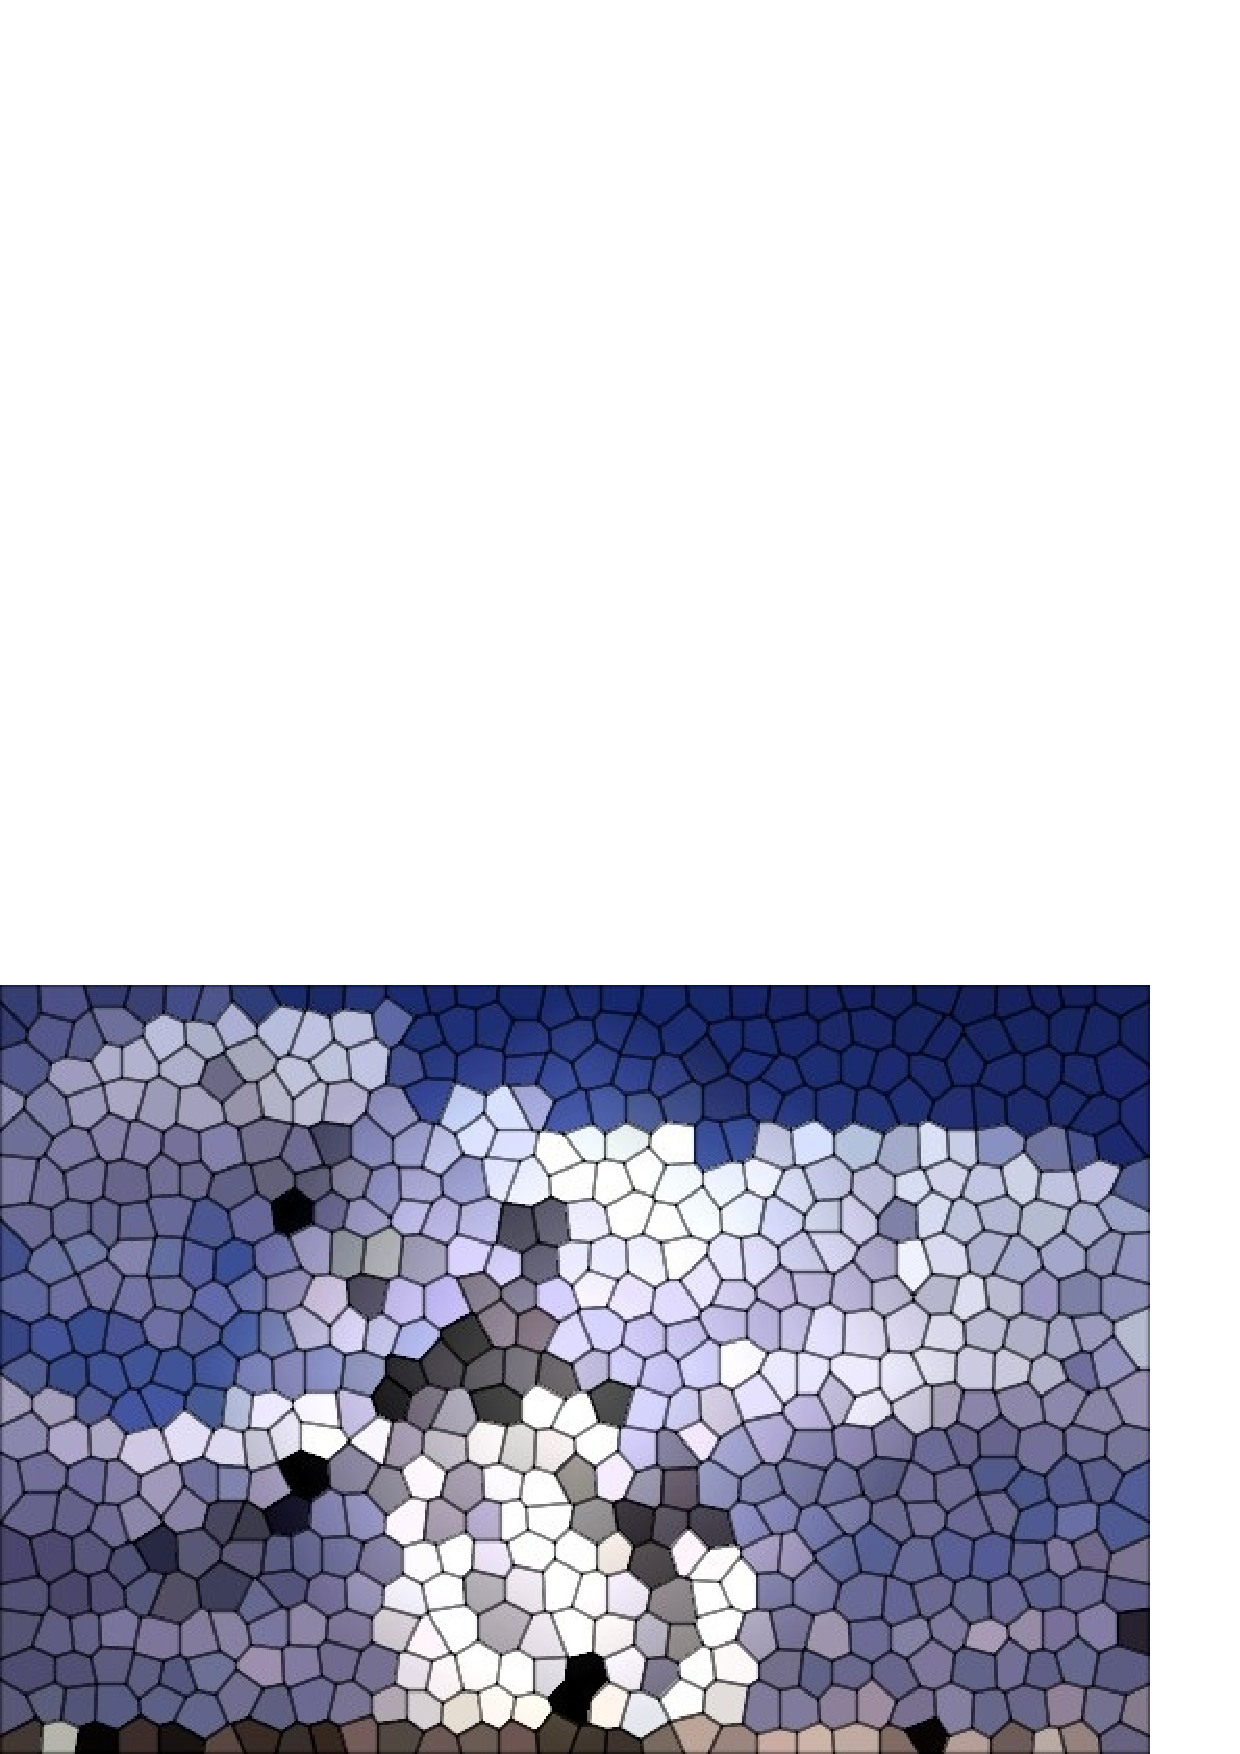
\includegraphics[scale=0.45]{img/introduction/sample_windmill1.pdf}

\emph{With a small sample size it's difficult to find the image content out!}
\end{center}
\end{frame}


%---------------------------------------------------------------------slide----
\begin{frame}
\frametitle{Sample size determination}
\framesubtitle{Large sample of pixels of a picture}
\begin{center}
What picture is it?

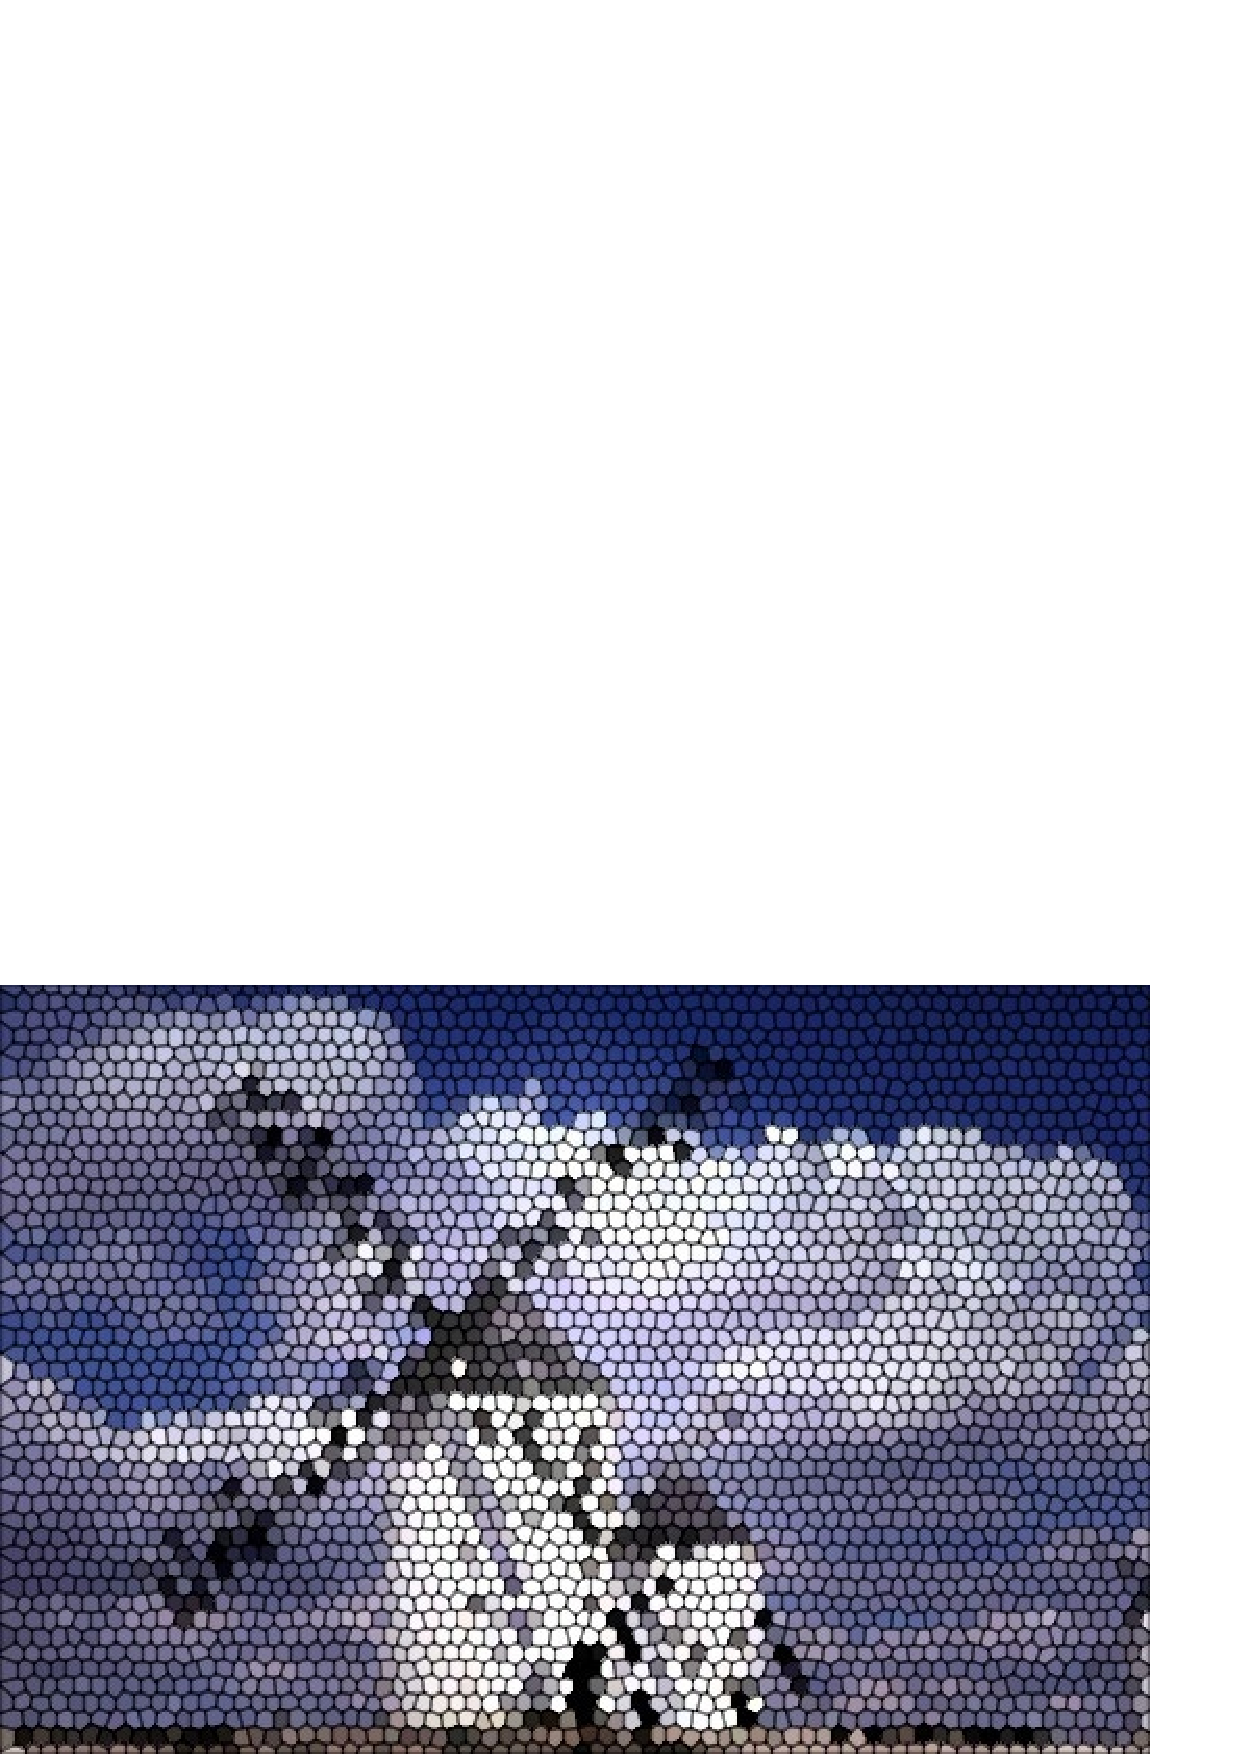
\includegraphics[scale=0.45]{img/introduction/sample_windmill2.pdf}

\emph{With a large sample is easier to find the image content out!}
\end{center}
\end{frame}


%---------------------------------------------------------------------slide----
\begin{frame}
\frametitle{Sample size determination}
\framesubtitle{Whole population of pixels of a picture}
\begin{center}
And here is the whole population.

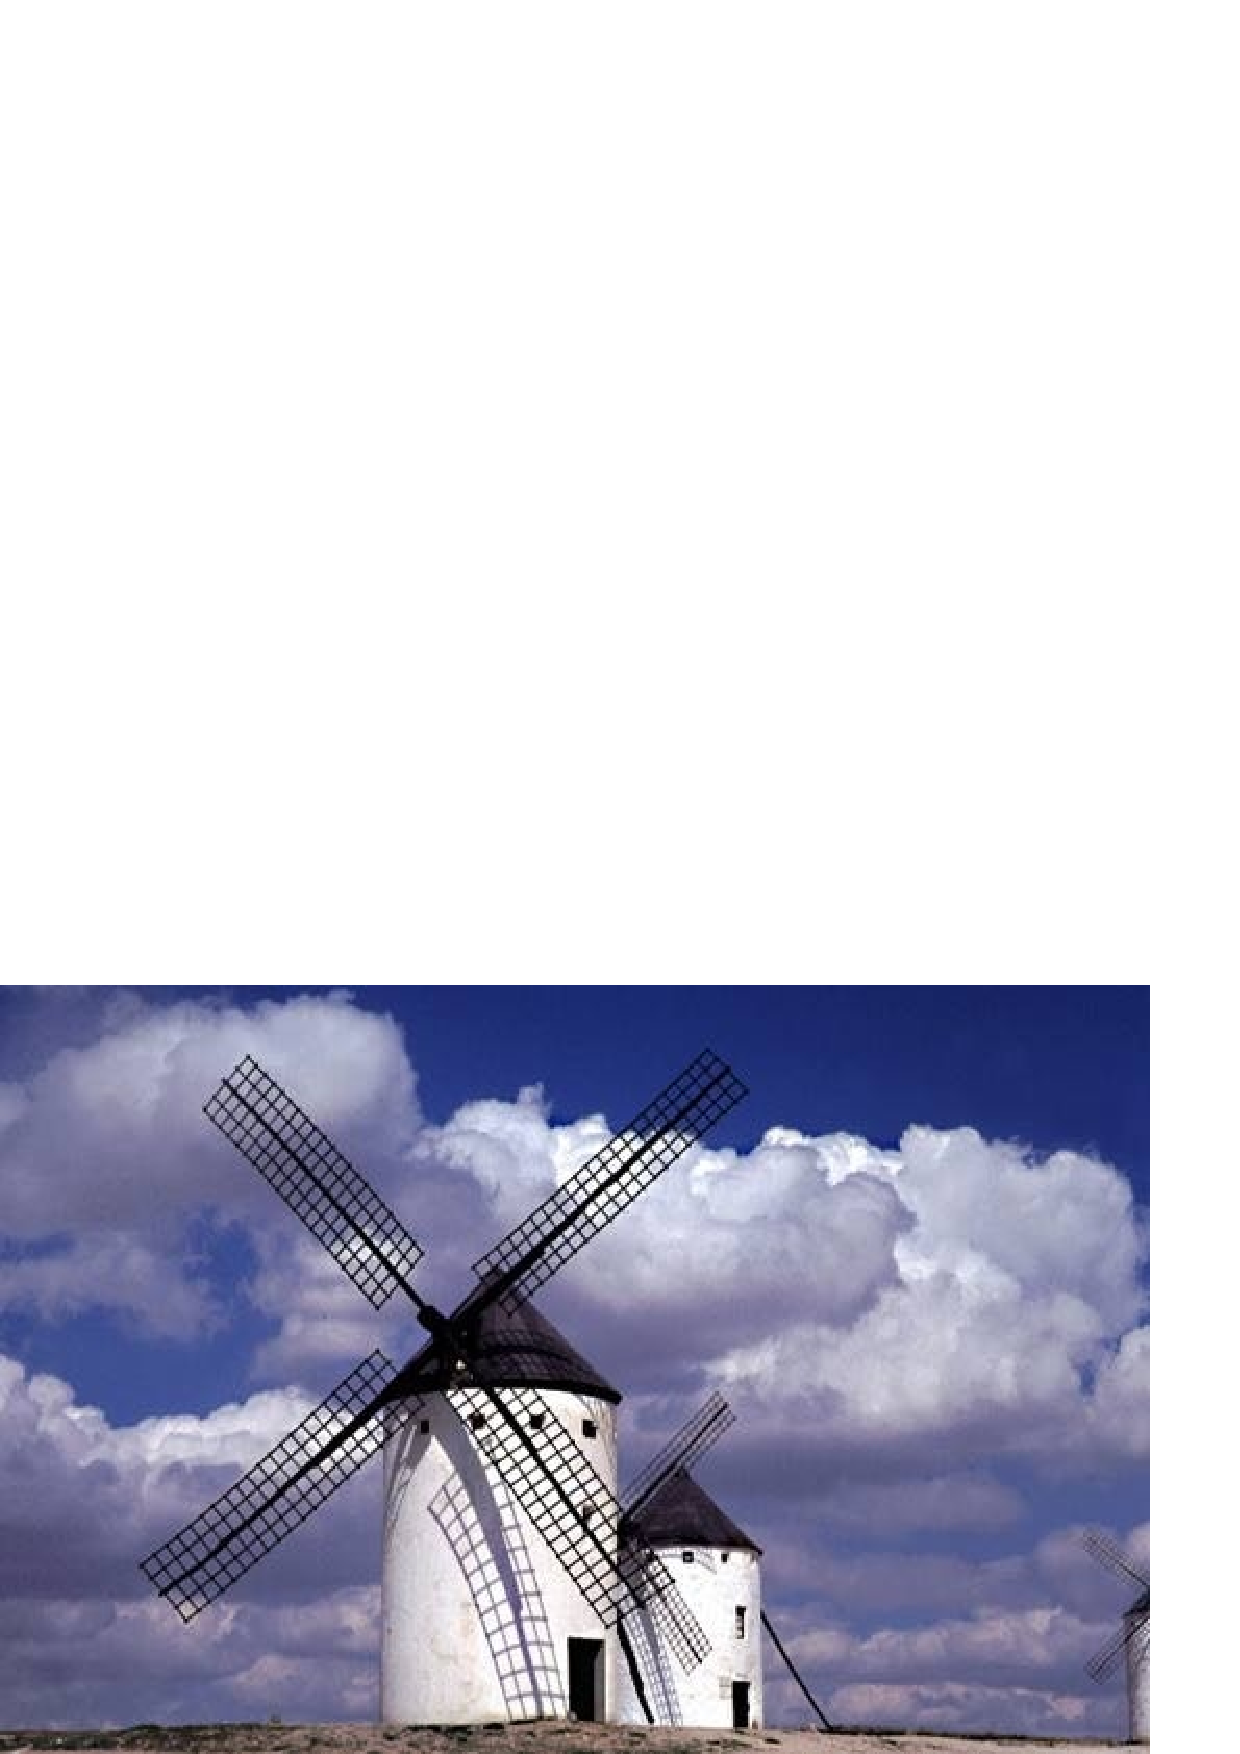
\includegraphics[scale=0.45]{img/introduction/sample_windmill3.pdf}

\emph{It's not required to know all the pixels of a picture to find their content out!}
\end{center}
\end{frame}


%---------------------------------------------------------------------slide----
\begin{frame}
\frametitle{Types of reasoning}

\begin{center}
\tikzsetnextfilename{introduction/types_reasoning}
% Autor: Alfredo Sánchez Alberca (email:asalber@ceu.es)
% Charts that shows the purpose of Statistics
\begin{tikzpicture}[every label/.style={text=color1}]
\tikzstyle{node} = [align=center, node distance=1cm]; 
\tikzstyle{arrow} = [-latex, color2, line width=10pt];

\node (population) [label=90:Population] at (0,5) {\includegraphics[height=1.5cm]{img/introduction/population.pdf}}; 
\node (sample) [label=-90:Sample] at (0,0) {\includegraphics[height=1.5cm]{img/introduction/sample.pdf}};
\draw[arrow] let \p1=(population.south), \p2=(sample.north) in (\x1-10,\y1) -- (\x2-10,\y2)
node[midway,rotate=-90,white] {Deduction};
\node[node] at (-2,2.5) {From general\\ to particular};
\pause
\draw[arrow] let \p1=(sample.north), \p2=(population.south) in (\x1+10,\y1) -- (\x2+10,\y2) 
node[midway,rotate=90,white] {Induction};
\node[node] at (2,2.5) {From particular\\ to general};
\end{tikzpicture} 
\end{center}
\end{frame}


% ---------------------------------------------------------------------slide----
\begin{frame}
\frametitle{Types of reasoning}
\begin{description}
\item [Deduction properties:] If the premises are true, it guarantees the certainty of the conclusions (that is, if
something is true in the population, it is also true in the sample). 
However, \alert{\emph{it does not provide new knowledge!}} 
\item [Induction properties:] It doesn't guarantee the certainty of the conclusions (if something is true in the
sample, it may not be true in the population, so be careful with the extrapolations!). 
But, \alert{\emph{¡it is the only way to generate new knowledge!}}
\end{description}

Statistics is fundamentally based on inductive reasoning, because it uses the information obtained from samples to
draw conclusions about populations.
\end{frame}


\subsection{Sampling}
%---------------------------------------------------------------------slide----
\begin{frame}
\frametitle{Sampling}
\begin{definition}[Sampling]
The process of selecting the elements included in a sample is known as \emph{sampling}.
\end{definition}
\begin{center}
\tikzsetnextfilename{introduction/sampling}
% Autor: Alfredo Sánchez Alberca (email:asalber@ceu.es)
% Charts that shows the purpose of Statistics
\begin{tikzpicture}[every label/.style={text=color1}]
\tikzstyle{node} = [align=center, node distance=1cm]; 
\tikzstyle{arrow} = [-latex, color2, line width=12pt];

\node (population) [label=-90:Population] at (0,0) {\includegraphics[height=2cm]{img/introduction/population.pdf}}; 
\node (sample) [label=-90:Sample] at (5,0) {\includegraphics[height=2cm]{img/introduction/sample.png}};
\draw[arrow] (population) -- (sample) node[midway,white] {Sampling\quad\phantom{0}};
\end{tikzpicture} 
\end{center}

To reflect reliable information about the whole population, the sample must be representative of the population.
That means that the sample should reproduce on a smaller scale the population variability.  

\begin{center}
\alert{\emph{Our goal is to get a representative sample!}}
\end{center}
\end{frame}


%---------------------------------------------------------------------slide----
\begin{frame}
\frametitle{Types of sampling}
There exists a lot of sampling methods but all of them can be grouped in two categories:
\begin{description}
\item[Random sampling] The sample individuals are selected randomly. 
All the population individuals have the same likelihood of being selected (equiprobability).  
\item[Non random sampling:] The sample individuals are not selected randomly. 
Some population individuals have a higher likelihood of being selected than others. 
\end{description}

Only random sampling methods avoid the selection bias and guarantee the representativeness of the sample, and therefore,
the validity of conclusions. 

Non random sampling methods are not suitable to make generalizations because doesn't guarantee the representativeness 
of the sample.
Nevertheless, usually are less expensive and can be used in exploratory studies. 
\end{frame}



%---------------------------------------------------------------------slide----
\begin{frame}
\frametitle{Simple random sampling}
The most popular random sampling method is the \emph{simple random sampling}, that has the following properties:
\begin{itemize}
\item All the population individuals have the same likelihood of being selected in the sample. 
\item The individual selection is performed with replacement, that is, each selected individual is returned to the
population before selecting the next one. 
This way the population doesn't change. 
\item Each individual selection is independent of the others. 
\end{itemize}

The only way of doing a random sampling is to assign a unique identity number to each population individual
(conducting a \emph{census}) and performing a random drawing.
\end{frame}


\subsection{Statistical variables}

%---------------------------------------------------------------------slide----
\begin{frame}
\frametitle{Statistical variables and data}
In every statistical study we are interested in some properties or characteristics of individuals. 
\begin{definition}[Statistical variable]
A \emph{statistical variable} is a property or characteristic measured in the population individuals. 

The \emph{data} is the actual values or outcomes recorded on a statistical variable. 
\end{definition}

\begin{center}
\tikzsetnextfilename{introduction/statistical_variables}
\includegraphics[scale=0.5]{img/introduction/statistical_variables.png}
\end{center}
\end{frame}


%---------------------------------------------------------------------slide----
\begin{frame}
\frametitle{Types of statistical variables}
According to the nature of their values and their scale, they can be:
\begin{itemize}
\item \structure{Qualitative variables:} They measure non-numeric qualities. 
They can be:
\begin{itemize}
\item \structure{Nominal:} There is no natural order between the categories.\\
Example: The eyes or hair colour. 
\item \structure{Ordinal:} There is a natural order between the categories. \\
Example: The education level.
\end{itemize}
\item \structure{Quantitative variables:} They measure numeric quantities. 
They can be:
\begin{itemize}
\item \structure{Discrete:} Their values are isolated numbers (usually integers).\\
Example: The number of children or cars in a family.
\item \structure{Continuous:} They can take any value in a real interval.\\
Example: The height, weight or age of a person. 
% They can be:
% \begin{itemize}
% \item \structure{Interval:} There is no absolute zero in the scale.\\
% Example: The temperature in degrees Celsius or Fahrenheit.
% \item \structure{Ratio:} There is an absolute zero in the scale.\\
% Example: The temperature in Kelvin, the height and weight.
%\end{itemize}
\end{itemize}
\end{itemize}
Qualitative and discrete variables are also called \emph{categorical variables} and their values \emph{categories}.
\end{frame}


%---------------------------------------------------------------------slide----
\begin{frame}
\frametitle{Types of statistical variables}
\begin{center}
\tikzsetnextfilename{introduction/variable_types}
% Author: Alfredo Sánchez Alberca (email:asalber@ceu.es)
% Types of statistical variables
\tikzset{every node/.style = {align=center, inner sep=2pt, text centered}}
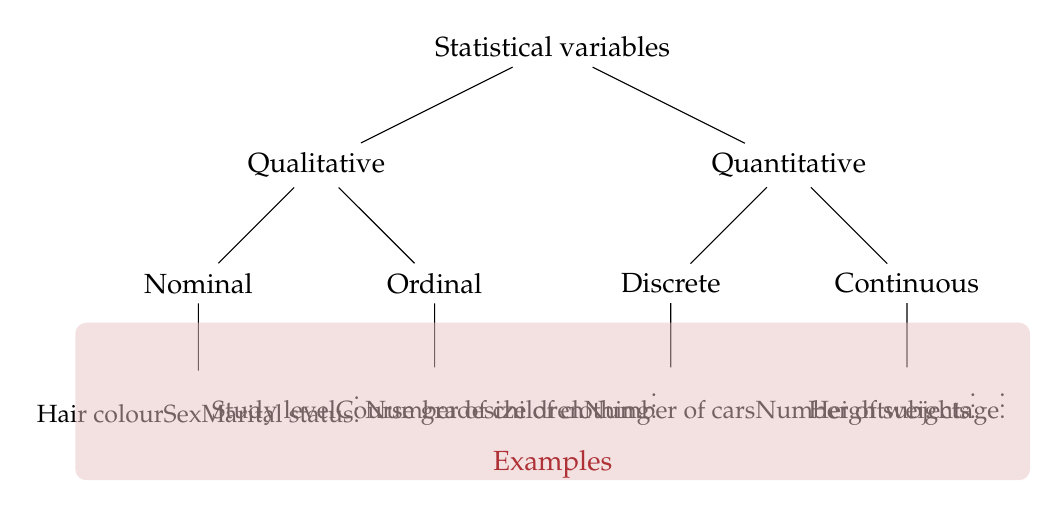
\begin{tikzpicture}[-, >=stealth', level distance = 1.5cm,
	level 1/.style={sibling distance = 6cm},
	level 2/.style={sibling distance = 3cm},
	level 3/.style={font=\small}
] 
\node {Statistical variables}
	child{node{Qualitative}
		child{node{Nominal}
			child{node{Hair colour\\ Sex\\ Marital status\\ $\vdots$}}
		}     
       	child{node{Ordinal}
			child{node{Study level\\ Course grade\\ size of clothing\\ $\vdots$}}
		}           
    }
	child{node{Quantitative}
		child{node{Discrete}
			child{node{Number of children\\ Number of cars\\ Number of subjects\\ $\vdots$}}
		}     
        child{node{Continuous}
			child{node{Height\\ weight\\ age\\ $\vdots$}}
%           	child{node{\parbox[top][1cm][t]{2cm}{Interval}}}
%            child{node{\parbox[top][1cm][t]{2cm}{Ratio}}}
        }               
    }
; 

\node [rectangle, minimum height=2cm, minimum width=\textwidth, fill=color1!30, rounded corners, opacity=0.5] at
(0,-4.5) {\phantom{0}}; 

\node [text=color1] at (0,-5.3) {Examples};
\end{tikzpicture}
\end{center}
\end{frame}



%---------------------------------------------------------------------slide----
\begin{frame}
\frametitle{Types of statistical variables}
\framesubtitle{Choosing the appropriate variable}
Sometimes a characteristic could be measured in variables of different types. 

\textbf{Example} Whether a person smokes or not could be measure in several ways: 
\begin{itemize}
\item Smokes: yes/no. (Nominal) 
\item Smoking level: No smoking/unusual/moderate/quite/heavy. (Ordinal)
\item Number of cigarettes per day: 0,1,2,\ldots (Discrete) 
\end{itemize} 

In those cases quantitative variables are preferable to qualitative, continuous variables are preferable to discrete
variables and ordinal variables are preferable to nominal, as they give more information. 

\begin{center}
\tikzsetnextfilename{introduction/variable_information}
\scalebox{1}{% Author: Alfredo Sánchez Alberca (email:asalber@ceu.es)
% Plot with the level of information of each variable type

\begin{tikzpicture}[scale=0.5]
\tikzstyle{node} = [align=center, text=color1];
\draw[stealth-stealth, thin, color1!90, line width=12pt] (-0.5,4) -- (18.5,4);
\node at (1.5,4) {\color{white}-- Info};
\node at (16.5,4) {\color{white} + Info};
\node[node] at (1,2.5) {Nominal};
\node[node] at (5,2.5) {Ordinal};
\node[node] at (9,2.5) {Discrete};
\node[node] at (13,2.5) {Interval};
\node[node] at (17,2.5) {Ratio};
\end{tikzpicture}} 
\end{center}
\end{frame}


%---------------------------------------------------------------------slide----
\begin{frame}
\frametitle{Types of statistical variables}
According to their role in the study:
\begin{itemize}
\item \structure{Independent variables:} Variables that no depends on other variables in the study. 
Usually they are manipulate in an experiment in order to observe their effect on a dependent variable.
They are also known as \emph{predictor variables}. 
\item \structure{Dependent variables:} Variables that depends on other variables in the study.
They are not manipulated in an experiment and are also known as \emph{outcome variables}. 
\end{itemize}

\textbf{Example} In a study on the performance of students in a course, the intelligence of students and the daily
study time are independent variables, while the course grade is a dependent variable. 
\end{frame}


%---------------------------------------------------------------------slide----
\begin{frame}
\frametitle{Types of statistical studies}
According to their role in the study:
\begin{itemize}
\item \structure{Experimental:} When the independent variables are manipulated in order to see the effect that that
change have on the dependent variables.\\
\textbf{Example} In a study on the performance of students in a test, the teacher manipulates the study time and create
two or more groups asking students in each group to study a different number of hours. 
\item \structure{Non-experimental:} When the independent variables are not manipulated. That not means that it is
impossible to do so, but it will either be impractical or unethical to do so.\\
\textbf{Example} In a study a researcher could be interested in the effect of smoking over the lung
cancer. 
However, whilst possible, it would be unethical to ask individuals to smoke in order to study what effect this had on
their lungs. In this case, the researcher could study two groups of people, one with lung cancer and other
without, an observe in each group how many persons smoke or not. 
\end{itemize}

Experimental studies allow to identify a cause and effect between variables while non-experimental studies
only allow to identify association or relationship between variables. 
\end{frame}


%---------------------------------------------------------------------slide----
\begin{frame}
\frametitle{The data table}
The variables of a study will be measured in each individual of the sample. 
This will give a data set that usually is arranged in a tabular form known as \structure{\textbf{data table}}.

In this table each column contains the information of a variable and each row contains the information of an individual. 

\textbf{Example}
\begin{center}
\begin{tabular}{|l|c|c|c|c|}
\hline
Name & Age & Gender & Weight(Kg) & Height (cm)\\
\hline
José Luis Martínez & 18 & M &  85 & 179 \\
Rosa Díaz & 32 & F & 65 & 173 \\
Javier García & 24 & M & 71 & 181 \\
Carmen López & 35 & F &  65 & 170 \\
Marisa López  & 46 & F &  51 & 158 \\
Antonio Ruiz & 68 & M & 66 & 174 \\
\hline
\end{tabular}
\end{center}
\end{frame}


\subsection{Phases of a statistical study}

%---------------------------------------------------------------------slide----
\begin{frame}
\frametitle{Phases of a statistical study}
Usually a statistical study goes through the following phases:  
\begin{enumerate}
\item The study begins with a previous design in which are set the study goals, the population, the variables to
measure and the required sample size.
\item Next, the sample is selected from the population and the variables are measured in the individuals of the sample
(getting the data table).
This is accomplished by \emph{sampling}.  
\item The next step consists in describing and summarizing the information of the sample. 
This is the job of \emph{Descriptive statistics}. 
\item Then, the information obtained is projected on a mathematical model that intend to explain what happens in
population, and the model is validated. 
This is accomplished by \emph{Inferential statistics}.
\item Finally, the validated model is used to perform predictions and to draw conclusions on the population.
\end{enumerate}
\end{frame}


%---------------------------------------------------------------------slide----
\begin{frame}
\frametitle{The statistical cycle}
\begin{center}
\tikzsetnextfilename{introduction/statistical_cycle}
% Author: Alfredo Sánchez Alberca (email:asalber@ceu.es)
% Plot with the phases of the statistical cycle
\begin{tikzpicture}[every label/.style={text=color1}]
\tikzstyle{arrow} = [-latex, color1, line width=12pt];
\tikzstyle{node} = [align=center, inner sep=10pt];
\node[node, label=-90:Population] (population) at (1,1)
{\includegraphics[height=1.5cm]{img/introduction/population}}; 
\pause
\node[node,label=90:Sample] (sample) at
(1,6){\includegraphics[height=1.5cm]{img/introduction/sample.png}}; 
\node at (1,3.4) [fill=color1,single arrow,shape border rotate=90,text=white, minimum width=1.2cm, minimum
height=3cm]{
\rotatebox{90}{Sampling}\phantom{}};
\pause
\node[node,label=90:Summary measures] (statistics) at (8,6) {\Large $\bar x$ \quad $s^2$\\\Large \quad $p$ \quad
$g_1$}; 
\node at (4.5,6) [fill=color1,single arrow,shape border rotate=0,text=white, minimum width=1.2cm, minimum
height=3cm]{
Descriptive Statistics\phantom{}};
\pause
\node[node,label=-90:Model] (model) at (8,1) {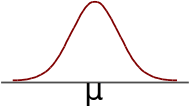
\includegraphics[scale=0.5]{img/introduction/normal}};
\node at (8,3.6) [fill=color1,single arrow,shape border rotate=270,text=white, minimum width=1.2cm, minimum
height=3cm]{
\rotatebox{90}{Inferential Stat.}\phantom{}};
\pause
\node at (4.5,1) [fill=color1,single arrow,shape border rotate=180,text=white, minimum width=1.2cm, minimum
height=3cm]{ Prediction\phantom{}};
\end{tikzpicture}
\end{center}
\end{frame}


\section{Estadística Descriptiva}

\mode<presentation>{
%---------------------------------------------------------------------slide----
\begin{frame}
\frametitle{Estadística Descriptiva}
\tableofcontents[sectionstyle=show/hide,hideothersubsections]
\end{frame}
}


%---------------------------------------------------------------------slide----
\begin{frame}
\frametitle{Estadística descriptiva}
La estadística descriptiva es la parte de la estadística encargada de representar, analizar y resumir la información contenida en la muestra.

Tras el proceso de muestreo, es la siguiente etapa de todo estudio estadístico y suele consistir en:
\begin{enumerate}
\item Clasificar, agrupar y ordenar los datos de la muestra.
\item Representar dichos datos gráficamente y en forma de tablas.
\item Calcular medidas que resuman la información que contiene la muestra (\emph{estadísticos muestrales}).
\end{enumerate} 

Su poder inferencial es mínimo, por lo que nunca deben sacarse conclusiones sobre la población a partir de las medidas resumen que aporta la estadística descriptiva.
\note{Como se vió en el tema introductorio, la estadística trata de conocer las poblaciones a partir del estudio de
muestras. Una vez obtenida la muestra de la población, el siguiente paso en cualquier estudio estadístico es el
análisis descriptivo de la muestra y este es el objeto la estadística descriptiva, que es la parte de la estadística
encargada de representar, analizar y resumir la información contenida en la muestra. El objetivo es exprimir bien la
muestra para sacarle toda la información posible y sintetizar dicha información para hacerla comprensible.

Las tareas que realiza la estadística descriptiva suelen ser:
\begin{enumerate}
\item Clasificar, agrupar y ordenar los datos de la muestra.
\item Representar dichos datos gráficamente y en forma de tablas.
\item Calcular medidas que resuman la información que contiene la muestra (\emph{estadísticos muestrales}).
\end{enumerate} 

Aunque una buena descripción de la muestra facilita el posterior conocimiento de la población, nunca deben sacarse
conclusiones sobre la población a partir de las medidas resumen que aporta la estadística descriptiva, ya que de esto
se encarga la estadística inferencial que se vera más adelante en este curso.}
\end{frame}


%---------------------------------------------------------------------slide----
\begin{frame}
\frametitle{Clasificación de la muestra}
El estudio de una variable estadística comienza por medir la variable en los individuos de la muestra y clasificar los valores obtenidos.

Existen dos formas de clasificar estos valores:
\begin{description}
\item[Sin agrupar:] Ordenar todos los valores obtenidos en la muestra de menor a mayor. Se utiliza con atributos y variables discretas con pocos valores diferentes.
\item[Agrupados:] Agrupar los valores en clases (intervalos) y ordenar dichas clases de menor a mayor. Se utiliza con variables discretas con muchos valores diferentes, y con variables continuas.
\end{description}
\note{La matriz de datos contiene toda la información de la muestra pero resulta difícil de interpretar, por lo que para
sintetizar y resumir esa información se realizan varias tareas que empiezan por la clasificación de los valores. 

Esta clasificación consiste en ordenar los valores de menor a mayor, cuando existe un orden entre dichos valores, o
simplemente en reunir los valores iguales cuando no hay un orden entre ellos.

En las variables cuantitativas, cuando el número de valores distintos es muy grande, estos suelen agruparse en
intervalos.}
\end{frame}


\subsection{Distribución de frecuencias}

%---------------------------------------------------------------------slide----
\begin{frame}
\frametitle{Clasificación de la muestra}
\begin{center}
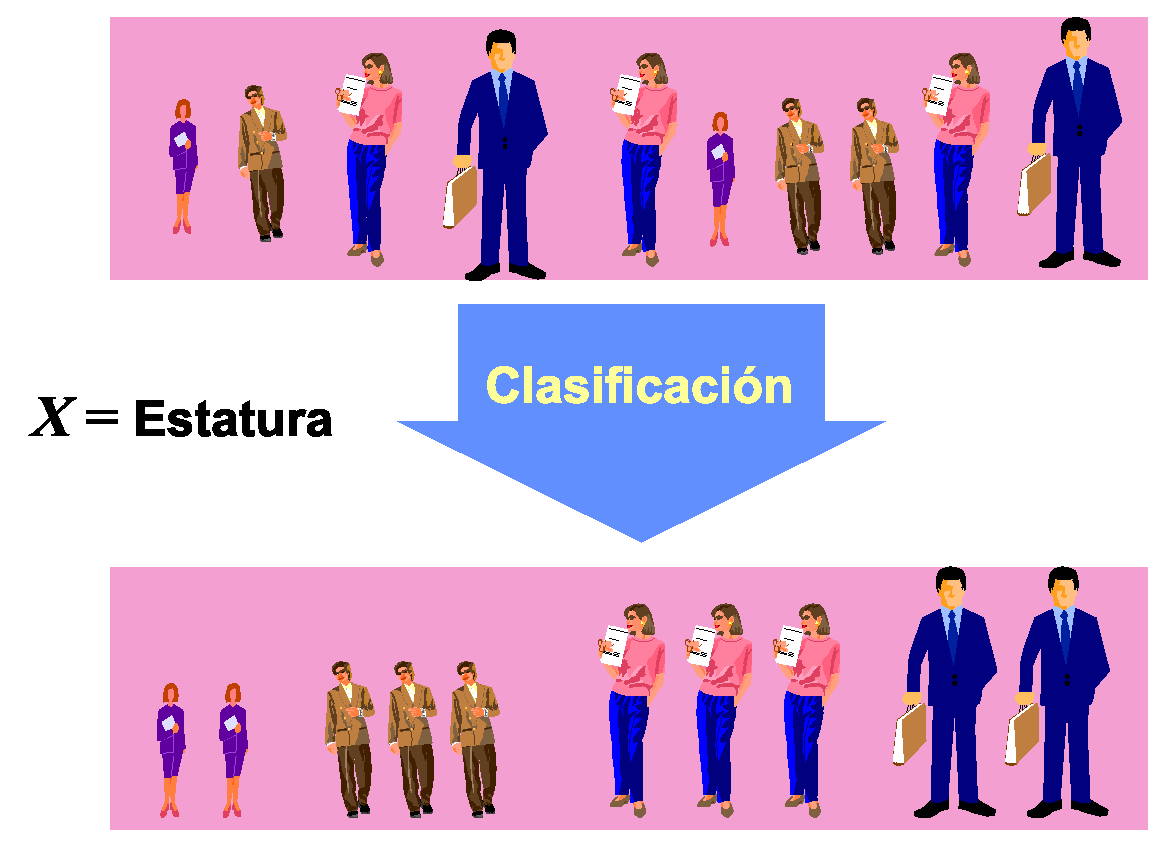
\includegraphics[scale=0.5]{img/descriptiva/clasificacion_muestra}
\end{center}
\note{En este ejemplo tenemos una muestra de 10 individuos en los que se ha medido su estatura. Como se trata de una
variable cuantitativa, la clasificación consiste, primero en ordenar las estaturas de menor a mayor.}
\end{frame}


%---------------------------------------------------------------------slide----
\begin{frame}
\frametitle{Recuento de frecuencias}
\begin{center}
\includegraphics[scale=0.5]{img/descriptiva/recuento_frecuencias}
\end{center}
\note{Y a continuación, si hay valores repetidos, contar la frecuencia de repetición de cada estatura o cuántas
estaturas caen en cada uno de los intervalos que hayamos definido en caso de agrupar los datos. Por ejemplo, la primera
estatura se repite dos veces y por tanto tiene frecuencia 2, la segunda estatura se repite tres veces y tiene frecuencia 3 y así sucesivamente. 
}
\end{frame}


%---------------------------------------------------------------------slide----
\begin{frame}
\frametitle{Frecuencias muestrales}
\begin{definicion}[Frecuencias muestrales]
Dada una muestra de tamaño $n$ de una variable $X$, para cada valor de la variable $x_i$ observado en la muestra, se define
\begin{itemize}
\item \structure{Frecuencia absoluta $n_i$}: Es el número de individuos de la
muestra que presentan el valor $x_i$.
\item \structure{Frecuencia relativa $f_i$}: Es la proporción de individuos de
la muestra que presentan el valor $x_i$. 
\[
f_i = \frac{n_i}{n}
\]
\item \structure{Frecuencia absoluta acumulada $N_i$}: Es el número de
individuos de la muestra que presentan un valor menor o igual que $x_i$.
\[
N_i = n_1 + \cdots + n_i
\]
\item \structure{Frecuencia relativa acumulada $F_i$}: Es la proporción de
individuos de la muestra que presentan un valor menor o igual que $x_i$.
\[
F_i = \frac{N_i}{n}
\]
\end{itemize}
\end{definicion}
\note{Existen distintos tipos de frecuenicas que pueden calcularse. 
Dada una muestra de tamaño $n$ de una variable $X$, para cada valor de la variable $x_i$ observado en la muestra, se define
\begin{itemize}
\item La frecuencia absoluta, que se representa como $n_i$, es el número de individuos de la
muestra que presentan el valor $x_i$, es decir el número de veces que se repite dicho valor.
\item La frecuencia relativa, que se denota $f_i$, es la proporción de individuos de
la muestra que presentan el valor $x_i$. La frecuencia relativa se calcula dividiendo la frecuencia absoluta entre el
tamaño de la muestra.
\[
f_i = \frac{n_i}{n}
\]
Cuando se multiplica por 100 se convierte en un porcentaje.
\item La frecuencia absoluta acumulada, que se escribe $N_i$, es el número de
individuos de la muestra que presentan un valor menor o igual que $x_i$. Se calcula acumulando las frecuencias
absolutas de los valores menores o iguales a $x_i$ y de ahí su nombre.
\[
N_i = n_1 + \cdots + n_i
\]
\item La frecuencia relativa acumulada, que se escribre $F_i$, es la proporción de
individuos de la muestra que presentan un valor menor o igual que $x_i$. Puede calcularse acumulando las frecuencias
relativas de los valores menores o iguales que $x_i$ o bien dividiendo la frecuencia absoluta cumulada de $x_i$ entre
el tamaño de la muestra.
\[
F_i = \frac{N_i}{n}
\]
Al igual que la frecuencia relativa, si se multiplica por 100 se convierte en el porcentaje acumulado.
\end{itemize}
 }
\end{frame}


%---------------------------------------------------------------------slide----
\begin{frame}
\frametitle{Tabla de frecuencias}
Al conjunto de valores observados en la muestra junto a sus respectivas frecuencias se le denomina \structure{\textbf{distribución muestral de frecuencias}} y suele representarse mediante una \structure{\textbf{tabla de frecuencias}}.
\begin{center}
\begin{tabular}{|>{\centering}p{1.8cm}|>{\centering}p{1.8cm}|>{\centering}p{1.8cm}|>{\centering}p{1.8cm}|p{1.8cm}<{\centering}|}
\hline
\structure{Valores de $X$} & \structure{Frecuencia Absoluta} & \structure{Frecuencia Relativa} & \structure{Frecuencia Absoluta Acumulada} & \structure{Frecuencia Relativa Acumulada} \\
\hline
$x_1$ & $n_1$ & $f_1$ & $N_1$ & $F_1$\\
$\vdots$ & $\vdots$ & $\vdots$ & $\vdots$ & $\vdots$\\
$x_i$ & $n_i$ & $f_i$ & $N_i$ & $F_i$\\
$\vdots$ & $\vdots$ & $\vdots$ & $\vdots$ & $\vdots$\\
$x_k$ & $n_k$ & $f_k$ & $N_k$ & $F_k$\\
\hline
\end{tabular}
\end{center}
\note{Normalmente las frecuencias muestrales suelen organizarse en forma de tabla en la que cada fila corresponde a un
valor de la variable o un intervalo de valores, que se ordenan, siempre que sea posible, de menor a mayor, y cada
columna corresponde a una frecuencia.

En esta tabla siempre se debe cumplir que la suma de las frecuencias absolutas es igual al tamaño de la muestra, la
suma de las frecuencias relativas vale 1, la última frecuencia absoluta acumulada es el tamaño de la muestra y la
última frecuencia relativa acumulada es 1. De no ser así, habríamos cometido algún error en el cálculo de las
frecuencias.}
\end{frame}


%---------------------------------------------------------------------slide----
\begin{frame}
\frametitle{Tabla de frecuencias}
\framesubtitle{Ejemplo de datos sin agrupar}
En una encuesta a 25 matrimonios sobre el número de hijos que tenían se obtuvieron los siguientes datos:
\begin{center}
1, 2, 4, 2, 2, 2, 3, 2, 1, 1, 0, 2, 2, \\
 0, 2, 2, 1, 2, 2, 3, 1, 2, 2, 1, 2
\end{center}
La tabla de frecuencias asociada a esta muestra es
\[
\setlength\arraycolsep{3mm}
\setlength\arrayrulewidth{0.5pt}
\begin{array}{rrrrr}
\hline
x_i & n_i & f_i & N_i & F_i\\
\hline
0 & 2 & 0.08 & 2 & 0.08\\
1 & 6 & 0.24 & 8 & 0.32\\
2 & 14 & 0.56 & 22 & 0.88\\
3 & 2  & 0.08 & 24 & 0.96\\
4 & 1 & 0.04 & 25 & 1 \\ 
\hline 
\sum & 25 & 1 \\
\hline
\end{array}
\]
\note{En este ejemplo se han tomado 25 matrimonios en los que se ha medido el número de hijos que tenían. Se trata de
una variable cuantitativa discreta puesto que sólo puede tomar valores enteros positivos y además en la muestra sólo
aparece 5 valores disntintos que son 0, 1, 2, 3 y 4 hijos, por lo que no es necesario agrupar los datos en intervalos.

Para construir la tabla de frecuencias se comienza por el recuento de las frecuencias absolutas. Como puede observarse
en la muestra, hay dos matrimonios que tienen 0 hijos, y por tanto, la frecuencia absoluta del 0 es 2, el 1
aparece 6 veces, el 2, 3 veces, el 3, 2 veces y finalmente el 4 sólo aparece una vez. Observese cómo la suma de las
frecuencias absolutas da 25 que es el tamaño muestral.

A continuación se calculan las frecuencias relativas, simplemente dividiendo cada frecuencia absoluta por el tamaño de
la muestra que es 25. Por ejemplo, la frecuencia relativa del 0 es 2 entre 25 que es 0.08, y es la proporción de
matrimonios en la muestra que tienen 0 hijos.  Si se multiplica por 100 da un 8\%, es decir, el 8\% de los matrimonios
tienen 0 hijos. Obsérvese cómo la suma de las frecuencias relativas vale 1. 

Después se calculan las frecuencias absolutas acumuladas. Así, por ejemplo, la frecuencia absoluta acumulada del 0 es
el número de matrimonios que tienen 0 o menos hijos, y al ser el 0 el menor de los valores de la muestra, coincide con
la su frecuencia absoluta, que vale 2. La frecuencia absoluta acumulada del 1 es el número de matrimonios que tienen 1
o menos hijos, de manera que habría que acumula la frecuencia absoluta del 1 y del 0, es decir, 2 mas 6, que da un
total de 8, y así sucesivamente. En general para calcular cada frecuencia absoluta acumulada se puede tomar la
frecuencia absoluta acumulada anterior y sumarle la frecuencia absoluta del valor. 8+14=22, 22+2=24 y 24+1=25.
Obsérvese cómo la última frecuencia absoluta acumulada vale 25 que es el tamaño de la muestra.

Finalmente, se calculan las frecuencias relativas acumuladas, que pueden calcularse, bien acumulando las frecuencias
relativas del mismo modo que se acumulaban las absolutas, o bien dividiendo las frecuencias absolutas acumuladas por el
tamaño de la muestra. Así, por ejemplo, la frecuencia relativa acumulada del 0 es 2 entre 25, que vale 0.08 y coincide
con su frecuencia relativa. La frecuencia relativa acumulada del 1 es 8 entre 25 que vale 0.32 y es la proporción de
matrimonios en la muestra con 1 o menos hijos. Si se multiplica por 100 tenemos que hay un 32\% de matrimonios con 1 o
menos hijos. Y del mismo modo se calculan el resto de frecuencias relativas acumuladas, hasta llegar a la última que
siempre vale 1.
}
\end{frame}


%---------------------------------------------------------------------slide----
\begin{frame}
\frametitle{Tabla de frecuencias}
\framesubtitle{Ejemplo de datos agrupados}
Se ha medido la estatura (en cm) de 30 universitarios obteniendo:
\begin{center}
179, 173, 181, 170, 158, 174, 172, 166, 194, 185,\\
162, 187, 198, 177, 178, 165, 154, 188, 166, 171,\\
175, 182, 167, 169, 172, 186, 172, 176, 168, 187.
\end{center}
La tabla de frecuencias asociada a esta muestra es
\[
\setlength\arraycolsep{3mm}
\setlength\arrayrulewidth{0.5pt}
\begin{array}{rrrrr}
\hline
\multicolumn{1}{c}{x_i} & \multicolumn{1}{c}{n_i} & \multicolumn{1}{c}{f_i} & \multicolumn{1}{c}{N_i} & \multicolumn{1}{c}{F_i}\\
\hline
(150,160] & 2 & 0.07 & 2 & 0.07\\
(160,170] & 8 & 0.27 & 10 & 0.34\\
(170,180] & 11 & 0.36 & 21 & 0.70\\
(180,190] & 7  & 0.23 & 28 & 0.93\\
(190,200] & 2 & 0.07 & 30 & 1 \\ 
\hline 
\sum & 30 & 1 \\
\hline
\end{array}
\]
\note{En este otro ejemplo, se han medido las estaturas de 30 universitarios. Ahora se trata de una variable
cuantitativa continua, y como siempre ocurre con este tipo de variables, el número de valores disntintos que aparece en
la muestra suele ser demasiado grande, por lo que se tiene a agruparlos en intervalos.

En este caso se ha optado por construir 5 intervalos de amplitud 10 cm, empezando en 150 cm y terminando en 200 cm. 

El cálculo de frecuencias absolutas es similar al caso anterior, salvo que ahora no se cuenta el número de estaturas
que se repiten, sino el número de estaturas que caen en cada intervalo. Por ejemplo, la frecuencia
absoluta del intervalo $(150,160]$ es 2 ya que en la muestra hay dos personas, una que mide 158 y otra que mide 154, que caerían en este intervalo.
Una vez calculadas las frecuencias abolutas, el cálculo del resto de frecuencias es idéntico al caso de datos no
agrupados.}
\end{frame}


%---------------------------------------------------------------------slide----
\begin{frame}
\frametitle{Construcción de clases}
Cada intervalo de agrupación de datos se denomina \structure{\textbf{clase}} y el centro del intervalo se llama \structure{\textbf{marca de clase}}.

A la hora de agrupar los datos en clases hay que tener en cuenta lo siguiente:
\begin{itemize}
\item El número de intervalos no debe ser muy grande ni muy pequeño. Una regla
orientativa es tomar un número de intervalos próximo a la raíz cuadrada del
tamaño muestral $\sqrt{n}$. 
\item Los intervalos no deben solaparse y deben cubrir todo el rango de valores.
Es indiferente si se abren por la izquierda y se cierran por la derecha o al revés.
\item El valor más pequeño debe caer dentro del primer intervalo y el más grande dentro del último.
\end{itemize}
\note{Cada intervalo de agrupación de datos se denomina clase y el centro del intervalo se llama
marca de clase. 
Cuando se decide agrupar los datos en clases, hay que tener en cuenta lo siguiente:
\begin{itemize}
\item En primer lugar, el número de intervalos no debe ser muy grande ni muy pequeño. Si hay muchos intervalos, la
tabla será enorme y no sintetizará bien la información de la muestra, mientras que si tomamos muy pocos intervalos, su
amplitud será muy grande y se perderá gran parte de la información que contiene la muestra, ya que cuando un individuo
se cuenta dentro de un intervalo, pierde su valor particular y pasa a ser representado por la marca de clase. Una regla
orientativa es tomar un número de intervalos próximo a la raíz cuadrada del tamaño muestral $\sqrt{n}$.
\item En segundo lugar, los intervalos no deben solaparse, ya que de lo contrario se correría el riesgo de que algún
individuo cayese en dos intervalos distintos, por eso se suelen construir intervalos abiertos por la izquierda y
cerrados por la derecha o al revés, pero siempre siguiendo el mismo criterio. Y también deben cubrir todo el rango de
valores, ya que de lo contrario se correría el riesgo de que algún individuo no caería en ningún intervalo y quedaría
sin contarse.
\item Por último, el valor más pequeño debe caer dentro del primer intervalo y el más grande dentro del último.
\end{itemize}}
\end{frame}


%---------------------------------------------------------------------slide----
\begin{frame}
\frametitle{Tabla de frecuencias}
\framesubtitle{Ejemplo con un atributo}
Los grupos sanguíneos de una muestra de 30 personas son:
\begin{center}
A, B, B, A, AB, 0, 0, A, B, B, A, A, A, A, AB,\\
A, A, A, B, 0, B, B, B, A, A, A, 0, A, AB, 0. 
\end{center}
La tabla de frecuencias asociada a esta muestra es
\[
\setlength\arraycolsep{3mm}
\setlength\arrayrulewidth{0.5pt}
\begin{array}{crr}
\hline
\multicolumn{1}{c}{x_i} & \multicolumn{1}{c}{n_i} & \multicolumn{1}{c}{f_i} \\
\hline
\mbox{0} & 5 & 0.16 \\
\mbox{A} & 14 & 0.47 \\
\mbox{B} & 8 & 0.27 \\
\mbox{AB} & 3 & 0.10 \\
\hline 
\sum & 30 & 1 \\
\hline
\end{array}
\]
\begin{center}
\emph{¿Por qué en este caso no se construyen las columnas de frecuencias acumuladas?}
\end{center}
\note{En este otro ejemplo, se ha medido el grupo sanguíneo de un grupo de 30 personas. Ahora se trata de un atributo
nominal, de manera que como no hay orden entre sus valores, puden ordenarse de cualquier manera en la tabla de
frecuencias, pero el cálculo de frecuencias se realiza como en casos anteriores, con la particularidad de que en este
caso no tiene sentido calcular las frecuencias acumuladas. ¿Te imaginas por qué?}
\end{frame}


\subsection{Representaciones gráficas}

%---------------------------------------------------------------------slide----
\begin{frame}
\frametitle{Representaciones gráficas}
También es habitual representar la distribución muestral de frecuencias de forma gráfica.
Dependiendo del tipo de variable y de si se han agrupado o no los datos, se utilizan distintos tipos de gráficos:
\begin{itemize}
\item \structure{Diagrama de barras}: Consiste en un diagrama sobre el plano
cartesiano en el que en el eje $X$ se representan los valores de la variable y en el eje $Y$ las frecuencias. Sobre cada valor de la variable se levanta una barra de altura la correspondiente frecuencia. 
Se utiliza con variables discretas no agrupadas.
\item \structure{Histograma}: Es similar a un diagrama de barras pero
representando en el eje $X$ las clases en que se agrupan los valores de la variable y levantando las barras sobre todo el intervalo de manera que las barras están pegadas unas a otras. 
Se utiliza con variables discretas agrupadas y con variables continuas. 
\item \structure{Diagrama de sectores}: Consiste en un círculo dividido
en sectores de área proporcional a la frecuencia de cada valor de la variable.
Se utiliza sobre todo con atributos.  
\end{itemize}
En cada uno de los diagramas pueden representarse los distintos tipos de frecuencias, siempre que estas existan.
\note{Habitualmente las frecuencias también suelen representarse de manera gráfica. Dependiendo del tipo de variable y
de si se han agrupado o no los datos, se utilizan distintos tipos de gráficos, entre los que cabe destacar los
diagramas de barras, los histogramas y los diagramas de sectores. Veamos un ejemplo de cada uno de ellos.}
\end{frame}


%---------------------------------------------------------------------slide----
\begin{frame}
\frametitle{Diagrama de barras de frecuencias absolutas}
\framesubtitle{Datos sin agrupar}
\begin{center}
\scalebox{0.75}{%% Input file name: diagrama_barras_frecuencia_absoluta.fig
%% FIG version: 3.2
%% Orientation: Landscape
%% Justification: Flush Left
%% Units: Inches
%% Paper size: A4
%% Magnification: 100.0
%% Resolution: 1200ppi

\begin{pspicture}(6.70cm,3.48cm)(16.66cm,13.45cm)
\psset{unit=0.8cm}
%%
%% Depth: 2147483647
%%
\newgray{mycolor0}{0.74}\definecolor{mycolor0}{gray}{0.74}
\newrgbcolor{mycolor1}{1.00 0.50 0.31}\definecolor{mycolor1}{rgb}{1.00,0.50,0.31}
%%
%% Depth: 100
%%
\psset{linestyle=solid,linewidth=0.03175,linecolor=black,fillstyle=solid,fillcolor=mycolor0}
\pspolygon(10.92,6.47)(10.92,6.47)(12.47,6.47)(12.47,6.47)(10.92,6.47)
\psset{fillstyle=none}
\psline(10.23,6.47)(10.23,15.28)
\psline(10.23,6.47)(10.02,6.47)
\psline(10.23,7.73)(10.02,7.73)
\psline(10.23,8.99)(10.02,8.99)
\psline(10.23,10.25)(10.02,10.25)
\psline(10.23,11.50)(10.02,11.50)
\psline(10.23,12.76)(10.02,12.76)
\psline(10.23,14.02)(10.02,14.02)
\psline(10.23,15.28)(10.02,15.28)
\rput{90}(9.73,6.47){0}
\rput{90}(9.73,7.73){2}
\rput{90}(9.73,8.99){4}
\rput{90}(9.73,10.25){6}
\rput{90}(9.73,11.50){8}
\rput{90}(9.73,12.76){10}
\rput{90}(9.73,14.02){12}
\rput{90}(9.73,15.28){14}
\psset{linestyle=dotted,linecolor=mycolor0}
\psline(10.23,6.47)(20.31,6.47)
\psline(10.23,7.73)(20.31,7.73)
\psline(10.23,8.99)(20.31,8.99)
\psline(10.23,10.25)(20.31,10.25)
\psline(10.23,11.50)(20.31,11.50)
\psline(10.23,12.76)(20.31,12.76)
\psline(10.23,14.02)(20.31,14.02)
\psset{linestyle=solid,linecolor=black,fillstyle=solid,fillcolor=mycolor1}
\pspolygon(10.92,6.47)(10.92,7.73)(12.47,7.73)(12.47,6.47)(10.92,6.47)
\pspolygon(12.78,6.47)(12.78,10.25)(14.34,10.25)(14.34,6.47)(12.78,6.47)
\pspolygon(14.65,6.47)(14.65,15.28)(16.21,15.28)(16.21,6.47)(14.65,6.47)
\pspolygon(16.52,6.47)(16.52,7.73)(18.07,7.73)(18.07,6.47)(16.52,6.47)
\pspolygon(18.38,6.47)(18.38,7.10)(19.94,7.10)(19.94,6.47)(18.38,6.47)
\rput(11.70,5.71){0}
\rput(13.56,5.71){1}
\rput(15.43,5.71){2}
\rput(17.29,5.71){3}
\rput(19.16,5.71){4}
%\rput(15.27,15.99){\Large Diagrama de barras de frecuencias absolutas}
\rput(15.27,4.86){\large Número de hijos}
\rput[l]{90}(8.89,8.75){\large Frecuencia absoluta $n_i$}
\psset{fillstyle=none}
\psline(10.23,6.47)(10.23,15.28)
\psline(10.23,6.47)(10.02,6.47)
\psline(10.23,7.73)(10.02,7.73)
\psline(10.23,8.99)(10.02,8.99)
\psline(10.23,10.25)(10.02,10.25)
\psline(10.23,11.50)(10.02,11.50)
\psline(10.23,12.76)(10.02,12.76)
\psline(10.23,14.02)(10.02,14.02)
\psline(10.23,15.28)(10.02,15.28)
\rput{90}(9.73,6.47){0}
\rput{90}(9.73,7.73){2}
\rput{90}(9.73,8.99){4}
\rput{90}(9.73,10.25){6}
\rput{90}(9.73,11.50){8}
\rput{90}(9.73,12.76){10}
\rput{90}(9.73,14.02){12}
\rput{90}(9.73,15.28){14}
\end{pspicture}
%% End
}
\end{center}
\note{El diagrama de barras se utiliza con variables cuantitativas y datos sin agrupar y consiste en un sistema de ejes
cartesianos en el que se representan los valores de la variable en el eje de abscisas y las frecuencias
correspondientes en el eje de ordenadas, de manera que sobre cada valor se levanta una barra de altura la
correspondiente frecuencia. La frecuencia representada puede ser cualquiera de las cuatro vistas por lo que hay cuatro
tipos de diagramas de barras. 

En este ejemplo tenemos el diagrama de barras de frecuencias absolutas correspondiente a la muestra de 25 matrimonios
en los que se midió el número de hijos. Como puede observarse la barra que hay sobre el 0 tiene altura 2 por que la
frecuencia absoluta del 0 es 2, la barra que hay sobre el 1 tiene altura 6 porque el 1 tiene frecuencia 6, etc.}
\end{frame}


%---------------------------------------------------------------------slide----
\begin{frame}
\frametitle{Polígono de frecuencias absolutas}
\framesubtitle{Datos sin agrupar}
\begin{center}
\scalebox{0.75}{\input{img/descriptiva/poligono_frecuencia_absoluta}}
\end{center}
\note{A veces, sobre el diagrama de barras se suele representar un polígono conocido como polígono de frecuencias, y
que en el caso de las frecuencias absolutas se construye uniendo los puntos más altos de las barras mediante segmentos.
}
\end{frame}


%---------------------------------------------------------------------slide----
\begin{frame}
\frametitle{Diagrama de barras de frecuencias acumuladas}
\framesubtitle{Datos sin agrupar}
\begin{center}
\scalebox{0.75}{%% Input file name: diagrama_barras_frecuencia_acumulada.fig
%% FIG version: 3.2
%% Orientation: Landscape
%% Justification: Flush Left
%% Units: Inches
%% Paper size: A4
%% Magnification: 100.0
%% Resolution: 1200ppi

\begin{pspicture}(6.70cm,3.48cm)(17.30cm,13.45cm)
\psset{unit=0.8cm}
%%
%% Depth: 2147483647
%%
\newgray{mycolor0}{0.74}\definecolor{mycolor0}{gray}{0.74}
\newrgbcolor{mycolor1}{1.00 0.50 0.31}\definecolor{mycolor1}{rgb}{1.00,0.50,0.31}
%%
%% Depth: 100
%%
\psset{linestyle=solid,linewidth=0.03175,linecolor=black,fillstyle=solid,fillcolor=mycolor0}
\pspolygon(10.61,6.56)(10.61,7.26)(12.22,7.26)(12.22,6.56)(10.61,6.56)
\pspolygon(12.54,6.56)(12.54,9.35)(14.15,9.35)(14.15,6.56)(12.54,6.56)
\pspolygon(14.47,6.56)(14.47,14.23)(16.08,14.23)(16.08,6.56)(14.47,6.56)
\pspolygon(16.40,6.56)(16.40,14.93)(18.01,14.93)(18.01,6.56)(16.40,6.56)
\pspolygon(18.33,6.56)(18.33,15.28)(19.94,15.28)(19.94,6.56)(18.33,6.56)
\psset{fillstyle=none}
\psline(10.23,6.56)(10.23,15.28)
\psline(10.23,6.56)(10.02,6.56)
\psline(10.23,8.30)(10.02,8.30)
\psline(10.23,10.05)(10.02,10.05)
\psline(10.23,11.79)(10.02,11.79)
\psline(10.23,13.53)(10.02,13.53)
\psline(10.23,15.28)(10.02,15.28)
\rput{90}(9.73,6.56){0}
\rput{90}(9.73,8.30){5}
\rput{90}(9.73,10.05){10}
\rput{90}(9.73,11.79){15}
\rput{90}(9.73,13.53){20}
\rput{90}(9.73,15.28){25}
\psset{linestyle=dotted,linecolor=mycolor0}
\psline(10.23,6.56)(20.31,6.56)
\psline(10.23,7.26)(20.31,7.26)
\psline(10.23,7.95)(20.31,7.95)
\psline(10.23,8.65)(20.31,8.65)
\psline(10.23,9.35)(20.31,9.35)
\psline(10.23,10.05)(20.31,10.05)
\psline(10.23,10.74)(20.31,10.74)
\psline(10.23,11.44)(20.31,11.44)
\psline(10.23,12.14)(20.31,12.14)
\psline(10.23,12.84)(20.31,12.84)
\psline(10.23,13.53)(20.31,13.53)
\psline(10.23,14.23)(20.31,14.23)
\psline(10.23,14.93)(20.31,14.93)
\psset{linestyle=solid,linecolor=black,fillstyle=solid,fillcolor=mycolor1}
\pspolygon(10.61,6.56)(10.61,7.26)(12.22,7.26)(12.22,6.56)(10.61,6.56)
\pspolygon(12.54,6.56)(12.54,9.35)(14.15,9.35)(14.15,6.56)(12.54,6.56)
\pspolygon(14.47,6.56)(14.47,14.23)(16.08,14.23)(16.08,6.56)(14.47,6.56)
\pspolygon(16.40,6.56)(16.40,14.93)(18.01,14.93)(18.01,6.56)(16.40,6.56)
\pspolygon(18.33,6.56)(18.33,15.28)(19.94,15.28)(19.94,6.56)(18.33,6.56)
\rput(11.41,5.71){0}
\rput(13.34,5.71){1}
\rput(15.27,5.71){2}
\rput(17.20,5.71){3}
\rput(19.13,5.71){4}
%\rput(15.27,15.99){Diagrama de barras de frecuencias absolutas acumuladas}
\rput(15.27,4.86){Número de hijos}
\rput[l]{90}(8.89,7.61){Frecuencia absoluta acumulada $N_i$}
\psset{fillstyle=none}
\psline(10.23,6.56)(10.23,15.28)
\psline(10.23,6.56)(10.02,6.56)
\psline(10.23,8.30)(10.02,8.30)
\psline(10.23,10.05)(10.02,10.05)
\psline(10.23,11.79)(10.02,11.79)
\psline(10.23,13.53)(10.02,13.53)
\psline(10.23,15.28)(10.02,15.28)
\rput{90}(9.73,6.56){0}
\rput{90}(9.73,8.30){5}
\rput{90}(9.73,10.05){10}
\rput{90}(9.73,11.79){15}
\rput{90}(9.73,13.53){20}
\rput{90}(9.73,15.28){25}
\end{pspicture}
%% End
}
\end{center}
\note{En este gráfico aparece el diagrama de barras de frecuencias absolutas acumuladas, y como puede apreciarse, al
tratarse de frecuencias acumuladas, las barras van creciendo progresivamente hasta que la última barra tiene la altura
del tamaño muestral.}
\end{frame}


%---------------------------------------------------------------------slide----
\begin{frame}
\frametitle{Polígono de frecuencias absolutas acumuladas}
\framesubtitle{Datos sin agrupar}
\begin{center}
\scalebox{0.75}{\input{img/descriptiva/poligono_frecuencia_acumulada}}
\end{center}
\note{El polígono de frecuencias absolutas acumuladas, a diferencia del de absolutas, tiene forma de escalera,
reflejando que la acumulación de individuos se produce a saltos, y no de manera progresiva como podrían entenderse si
simplemente se uniesen los puntos más altos de cada barra. 

Este polígono refleja que la frecuencia absoluta acumulada de cualquier valor anterior al 0 es 0 ya que no hay
matrimonios con menos de 0 hijos. Al llegar al 0 nos encontramos con dos matrimonios que no tienen hijos, y de pronto
la frecuencia absoluta acumulada pasa a valer 2. Del 0 al 1, no nos encontramos nigún valor en la muestra, ya que no
hay matrimonios que tengan entre 0 y 1 hijos, por lo que el polígono continúa con un segmento horizontal sobre el dos,
reflejando que al frecuencia absoluta acumulada se mantiene en 2. Cuando se llega al 1, volvemos a encontrarnos 6
matrimonios con 1 hijo, y el polígon da un salto hasta el 8. Del 1 al dos se mantiene constante en el 8, hasta llegar
al 2 donde vuelve a dar un salto hasta el 22 y así sucesivamente hasta que al final se alcanza el nivel del tamaño
muestral.}
\end{frame}


%---------------------------------------------------------------------slide----
\begin{frame}
\frametitle{Histograma de frecuencias absolutas}
\framesubtitle{Datos agrupados}
\begin{center}
\scalebox{0.75}{%% Input file name: histograma_frecuencia_absoluta.fig
%% FIG version: 3.2
%% Orientation: Landscape
%% Justification: Flush Left
%% Units: Inches
%% Paper size: A4
%% Magnification: 100.0
%% Resolution: 1200ppi

\begin{pspicture}(6.70cm,3.48cm)(16.60cm,13.45cm)
\psset{unit=0.8cm}
%%
%% Depth: 2147483647
%%
\newrgbcolor{mycolor0}{1.00 0.50 0.31}\definecolor{mycolor0}{rgb}{1.00,0.50,0.31}
%%
%% Depth: 100
%%
%\rput(15.27,15.99){Histograma de frecuencias absolutas}
\rput(15.27,4.86){Estatura}
\rput[l]{90}(8.89,8.53){Frecuencia absoluta $n_i$}
\psset{linestyle=solid,linewidth=0.03175,linecolor=black,fillstyle=none}
\psline(10.61,6.47)(19.94,6.47)
\psline(10.61,6.47)(10.61,6.26)
\psline(12.47,6.47)(12.47,6.26)
\psline(14.34,6.47)(14.34,6.26)
\psline(16.21,6.47)(16.21,6.26)
\psline(18.07,6.47)(18.07,6.26)
\psline(19.94,6.47)(19.94,6.26)
\rput(10.61,5.71){150}
\rput(12.47,5.71){160}
\rput(14.34,5.71){170}
\rput(16.21,5.71){180}
\rput(18.07,5.71){190}
\rput(19.94,5.71){200}
\psline(10.23,6.80)(10.23,14.95)
\psline(10.23,6.80)(10.02,6.80)
\psline(10.23,8.16)(10.02,8.16)
\psline(10.23,9.52)(10.02,9.52)
\psline(10.23,10.88)(10.02,10.88)
\psline(10.23,12.23)(10.02,12.23)
\psline(10.23,13.59)(10.02,13.59)
\psline(10.23,14.95)(10.02,14.95)
\rput{90}(9.73,6.80){0}
\rput{90}(9.73,8.16){2}
\rput{90}(9.73,9.52){4}
\rput{90}(9.73,10.88){6}
\rput{90}(9.73,12.23){8}
\rput{90}(9.73,13.59){10}
\rput{90}(9.73,14.95){12}
\psset{fillstyle=solid,fillcolor=mycolor0}
\pspolygon(10.61,6.80)(10.61,8.16)(12.47,8.16)(12.47,6.80)(10.61,6.80)
\pspolygon(12.47,6.80)(12.47,12.23)(14.34,12.23)(14.34,6.80)(12.47,6.80)
\pspolygon(14.34,6.80)(14.34,14.27)(16.21,14.27)(16.21,6.80)(14.34,6.80)
\pspolygon(16.21,6.80)(16.21,11.55)(18.07,11.55)(18.07,6.80)(16.21,6.80)
\pspolygon(18.07,6.80)(18.07,8.16)(19.94,8.16)(19.94,6.80)(18.07,6.80)
\end{pspicture}
%% End
}
\end{center}
\note{El histograma es parecido al diagrama de barras, solo que se utiliza con variables cuantitativas en las que se
han agrupado los datos en intervalos. La idea es la misma salvo que las barras que reflejan las frecuencias se levantan
sobre todo el intervalo, en lugar de sobre un valor concreto, de manera que las barras aparecen pegadas unas a otras.
Al igual que para el diagrama de barras, existen cuatro tipos de histogramas, uno para cada tipo de frecuencias.

En este ejemplo el gráfico representa el histograma de frecuencias absolutas acumuladas de la muestra de 30
universitarios en los que se había medido la estatura. Como puede observarse la primera barra se levanta sobre el
intervalo (150,160] y tiene una altura 2, que es su frecuencia absoluta.}
\end{frame}


%---------------------------------------------------------------------slide----
\begin{frame}
\frametitle{Polígono de frecuencias absolutas}
\framesubtitle{Datos agrupados}
\begin{center}
\scalebox{0.75}{%% Input file name: poligono_frecuencia_absoluta_agrupado.fig
%% FIG version: 3.2
%% Orientation: Landscape
%% Justification: Flush Left
%% Units: Inches
%% Paper size: A4
%% Magnification: 100.0
%% Resolution: 1200ppi

\begin{pspicture}(6.70cm,3.48cm)(16.36cm,13.45cm)
\psset{unit=0.8cm}
%%
%% Depth: 2147483647
%%
\newrgbcolor{mycolor0}{1.00 0.50 0.31}\definecolor{mycolor0}{rgb}{1.00,0.50,0.31}
\newrgbcolor{mycolor1}{0.25 0.41 0.88}\definecolor{mycolor1}{rgb}{0.25,0.41,0.88}
%%
%% Depth: 100
%%
%\rput(15.27,15.99){Polígono de frecuencias absolutas}
\rput(15.27,4.86){Estatura}
\rput[l]{90}(8.89,8.75){Frecuencia absoluta $n_i$}
\psset{linestyle=solid,linewidth=0.03175,linecolor=black,fillstyle=none}
\psline(11.39,6.47)(19.16,6.47)
\psline(11.39,6.47)(11.39,6.26)
\psline(12.94,6.47)(12.94,6.26)
\psline(14.49,6.47)(14.49,6.26)
\psline(16.05,6.47)(16.05,6.26)
\psline(17.60,6.47)(17.60,6.26)
\psline(19.16,6.47)(19.16,6.26)
\rput(11.39,5.71){150}
\rput(12.94,5.71){160}
\rput(14.49,5.71){170}
\rput(16.05,5.71){180}
\rput(17.60,5.71){190}
\rput(19.16,5.71){200}
\psline(10.23,6.80)(10.23,14.95)
\psline(10.23,6.80)(10.02,6.80)
\psline(10.23,8.16)(10.02,8.16)
\psline(10.23,9.52)(10.02,9.52)
\psline(10.23,10.88)(10.02,10.88)
\psline(10.23,12.23)(10.02,12.23)
\psline(10.23,13.59)(10.02,13.59)
\psline(10.23,14.95)(10.02,14.95)
\rput{90}(9.73,6.80){0}
\rput{90}(9.73,8.16){2}
\rput{90}(9.73,9.52){4}
\rput{90}(9.73,10.88){6}
\rput{90}(9.73,12.23){8}
\rput{90}(9.73,13.59){10}
\rput{90}(9.73,14.95){12}
\psset{fillstyle=solid,fillcolor=mycolor0}
\pspolygon(11.39,6.80)(11.39,8.16)(12.94,8.16)(12.94,6.80)(11.39,6.80)
\pspolygon(12.94,6.80)(12.94,12.23)(14.49,12.23)(14.49,6.80)(12.94,6.80)
\pspolygon(14.49,6.80)(14.49,14.27)(16.05,14.27)(16.05,6.80)(14.49,6.80)
\pspolygon(16.05,6.80)(16.05,11.55)(17.60,11.55)(17.60,6.80)(16.05,6.80)
\pspolygon(17.60,6.80)(17.60,8.16)(19.16,8.16)(19.16,6.80)(17.60,6.80)
\uncover<2->{
\psset{linewidth=0.0635,linecolor=mycolor1,fillstyle=none}
\psline(10.61,6.80)(12.16,8.16)(13.72,12.23)(15.27,14.27)(16.83,11.55)(18.38,8.16)(19.94,6.80)
}
\end{pspicture}
%% End
}
\end{center}
\note{Al igual que para el diagra de barras, para el histograma también se puede construir el polígono de frecuencias
absolutas uniendo con segmentos los puntos más altos de cada barra sobre el centro del intervalo.}
\end{frame}


%---------------------------------------------------------------------slide----
\begin{frame}
\frametitle{Histograma de frecuencias absolutas acumuladas}
\framesubtitle{Datos agrupados}
\begin{center}
\scalebox{0.75}{\input{img/descriptiva/histograma_frecuencia_acumulada}}
\end{center}
\note{Este otro gráfico es el histograma de frecuencias absolutas acumuladas, en el que como puede apreciarse las
barras van creciendo progresivamente hasta alcanzar el tamaño de la muesta.}
\end{frame}


%---------------------------------------------------------------------slide----
\begin{frame}
\frametitle{Polígono de frecuencias absolutas acumuladas}
\framesubtitle{Datos agrupados}
\begin{center}
\scalebox{0.75}{\input{img/descriptiva/poligono_frecuencia_acumulada_agrupado}}
\end{center}
\note{En el caso de histogramas de frecuencias acumuladas, el polígono correspondiente se construye mediante segmentos
que unen el vértice inferior izquierdo y el vértice superior derecho de cada barra, reflejando, a diferencia del
polígono de frecuencias acumuladas del diagrama de barras que tenía forma de escalera, que la acumulación de individuos
es progresiva a medida que se recorre el intervalo.}
\end{frame}



%---------------------------------------------------------------------slide----
\begin{frame}
\frametitle{Diagrama de sectores}
\framesubtitle{Atributos}
\begin{center}
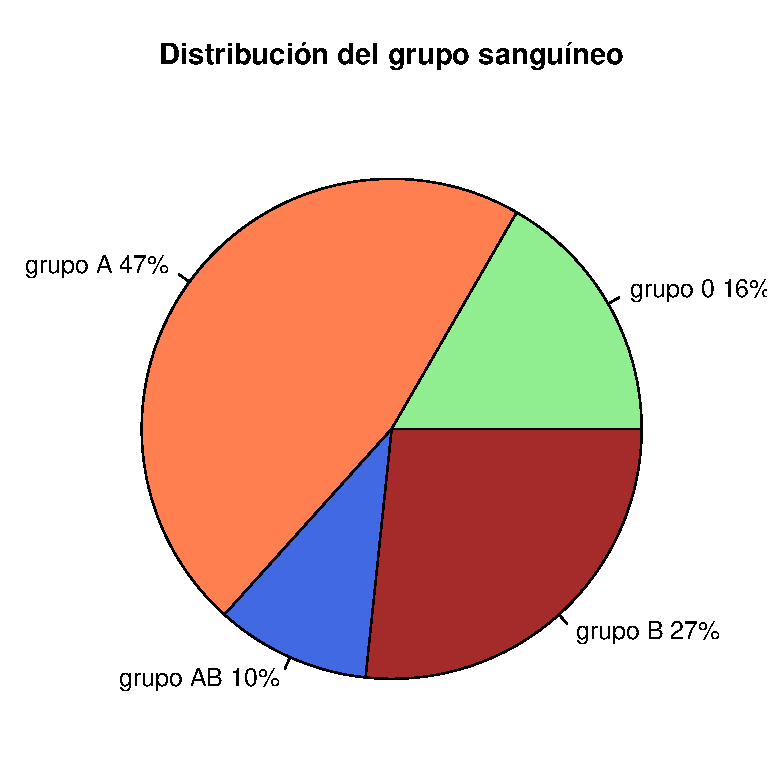
\includegraphics[scale=0.6]{img/descriptiva/diagrama_sectores_grupo_sanguineo}
\end{center}
\note{Tanto el diagrama de barras como el histograma se suele utilizar para variables cuantitativas ya que al tratarse
de un sistema cartesiano, los valores de las varibles deben ser numéricos. En el caso de los atributos el diagrama que
se suele utilizar es el diagrama de sectores, que consiste en un círculo dividido en sectores de área o ángulo
proporcional a la frecuencia correspondiente.

Para calcular el ángulo correspondiente a cada categoría, basta hacer una simple regla de tres, teniendo en cuenta que
los 360 grados de la circunferencia se corresponden con el tamaño muestral y calculando el ángulo correspondiente a
cada frecuencia. 

En este gráfico se pueden apreciar los sectores correspondientes a cada uno de los grupos sanguíneos en la muestra
anterior de 30 personas.}
\end{frame}


%---------------------------------------------------------------------slide----
\begin{frame}
\frametitle{Datos atípicos}
Uno de los principales problemas de las muestras son los datos atípicos. Los \structure{\textbf{datos atípicos}} son valores de la variable que se diferencian mucho del resto de los valores. 
\begin{center}
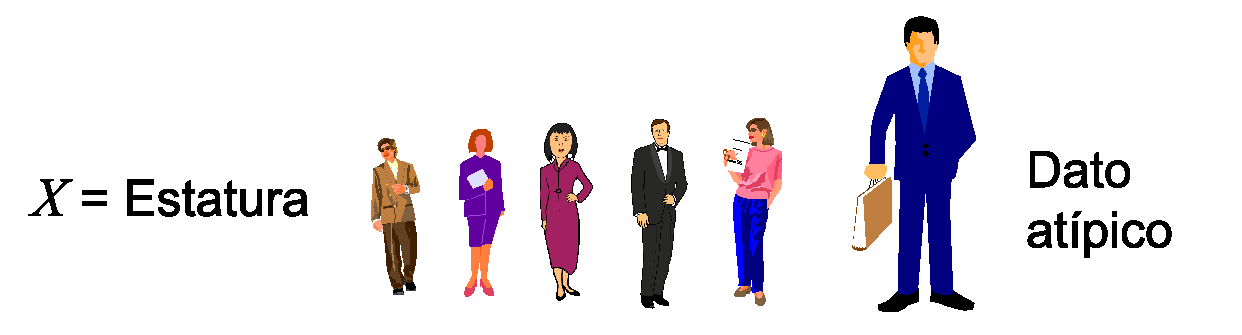
\includegraphics[scale=0.4]{img/descriptiva/dato_atipico}
\end{center}

Es muy importante detectar los datos atípicos antes de realizar cualquier análisis de los datos, pues \alert{\emph{suelen distorsionar los resultados}}. 

Aparecen siempre en los extremos de la distribución, aunque más adelante veremos un diagrama para detectarlos.

\note{Uno de los principales problemas que presentan las muestras es que pueden contener datos atípicos, es decir,
valores que se diferencian mucho del resto, bien porque son mucho mayores o menores que los demás.

Es muy importante detectar los datos atípicos antes de realizar cualquier análisis de los datos, 
pues suelen distorsionar las coclusiones extraidas de la muestra.

Para detectarlos hay que buscar en los extremos de la distribución, entre los valores menores y mayores, aunque más
adelante se mostrará un gráfico que permite detectarlos fácilmente.
}
\end{frame}


%---------------------------------------------------------------------slide----
\begin{frame}
\frametitle{Tratamiento de los datos atípicos}
Cuando trabajemos con muestras grandes, los datos atípicos tienen menor influencia y pueden dejarse en la muestra. 

Cuando trabajemos con muestras pequeñas tenemos varias opciones:
\begin{itemize}
\item Eliminarlo: Siempre que estemos seguros de que se trata de un error de medida.
\item Sustituirlo: Si se trata de un individuo real pero que no concuerda con el modelo de distribución de la población. En tal caso se suele reemplazar por el mayor o menor dato no atípico. 
\item Dejarlo: Si se trata de un individuo real aunque no concuerde con el modelo de distribución. En tal caso se suele modificar el modelo de distribución supuesto. 
\end{itemize}
\note{Si el tamaño de las muestra es grande, los datos atípicos tiene menor influencia que cuando el tamaño muestral es
pequeño. En este último caso conviene eliminar el dato atípico si se trata de un error de medida, sustituirlo por otro
valor más normal, que suele ser el mínimo o el máximo de los valores que se consideren normales, siempre que sea un
valor que corresponda a un individuo real pero que no se ajusta al modelo de distribución de la población, o bien
dejarlo y cambiar el modelo de distribución para que pueda explicar la existencia de esos valores atípicos.
}
\end{frame}


\subsection{Estadísticos muestrales}

%---------------------------------------------------------------------slide----
\begin{frame}
\frametitle{Estadísticos muestrales}
La tabla de frecuencias sintetiza la información de la variable estudiada en la muestra, pero en muchas ocasiones es insuficiente para describir determinados aspectos de la distribución.

Para describir adecuadamente el comportamiento de la variable se calculan unas medidas llamadas
\structure{\textbf{estadísticos muestrales}} que son indicadores de distintos aspectos de la distribución muestral.

Los estadísticos se clasifican en tres grupos:
\begin{description}
\item[Estadísticos de Posición:] Miden en torno a qué valores se agrupan los datos y cómo se reparten en la distribución.
\item[Estadísticos de Dispersión:] Miden la heterogeneidad de los datos.
\item[Estadísticos de Forma:] Miden aspectos de la forma que tiene la distribución de los datos,
como la simetría o el apuntamiento.
\end{description}  

\note{La tabla de frecuencias sintetiza la información de la variable estudiada en la muestra, pero en muchas
ocasiones resulta insuficiente para describir determinados aspectos de la distribución, como por ejemplo la
variabilidad entre los valores o los valores en torno a los cuales se agrupan la mayor parte de los individuos de la
muestra.

Para describir adecuadamente el comportamiento de la variable se calculan unas medidas llamadas
estadísticos muestrales que son indicadores de distintos aspectos de la distribución muestral.

Dependiendo del aspecto de las distribución que describen se clasifican en:
\begin{description}
\item[Estadísticos de Posición:] Miden en torno a qué valores se agrupan los datos y cómo se reparten a lo largo de la
distribución.
\item[Estadísticos de Dispersión:] Miden la heterogeneidad o variabilidad de los datos.
\item[Estadísticos de Forma:] Miden aspectos de la forma que tiene la distribución de los datos, como la simetría o el
apuntamiento.
\end{description}  
}
\end{frame}


\subsection{Estadísticos de posición}

%---------------------------------------------------------------------slide----
\begin{frame}
\frametitle{Estadísticos de posición}
Pueden ser de dos tipos:
\begin{description}
\item[Estadísticos de Tendencia Central:] Determinan valores alrededor de los cuales se agrupa la distribución. Estas
medidas suelen utilizarse como valores representativos de la muestra. Las más importantes son:
\begin{itemize}
\item Media aritmética
\item Mediana
\item Moda
\end{itemize}
\item [Otros estadísticos de Posición:] Dividen la distribución en partes con el mismo número de observaciones. Las más importantes son:
\begin{itemize}
\item Cuantiles: Cuartiles, Deciles, Percentiles.
\end{itemize}
\end{description}
\note{Veremos primero los estadísticos de posición, que se ocupan de dos tareas:
Por un lado, ver en torno a que valores se agrupan los valores de la muestra y qué valores son los más representativos
de la muestra. Estos son tres, la media, la mediana y la moda y se conocen como estadísticos de tendencia central.
Y por otro lado, ver cómo se reparten los datos a lo largo de la distribución. De esto se encargan los percentiles que
dividen la distribución en partes iguales.

Empezaremos viendo los estadísticos de tendencia central
}
\end{frame}


%---------------------------------------------------------------------slide----
\begin{frame}
\frametitle{Media aritmética}
\begin{definicion}[Media aritmética muestral $\bar{x}$]
La \emph{media aritmética muestral} de una variable $X$ es la suma de los valores observados en la muestra dividida por el tamaño muestral
\[
\bar{x} = \frac{\sum x_i}{n}
\]
\end{definicion}
A partir de la tabla de frecuencias puede calcularse como:
\[
\bar{x} &= \frac{\sum x_in_i}{n} = \sum x_i f_i
\]
En la mayoría de los casos, la media aritmética es la medida que mejor representa a la muestra. 
\begin{center}
\alert{\emph{¡Ojo! No puede calcularse para atributos.}}
\end{center}

\note{La media aritmética es, sin duda, el estadístico de tendencia central más conocido.
Se define como la suma de los valores observados en la muestra dividida por el tamaño muestral.

Si en lugar de la muestra tenemos la tabla de frecuencias, para calcular la media aritmética hay que sumar los
productos de cada valor por su frecuencia absoluta y dividir la suma entre el tamaño de la muestra, o bien directamente
sumando los productos de cada valor por su frecuencia relativa.

Algo que hay que advertir, es que, aunque la media aritmética es la medida de tendencia central más usada, no puede
calcularse para atributos, ya que las categorías no son números que pueden operarse artiméticamente.
}
\end{frame}


%---------------------------------------------------------------------slide----
\begin{frame}
\frametitle{Cálculo de la media aritmética}
\framesubtitle{Ejemplo con datos no agrupados}
En el ejemplo anterior del número de hijos tenemos 
\begin{align*}
\bar{x} &= \frac{1+2+4+2+2+2+3+2+1+1+0+2+2}{25}+\\
&+\frac{0+2+2+1+2+2+3+1+2+2+1+2}{25} = \frac{44}{25} = 1.76 \mbox{ hijos}.
\end{align*}
o bien, desde la tabla de frecuencias
\begin{center}
\setlength\arraycolsep{3mm}
\setlength\arrayrulewidth{0.5pt}
\begin{array}{rrrrr}
\hline
\multicolumn{1}{c}{x_i} & \multicolumn{1}{c}{n_i} & \multicolumn{1}{c}{f_i} & \multicolumn{1}{c}{x_in_i} & \multicolumn{1}{c}{x_if_i}\\
\hline
0 & 2 & 0.08 & 0 & 0\\
1 & 6 & 0.24 & 6 & 0.24\\
2 & 14 & 0.56 & 28 & 1.12\\
3 & 2  & 0.08 & 6 & 0.24\\
4 & 1 & 0.04 & 4 & 0.16 \\ 
\hline 
\sum & 25 & 1 & 44 & 1.76 \\
\hline
\end{array}
\end{center}
\[
\bar{x} = \frac{\sum x_in_i}{n} = \frac{44}{25}= 1.76 \qquad \bar{x}=\sum{x_if_i} = 1.76.
\]
Es decir, el número de hijos que mejor representa a la muestra es $1.76$ hijos.
\note{En el ejemplo del número de hijos en una muestra de 25 matrimonios, para calcular la media a partir de la
muestra, basta con sumar los hijos de cada matrimonio, 1 + 2 + 3, y así hasta el último, lo que da 44 hijos y dividirlo
por el número de matrimonios, 25, con lo que se obtiene 1.76 hijos de media.

Si en lugar de la muestra tenemos la tabla de frecuencias, entonces conviene construir una nueva columna donde se vayan
calculando los productos de cada valor por su frecuencia absoluta, es decir, 0 * 2 = 0 + 1 * 6 = 6, etc., luego sumar
todos estos productos, lo que de nuevo nos da 44 hijos y finalmente dividir la suma por el tamaño de la muestra que es
25, obteniendo de nuevo 1.76 hijos. La otra opción es construir otra columna donde se vayan calculando los productos de
cada valor por su frecuencia relativa, es decir, 0*0.08=0 + 1*0.24 = 0.24, etc. y finalmente sumar estos productos para
obtener, una vez más, 1.76 hijos de media.
}
\end{frame}


%---------------------------------------------------------------------slide----
\begin{frame}
\frametitle{Cálculo de la media aritmética}
\framesubtitle{Ejemplo con datos agrupados}
En el ejemplo anterior de las estaturas se tiene
\[
\bar{x} &= \frac{179+173+\cdots+187}{30} = 175.07 \mbox{ cm}.
\]
o bien, desde la tabla de frecuencias utilizando las marcas de clase:
\begin{center}
\setlength\arraycolsep{3mm}
\setlength\arrayrulewidth{0.5pt}
\begin{array}{rrrrrr}
\hline
\multicolumn{1}{c}{X} & \multicolumn{1}{c}{x_i} & \multicolumn{1}{c}{n_i} & \multicolumn{1}{c}{f_i} & \multicolumn{1}{c}{x_in_i} & \multicolumn{1}{c}{x_if_i}\\
\hline
(150,160] & 155 & 2 & 0.07 & 310 & 10.33\\
(160,170] & 165 & 8 & 0.27 & 1320 & 44.00\\
(170,180] & 175 & 11 & 0.36 & 1925 & 64.17\\
(180,190] & 185 & 7 & 0.23 & 1295 & 43.17\\
(190,200] & 195 & 2 & 0.07 & 390 & 13 \\ 
\hline  
\sum &  & 30 & 1 & 5240 & 174.67 \\
\hline
\end{array}
\end{center}
\[
\bar{x} = \frac{\sum x_in_i}{n} = \frac{5240}{30}= 174.67 \qquad \bar{x}=\sum{x_if_i} = 174.67.
\]
Al agrupar datos el cálculo de estadísticos desde la tabla puede diferir ligeramente del valor real obtenido directamente desde la muestra, ya que no se trabaja con los datos reales sino con los representantes de las clases.
\note{Cuando se trabaja con datos agrupados, el cálculo de la media aritmética a partir de la tabla de frecuencias,
cambia ligeramente, ya que ahora en lugar de valores se tienen intervalos. Lo se hace es tomar como representante de
cada clase el valor central, es decir, la marca de clase, y hacer los cálculos con ella. Por
ejemplo, el primer intervalo que va de 150 cm a 160 cm, su marca de clase es el centro que vale 155 cm, y entonces se
multiplica este valor por su frecuencia absoluta, que vale 2, dando 310 cm. Esto se repite para todos los valores, al
igual que antes, luego se suman los productos, obteniendo 5240 cm, y se divide por el tamaño de la muestra que era 30,
lo que da 174.67 cm de estatura media. 

También podríamos haber hecho el cálculo con las frecuencias relativas.
}
\end{frame}


%---------------------------------------------------------------------slide----
\begin{frame}
\frametitle{Media ponderada}
En algunos casos, los valores de la muestra no tienen la misma importancia. En este caso la media aritmética no es una
buena medida de representatividad ya que en ella todos los valores de la muestra tienen el mismo peso. En este caso es
mucho mejor utilizar otra medida de tendencia central conocida como media ponderada.


\begin{definicion}[Media ponderada muestral $\bar{x}_p$]
Dada una muestra de $n$ valores en la que cada valor $x_i$ tiene asociado un peso $p_i$, la \emph{media ponderada
muestral} de la variable $X$ es la suma de los productos de cada valor observado en la muestra por su peso, dividida
por la suma de todos los pesos
\[
\bar{x}_p = \frac{\sum x_ip_i}{\sum p_i}
\]
\end{definicion}
A partir de la tabla de frecuencias puede calcularse como:
\[
\bar{x}_p &= \frac{\sum x_ip_in_i}{\sum p_i}
\]

\note{En ocasiones, no todos los valores de la muestra tienen la misma importancia. En este caso la media aritmética
no es una buena medida de representatividad ya que en ella todos los valores tienen el mismo peso. En este caso es
mucho mejor utilizar otra medida de tendencia central conocida como media ponderada.

La media ponderada para una muestra de tamaño $n$ en la que cada valor $x_i$ tiene asociado un peso $p_i$ se define
como la suma de los productos de cada valor por su peso, dividida por la suma de todos los pesos. 

En el caso de estar trabajando desde la tabla de frecuencias, los productos de los valores por los pesos deben
multiplicarse también por la frecuencia absoluta de cada valor.
}
\end{frame}


%---------------------------------------------------------------------slide----
\begin{frame}
\frametitle{Cálculo de la media ponderada}
Supongase que un alumno quiere calcular la nota media de las asignaturas de un curso. 
\begin{center}
\begin{tabular}{lcc}
\hline
Asignatura & Créditos & Nota\\
\hline
Matemáticas & 6 & 5 \\
Lengua & 4 & 3 \\
Química & 8 & 6 \\
\hline 
\end{tabular}
\end{center}
La media aritmética vale
\[
\bar{x} = \frac{\sum x_i}{n} = \frac{5+3+6}{3}= 4.67 \text{ puntos},
\]
Sin embargo, esta nota no representa bien el rendimiento académico del alumno ya que en
ella han tenido igual peso todas las asignaturas, cuando la química debería tener más peso que la lengua al tener más
créditos.

Es más lógico calcular la media ponderada, tomando como pesos los créditos de cada asignatura:
\[
\bar{x}_p = \frac{\sum x_ip_i}{\sum p_i} = \frac{5\cdot 6+3\cdot 4+6\cdot 8}{6+4+8}= \frac{90}{18} = 5 \text{ puntos}.
\]

\note{Veamos un ejemplo. Supongamos que para evaluar el rendimiento académico de un alumno durante un curso queremos
calcular la nota media del curso a partir de las notas de todas las asignaturas. Las asignaturas cursadas han sido
matemáticas, de 6 créditos, que equivale a 60 horas de clase, donde ha sacado un 5, lengua, de 4 créditos, donde ha
sacado un 3 y química, de 8 créditos, y donde ha sacado un 6. 

Si se calcula la media aritmética, se obtiene una nota media de $4.67$ puntos, lo que supondría un suspenso. 

Ahora bien, esta nota no refleja bien el rendimiento del alumno ya que todas las notas no tienen el mismo peso. Por
ejemplo la química tiene el doble de créditos que la lengua, y por tanto, debería tener el doble de peso. 
En consecuencia, es mucho más acertado calcular la media ponderada tomando como pesos los créditos de las asignaturas.
Para calcularla multiplicamos la nota de cada asignatura por sus créditos, $5\cdot 6+3\cdot 4+6\cdot 8$, que vale 90 y
lo dividimos por la suma de los créditos, $6+4+8$, que vale 18, lo de da una nota media de 5.

Esta nota representa mucho mejor el rendimiento del alumno, y además ahora estaría aprobado.}
\end{frame}


%---------------------------------------------------------------------slide----
\begin{frame}
\frametitle{Mediana}
\begin{definicion}[Mediana muestral $Me$]
La \emph{mediana muestral} de una variable $X$ es el valor de la variable que, una vez ordenados los valores de la
muestra de menor a mayor, deja el mismo número de valores por debajo y por encima de él.
\end{definicion}

La mediana cumple $N_{Me}= n/2$ y  $F_{Me}= 0.5$.

El cálculo de la mediana se realiza de forma distinta según se hayan agrupado los datos o no.

\begin{center}
\alert{\emph{¡Ojo! No puede calcularse para atributos nominales.}}
\end{center}

\note{Otro estadístico de tendencia central bastante utilizado es la mediana, que se define como el valor que ocupa el
centro de la distribución, una vez ordenados los datos de menor a mayor.

Como está en el centro de la distribución, la mitad de los valores quedarán por debajo de ella y la otra mitad por
encima, y por tanto se cumple que la mediana tiene frecuencia absoluta acumulada n/2 o, lo que es lo mismo, frecuencia
relativa acumulada $0.5$.

La mediana resuelve en parte el problema de la media con los atributos, ya que puede calcularse para atributos
ordinales donde las categorías pueden ordenarse, pero no se puede calcular para atributos nominales.
}
\end{frame}


%---------------------------------------------------------------------slide----
\begin{frame}
\frametitle{Cálculo de la mediana con datos no agrupados}
Con datos no agrupados pueden darse varios casos:
\begin{itemize}
\item Tamaño muestral impar: La mediana es el valor que ocupa la posición $\frac{n+1}{2}$.
\item Tamaño muestral par: La mediana es la media de los valores que ocupan las posiciones $\frac{n}{2}$ y $\frac{n}{2}+1$.
\end{itemize}
\begin{center}
\includegraphics[scale=0.4]{img/descriptiva/mediana}
\end{center}
\note{Una vez ordenados los valores de la muestra de menor a mayor, el cálculo de la mediana con datos no agrupados,
depende de si el tamaño de la muestra es par o impar. Si es impar, entonces habrá un único valor central que ocupará la posición $\frac{n+1}{2}$ y dicho valor será la mediana.
Mientras que si el tamaño muestral es par, entonces habrá dos valores centrales, que ocuparan las posiciones
$\frac{n}{2}$ y $\frac{n}{2}+1$. Si estos valores son iguales, la mediana será ese valor, mientras que si son
distintos, la mediana estará entre los valores que ocupan estas posiciones y si puede se calculará su media aritmética.
}
\end{frame}


%---------------------------------------------------------------------slide----
\begin{frame}
\frametitle{Cálculo de la mediana}
\framesubtitle{Ejemplo con datos no agrupados}
En el ejemplo anterior del número de hijos, el tamaño muestral es 25, de manera que al ser impar se deben ordenar los
datos de menor a mayor y buscar el que ocupa la posición $\frac{25+1}{2} = 13$.
\[
0,0,1,1,1,1,1,1,2,2,2,2,\fbox{2},2,2,2,2,2,2,2,2,2,3,3,4
\]
y la mediana es 2 hijos.

Si se trabaja con la tabla de frecuencias, se debe buscar el primer valor cuya frecuencia absoluta acumulada iguala o
supera a 13, que es la posición que le corresponde a la mediana, o bien el primer valor cuya frecuencia relativa
acumulada iguala o supera a $0.5$:
\[
\setlength\arraycolsep{3mm}
\setlength\arrayrulewidth{0.5pt}
\begin{array}{rrrrr}
\hline
x_i & n_i & f_i & N_i & F_i\\
\hline
0 & 2 & 0.08 & 2 & 0.08\\
1 & 6 & 0.24 & 8 & 0.32\\
\rowcolor{coral} \fbox{2} & 14 & 0.56 & 22 & 0.88\\
3 & 2  & 0.08 & 24 & 0.96\\
4 & 1 & 0.04 & 25 & 1 \\ 
\hline 
\sum & 25 & 1 \\
\hline
\end{array}
\]

\note{Volviendo al ejemplo del número de hijos en una muestra de 25 matrimonios, para calcular la mediana, primero se
ordenan los datos de menor a mayor, y después se busca el valor centra, que en este caso, al ser un tamaño impar, es
único y ocupa la posición $\frac{25+1}{2}$ que vale 13. Contamos 1,2, hasta la 13 y observalos que el valor que aparece
es un 2. Luego la mediana es 2 hijos.

Para calcular la mediana a partir de la tabla de frecuencias, hay que buscar de nuevo el individuo que ocupa la
posición 13, y para ello se busca en la tabla el valor que tiene una frecuencia absoluta acumulada igual o mayor que 13.
En la tabla se puede observar que la primera frecuencia absoluta acumulada que iguala o supera al 13 es 22 y
corresponde al valor 2 que es la mediana.
}
\end{frame}


%---------------------------------------------------------------------slide----
\begin{frame}
\frametitle{Cálculo de la mediana con datos agrupados}
Con datos agrupados la mediana se calcula interpolando en el polígono de frecuencias absolutas acumuladas para el valor $n/2$.
\begin{center}
\scalebox{0.7}{\begin{pspicture}(0,-3.65375)(13,4)
\rput(1.9442188,-2.38625){\psaxes[linewidth=0.04,labels=none,ticksize=0.0958cm,dx=10.0cm,dy=6.0cm,Dx=10,Dy=5](0,0)(0,0)(10.01,6.01)}
\rput[c](7,-3.47625){$X$}
\rput{-270.0}(1.4,0.5359375){\rput(0.1621875,0.72375){Frecuencia Absoluta Acumulada $N_i$}}
\psline[linewidth=0.04,linecolor=blue](1.9642187,-2.38625)(3.9642189,-1.98625)(5.9642186,-0.38625)(7.9642186,1.81375)(9.964219,3.21375)(11.964219,3.61375)
\psline[linewidth=0.04,linecolor=orange,linestyle=dashed,dash=0.16cm 0.16cm](1.9642187,0.61375)(6.9,0.61375)(6.9,-2.38625)
\rput[r](1.6,0.62){$\dfrac{n}{2}$}
\rput[r](1.6,3.6){$n$}
\rput[c](7,-2.8){Mediana}
\end{pspicture}}
\end{center}
\note{Cuando se trabaja con datos agrupados en clases, la mediana se calcula de forma aproximada, interpolando en el
polígono de frecuencias acumuladas para el valor $n/2$. 

La interpolación consiste en proyectar sobre el polígono la frecuencia $n/2$ y ver a qué altura del eje de abscisas
corta al polígono de frecuencias. Dicho valor es la mediana.
}
\end{frame}


%---------------------------------------------------------------------slide----
\begin{frame}
\frametitle{Interpolación en el polígono de frecuencias absolutas acumuladas}
\begin{center}
\scalebox{1}{\begin{pspicture}(-1,-0.5)(9,5)
\psaxes[arrows=->,ticks=none,labels=none](0,0)(0,0)(6,5)
\pspolygon[fillcolor=royalblue1,fillstyle=solid,linestyle=none](1,1)(5,4)(5,1)
\uncover<2-3>{\pspolygon[fillcolor=coral,fillstyle=solid,linestyle=none](1,1)(3.67,3)(3.67,1)}
\psline[linestyle=dashed](0,1)(5,1)
\psline[linestyle=dashed](0,4)(5,4)
\psline[linestyle=dashed](1,0)(1,1)
\psline[linestyle=dashed](5,0)(5,4)
\psline[linecolor=blue](1,1)(5,4)
\psarc(1,1){0.3}{0}{35}
\rput[r](-0.1,1){$N_{i-1}$}
\rput[r](-0.1,4){$N_{i}$}
\rput[t](1,-0.1){$l_{i-1}$}
\rput[t](5,-0.1){$l_{i}$}
\rput[l](1.4,1.2){$\alpha$}
\rput[l](6,3){\color{royalblue1} $\tg(\alpha) = \dfrac{N_i-N_{i-1}}{l_i-l_{i-1}}$}
\uncover<2->{
\rput[r](-0.1,3){$n/2$}
\psline[linestyle=dashed](0,3)(3.67,3)
\psline[linestyle=dashed](3.67,0)(3.67,3)
\rput[t](3.67,-0.1){$Me$}
%\pspolygon[fillcolor=coral,fillstyle=solid,linestyle=none](1,1)(3.67,3)(3.67,1)
\rput[l](6,2){\color{coral}$\tg(\alpha) = \dfrac{n/2-N_{i-1}}{Me-l_{i-1}}$}
}
\end{pspicture}}
\end{center}

\uncover<3->{
\[
Me = l_{i-1}+\frac{n/2 - N_{i-1}}{N_i-N_{i-1}}(l_i-l_{i-1}) = l_{i-1}+\frac{n/2-N_{i-1}}{n_i}a_i
\]
}

\note{La interpolación en realidad consiste en una razón de semejanza de triángulos. 

En primer lugar se identifica el intervalo en el que cae la mediana, mirando en la columna de frecuencias acumuladas de
la tabla de frecuencias, de igual modo a como se hace para datos no agrupados. Una vez identificado el intervalo, se
toma el segmento del polígono de frecuencias acumuladas que corresponde a dicho intervalo. Supongamos que dicho
intervalo tiene límite inferior $l_{i-1}$ y límite superior $l_i$, y que parte de una frecuencia absoluta acumulada
$N_{i-1}$ y llega a una frecuencia absoluta acumulada $N_{i}$. Este segmento define un triángulo rectángulo de ángulo
$\alpha$ cuya tangente es el cateto opuesto, que vale $N_i-N_{i-1}$ entre el cateto contiguo, que es precisamente la
amplitud del intervalo $l_i-l_{i-1}$.

Por otro lado, si proyectamos la frecuencia corresondiente a la media $n/2$ sobre el polígono, en el punto de corte
aparecería la mediana, de manera se se tiene otro triángulo rectángulo más pequeño que es semejante al anterior al
compartir el mismo ángulo $\alpha$. Al igual que antes, la tangente de este ángulo será el cateto opuesto, que ahora
vale $n/2-N_i$ entre el cateto contiguo que ahora vale $Me-l_{i-1}$. 

Puesto que se trata del mismo ángulo, su tangente es la misma y se pueden igual ambas expresiones, dando lugar a una
ecuación conde la única incógnita es la mediana. Despejandola, se obtiene la fórmula para calcular la mediana.
}
\end{frame}


%---------------------------------------------------------------------slide----
\begin{frame}
\frametitle{Cálculo de la mediana}
\framesubtitle{Ejemplo con datos agrupados}
En el ejemplo de las estaturas $n/2 =
30/2 = 15$. Si miramos en el polígono de frecuencias acumuladas comprobamos que
la mediana caerá en el intervalo $(170,180]$.
\begin{center}
\scalebox{0.7}{\begin{pspicture}(0,-3.65375)(13,4)
\rput(10,0){\setlength\arraycolsep{3mm}
\setlength\arrayrulewidth{0.5pt}
\begin{array}{rrr}
\hline
\multicolumn{1}{c}{x_i} & \multicolumn{1}{c}{n_i} & \multicolumn{1}{c}{N_i} \\
\hline
(150,160] & 2 & 2 \\
(160,170] & 8 & 10 \\
\rowcolor{coral} (170,180] & 11 & 21 \\
(180,190] & 7  & 28 \\
(190,200] & 2  & 30 \\ 
\hline 
\end{array}}
\rput(1.9442188,-2.38625){\psaxes[linewidth=0.04,ticksize=0.10583333cm,dx=2.0cm,dy=1.0cm,Dx=10,Dy=5,Ox=150](0,0)(0,0)(10.01,6)}
\rput(6.7046876,-3.47625){$X = $ Estatura}
\rput{-270.0}(0.6721875,0.5359375){\rput(0.1621875,0.72375){Frecuencia Absoluta Acumulada $N_i$}}
\uncover<2->{\pspolygon[fillcolor=royalblue1,fillstyle=solid,linestyle=none](5.9642186,-0.38625)(7.9642186,1.81375)(7.9642186,-0.38625)}
\psline[linewidth=0.04,linecolor=blue](1.9642187,-2.38625)(3.9642189,-1.98625)(5.9642186,-0.38625)(7.9642186,1.81375)(9.964219,3.21375)(11.964219,3.61375)
\uncover<2->{
\psline[linewidth=0.04,linecolor=gray,linestyle=dashed,dash=0.16cm 0.16cm](1.9642187,-0.38625)(5.9642186,-0.38625)(5.9642186,-2.38625)(5.9842186,-2.40625) 
\psline[linewidth=0.04,linecolor=gray,linestyle=dashed,dash=0.16cm 0.16cm](1.9642187,1.81375)(7.9642186,1.81375)(7.9642186,-2.38625)(7.9842186,-2.40625)
\psline[linewidth=0.04,linecolor=orange,linestyle=dashed,dash=0.16cm 0.16cm](1.9642187,0.61375)(6.9642186,0.61375)(6.9642186,-2.38625)(6.9842186,-2.40625)
\rput[r](1.2,0.62){$\dfrac{n}{2}=$}
\rput[c](7,-2.8){$Me$}
}
\end{pspicture}}
\end{center}
\note{Veamos un ejemplo de interpolación para calcular la mediana de la muestra de estaturas. Mirando en la tabla de
frecuencias se observa que el primer intervalo con una frecuencia igual o mayor que $n/2=30/2=15$ es el que va de 170
cm a 180 cm, así que se toma el trozo del polígono de frecuencias absolutas acumuladas corresondiente a este intervalo.
}
\end{frame}


%---------------------------------------------------------------------slide----
\begin{frame}
\frametitle{Interpolación en el polígono de frecuencias absolutas acumuladas}
\begin{center}
\scalebox{1}{\psset{unit=1}
\begin{pspicture}(-1,-0.5)(9,5)
\psaxes[arrows=->,ticks=none,labels=none](0,0)(0,0)(6,5)
\pspolygon[fillcolor=royalblue1,fillstyle=solid,linestyle=none](1,1)(5,4)(5,1)
\only<2-3>{\pspolygon[fillcolor=coral,fillstyle=solid,linestyle=none](1,1)(2.85,2.4)(2.85,1)}
\psline[linestyle=dashed](0,1)(5,1)
\psline[linestyle=dashed](0,4)(5,4)
\psline[linestyle=dashed](1,0)(1,1)
\psline[linestyle=dashed](5,0)(5,4)
\psline[linecolor=blue](1,1)(5,4)
\psarc(1,1){0.3}{0}{35}
\rput[r](-0.1,1){$10$}
\rput[r](-0.1,4){$21$}
\rput[t](1,-0.1){$170$}
\rput[t](5,-0.1){$180$}
\rput[l](1.4,1.2){$\alpha$}
\rput[l](6,3){\color{royalblue1} $\tg(\alpha) = \dfrac{21-10}{180-170}$}
\uncover<2->{
\rput[r](-0.1,2.4){$n/2=15$}
\psline[linestyle=dashed](0,2.4)(2.85,2.4)
\psline[linestyle=dashed](2.85,0)(2.85,2.4)
\rput[t](2.75,-0.1){$Me$}
%\pspolygon[fillcolor=coral,fillstyle=solid,linestyle=none](1,1)(3.67,3)(3.67,1)
\rput[l](6,2){\color{coral}$\tg(\alpha) = \dfrac{15-10}{Me-170}$}
}
\end{pspicture}}
\end{center}

\uncover<3->{
\[
Med = 170+\frac{15 - 10}{21-10}(180-170) = 170+\frac{5}{11}10 = 174.54
\]
}

\note{Si nos fijamos en el triángulo grande, la tangente de $\alpha$ vale $21-10$ que es el cateto opuesto, entre
$180-170$ que es el cateto contiguo, mientras que si nos fijamos en el triángulo pequeño que aparece al proyectar $15$
sobre el polígono, se tiene que la tangente de $\alpha$ vale $15-10$ que es cateto opuesto entre $Me-170$ que es el
cateto contiguo. Igualando ambas expresiones y despejando la mediana se obtiene $174.54$ cm que es la estatura mediana.

Una comprobación que conviene hacer siempre es ver que el valor obtenido cae efectivamente dentro del intervalo de
interpolación.}
\end{frame}


%---------------------------------------------------------------------slide----
\begin{frame}
\frametitle{Moda}
\begin{definicion}[Moda muestral $Mo$]
La \emph{moda muestral} de una variable $X$ es el valor de la variable más frecuente en la muestra.
\end{definicion}
Con datos agrupados se toma como clase modal la clase con mayor frecuencia en la muestra.

En ocasiones puede haber más de una moda.
\begin{center}
\includegraphics[scale=0.5]{img/descriptiva/moda}
\end{center}
\note{El último estadístico de tendencia central que veremos se llama moda, y viene a suplir las carencias de la media
y mediana, que no podían calcularse para atributos nominales.

La moda se define como el valor más frecuente en la muestra, y puede ocurrir que en algunas distribuciones haya más de
una moda.
}
\end{frame}


%---------------------------------------------------------------------slide----
\begin{frame}
\frametitle{Cálculo de la moda}
En el ejemplo del número de hijos puede verse fácilmente en la tabla de frecuencias que la moda es $Mo = 2$ hijos. 
\begin{center}
\setlength\arraycolsep{3mm}
\setlength\arrayrulewidth{0.5pt}
\begin{array}{rr}
\hline
\multicolumn{1}{c}{x_i} & \multicolumn{1}{c}{n_i} \\
\hline
0 & 2 \\
1 & 6 \\
\rowcolor{coral} \fbox{2} & 14 \\
3 & 2  \\
4 & 1 \\ 
\hline 
\end{array}
\end{center}
Y en el ejemplo de las estaturas también puede verse en la tabla de frecuencias que la clase modal es $Mo=(170,180]$.
\begin{center}
\setlength\arraycolsep{3mm}
\setlength\arrayrulewidth{0.5pt}
\begin{array}{rr}
\hline
\multicolumn{1}{c}{x_i} & \multicolumn{1}{c}{n_i} \\
\hline
(150,160] & 2 \\
(160,170] & 8 \\
\rowcolor{coral} \fbox{(170,180]} & 11 \\
(180,190] & 7 \\
(190,200] & 2 \\ 
\hline 
\end{array}
\end{center}
\note{La moda es el estadístico más sencillo de calcular pues sólo hay que fijarse en la columna de frecuencias
absolutas de la tabla de frecuencias, buscar la mayor y ver a qué valor le corresponde.

En el ejemplo del número de hijos, la mayor frecuencia es 14, que le corresponde al 2, de manera que la moda es 2 hijos.

En el ejemplo de las estaturas, la mayor frecuencia es 11, que le corresponde al intervalo $(170,180]$ que es el
intervalo modal.}
\end{frame}


%---------------------------------------------------------------------slide----
\begin{frame}
\frametitle{¿Qué estadístico de tendencia central usar?}
En general, siempre que puedan calcularse conviene tomarlas en el siguiente orden:
\begin{enumerate}
\item Media. La media utiliza más información que el resto ya que para calcularla se tiene en cuenta la magnitud de los datos.
\item Mediana. La mediana utiliza menos información que la media, pero más que la moda, ya que para calcularla se tiene
en cuenta el orden de los datos.
\item Moda. La moda es la que menos información utiliza ya que para calcularla sólo se tienen en cuenta las frecuencias absolutas.
\end{enumerate}
Pero, ¡ojo! la media también es muy sensible a los datos atípicos, así que, tampoco debemos perder de vista la mediana.

Por ejemplo, consideremos la siguiente muestra del número de hijos de 7 matrimonios:
\begin{center}
0, 0, 1, 1, 2, 2, 15

$\bar{x}=3$ hijos \quad y \quad $Me=1$ hijos

\emph{¿Qué representante de la muestra tomarías?}
\end{center}

\note{Hemos visto tres estadístico de tendencia central, de manera que surge la pregunta de cuál usar en el caso de que
puedan calcularse los tres. 

En principio, siempre que pueda calcularse se tomará la media, pues es la medida que más información utiliza de la
muestra al tener en cuenta la magnitud de los datos. Si no puede calcularse la media, se utilizará la mediana, que
aunque no tiene en cuenta la magnitud de los valores, al menos si tiene en cuenta el orden entre ellos. Y finalmente,
si no se pueden calcular ninguna de las dos, se tomará la moda que únicamente tiene en cuenta las frecuencias de los
valores.

Una excepción a esta regla es cuando en la muestra haya datos atípicos, ya que la media es muy sensible a datos
atípicos, mientras que la mediana no lo es apenas. Si nos fijamos en esta pequeña muestra con el número de hijos de 7
matrimonios, con un matrimonio que es claramente atípico por tener 15 hijos, podemos ver que la media vale 3 hijos,
mientras que sin el dato atípico valdría 1 hijo. Es decir, la media se ve muy alterada por el dato atípico. Si embargo
la mediana vale 1 hijo tanto con el dato atípico como sin el. En estas circunstancias es mejor utilizar la mediana como
medida de representatividad.}
\end{frame}


%---------------------------------------------------------------------slide----
\begin{frame}
\frametitle{Cuantiles}
Son valores de la variable que dividen la distribución, supuesta ordenada de menor a mayor, en partes que contienen el mismo número de datos.

Los más utilizados son:
\begin{description}
\item[Cuartiles:] Dividen la distribución en 4 partes iguales.\\
Hay tres cuartiles: $C_1$ (25\% acumulado) , $C_2$ (50\% acumulado), $C_3$ (75\% acumulado). 
\item[Deciles:] Dividen la distribución en 10 partes iguales.\\
Hay 9 deciles: $D_1$ (10\% acumulado) ,\ldots, $D_9$ (90\% acumulado).
\item[Percentiles:] Dividen la distribución en 100 partes iguales.\\
Hay 99 percentiles: $P_1$ (1\% acumulado),\ldots, $P_{99}$ (99\% acumulado).
\end{description}

\note{Una vez vistas las medidas de tendencia central, pasamos al resto de medidas de posición que son los cuantiles y
que dividen la muestra en partes iguales. Existen distintos tipos:
\begin{description}
\item[Cuartiles:] Dividen la distribución en 4 partes iguales.\\
Hay tres cuartiles: $C_1$ (25\% acumulado) , $C_2$ (50\% acumulado), $C_3$ (75\% acumulado). \\
Obsérvese que la mediana coincide con el segundo cuartil.
\item[Deciles:] Dividen la distribución en 10 partes iguales.\\
Hay 9 deciles: $D_1$ (10\% acumulado) ,\ldots, $D_9$ (90\% acumulado).
\item[Percentiles:] Dividen la distribución en 100 partes iguales.\\
Hay 99 percentiles: $P_1$ (1\% acumulado),\ldots, $P_{99}$ (99\% acumulado).
\end{description}

Obsérvese la correspondencia que hay entre algunos cuantiles, como por ejemplo el primer cuartil que se corresponde con
el pertencil 25 o el tercer cuartil que se corresponde con el percentil 75. 
}
\end{frame}


%---------------------------------------------------------------------slide----
\begin{frame}
\frametitle{Cálculo de los cuantiles}
Los cuantiles se calculan de forma similar a la mediana. Por ejemplo, en el caso de los cuartiles se buscan los valores que tienen frecuencias absolutas acumuladas $n/4$ (primer cuartil), $n/2$ (segundo cuartil) y $3n/4$ (tercer cuartil) y si se trata de datos agrupados se interpola sobre el polígono de frecuencias acumuladas.
\begin{center}
\begin{center}
\scalebox{0.7}{
\begin{pspicture}(0,-3.65375)(13,4)
\rput(1.9442188,-2.38625){\psaxes[linewidth=0.04,labels=none,ticksize=0.0958cm,dx=10.0cm,dy=6.0cm,Dx=10,Dy=5](0,0)(0,0)(10.01,6.01)}
\rput[c](7,-3.47625){$X$}
\rput{-270.0}(1.4,0.5359375){\rput(0.1621875,0.72375){Frecuencia Absoluta Acumulada $N_i$}}
\psline[linewidth=0.04,linecolor=blue](1.9642187,-2.38625)(3.9642189,-1.98625)(5.9642186,-0.38625)(7.9642186,1.81375)(9.964219,3.21375)(11.964219,3.61375)
\psline[linewidth=0.04,linecolor=orange,linestyle=dashed,dash=0.16cm 0.16cm](1.9642187,0.61375)(6.9,0.61375)(6.9,-2.38625)
\psline[linewidth=0.04,linecolor=orange,linestyle=dashed,dash=0.16cm 0.16cm](1.9642187,2.11375)(8.3,2.11375)(8.3,-2.38625)
\psline[linewidth=0.04,linecolor=orange,linestyle=dashed,dash=0.16cm 0.16cm](1.9642187,-0.88625)(5.3,-0.88625)(5.3,-2.38625)
\rput[r](1.6,2.12){$\dfrac{3n}{4}$}
\rput[r](1.6,0.62){$\dfrac{n}{2}$}
\rput[r](1.6,-0.88){$\dfrac{n}{4}$}
\rput[r](1.6,3.6){$n$}
\rput[c](5.3,-2.8){$C_1$}
\rput[c](6.9,-2.8){$C_2$}
\rput[c](8.3,-2.8){$C_3$}
\end{pspicture}}
\end{center}
\end{center}
\note{Los cuantiles se calculan, al igual que la mediana, interpolando sobre el polígono de frecuencias absolutas
acumuladas. Por ejemplo, para los cuartiles, proyectando la frecuencia absloluta acumulada del primer cuartil, que es
$n/4$, se obtiene el primer cuartil, proyectando $n/2$ se obtiene el segundo cuartil, y proyectando $3n/4$ se obtiene
el primer cuartil, y lo mismo para los otros cuantiles.}
\end{frame}


%---------------------------------------------------------------------slide----
\begin{frame}
\frametitle{Cálculo de los cuantiles}
\framesubtitle{Ejemplo con datos no agrupados}
En el ejemplo anterior del número de hijos se tenían la siguientes frecuencias relativas acumuladas
\begin{center}
\setlength\arraycolsep{3mm}
\setlength\arrayrulewidth{0.5pt}
\begin{array}{rr}
\hline
\multicolumn{1}{c}{x_i} & \multicolumn{1}{c}{F_i} \\
\hline
0 & 0.08\\
1 & 0.32\\
2 & 0.88\\
3 & 0.96\\
4 & 1\\ 
\hline
\end{array}
\end{center}
\begin{align*}
F_{C_1}=0.25 &\Rightarrow C_1 = 1 \text{ hijos},\\
F_{C_2}=0.5 &\Rightarrow C_2 = 2 \text{ hijos},\\
F_{C_3}=0.75 &\Rightarrow C_3 = 2 \text{ hijos},\\
F_{D_3}=0.3 &\Rightarrow D_3 = 1 \text{ hijos},\\
F_{P_{92}}=0.92 &\Rightarrow P_{92} = 3 \text{ hijos}.\\
\end{align*}
\note{Los cuantiles se calculan de forma similara a la mediana a partir de las frecuencias acumuladas correspondientes a cada uno de ellos.

En el ejemplo del número de hijos donde se tenían las frecuencias relativas acumuladas que aparecen en esta tabla, para calcular el primer
cuartil se parte de su frecuencia relativa acumulada que es $0.25$ ya que hasta el primer cuartil se tienen acumulados el 25\% de los
individuos y se busca en la tabla el primer valor cuya frecuencia relativa acumulada es igual o superior a $0.25$, que en este caso es 1
hijo, ya que su frecuencia relativa acumulada es $0.32$ que supera a $0.25$ mientras que la frecuencia relativa acumulada del 0 no llega a
$0.25$. Del mismo modo, el cuartil segundo, cuya frecuencia relativa acumulada es $0.5$, es 2 hijos y el tercer cuartil, con frecuencia
relativa acumulada $0.75$ también es 2 hijos.

Para el decil tercero, su frecuencia relativa acumulada es $0.3$, y procediendo como para los cuartiles, se observa que el primer valor con
frecuencia relativa acumulada igual o superior a $0.3$ es 1 hijo.

Finalmente, para el percentil 92, su frecuencia relativa acumulada es $0.92$ y el primer valor con frecuencia relativa acumulada igual o
superior a este valor es 3 hijos.}
\end{frame}


\subsection{Estadísticos de dispersión}
%---------------------------------------------------------------------slide----
\begin{frame}
\frametitle{Estadísticos de dispersión}
Recogen información respecto a la heterogeneidad de la variable y a la concentración de sus valores en torno a algún valor central.


Para las variables cuantitativas, las más empleadas son:
\begin{itemize}
\item Recorrido.
\item Rango Intercuartílico.
\item Varianza.
\item Desviación Típica.
\item Coeficiente de Variación.
\end{itemize}
\note{Uno de los aspectos más importantes de una muestra es la variabilidad de los datos, que también se conoce como
dispersión de la muestra. Veremos hasta 5 estadísticos para describir la dispersión:
\begin{itemize}
\item Recorrido.
\item Rango Intercuartílico.
\item Varianza.
\item Desviación Típica.
\item Coeficiente de Variación.
\end{itemize}
}
\end{frame}


%---------------------------------------------------------------------slide----
\begin{frame}
\frametitle{Recorrido}
\begin{definicion}[Recorrido muestral $Re$]
El \emph{recorrido muestral} de una variable $X$ se define como la diferencia entre el máximo y el mínimo de los valores en la muestra.
\[Re = \max_{x_i} -\min_{x_i}\]
\end{definicion}
El recorrido da una idea de la máxima variación que hay entre los datos muestrales. No obstante, es muy sensible a datos atípicos ya que suelen aparecer justo en los extremos de la distribución, por lo que no se suele utilizar mucho.

\begin{center}
\scalebox{1} % Change this value to rescale the drawing.
{
\begin{pspicture}(-1,-1)(9,1)
\psline[linewidth=0.04cm]{|-|}(0,0)(8,0)
\rput[t](0,-0.2){$\min$}
\rput[t](8,-0.2){$\max$}
\psline[linecolor=orange]{<->}(0,0.5)(8,0.5)
\rput[b](4,0.7){$Re$}
\end{pspicture}}
\end{center}
\note{El recorrido es el estadístico de dispersión más natural ya que consiste en medir la distancia que va del mayor
al menor de los valores y se calcula restándolos. 

Cuanto mayor sea el recorrido, mayor dispersión habrá en la muestra.

El principal problema que presenta el recorrido es que es muy sensible a los datos atípicos, ya que estos precisamente
aparecen en los extremos de la distribución. }
\end{frame}


%---------------------------------------------------------------------slide----
\begin{frame}
\frametitle{Rango intercuartílico}
Para evitar el problema de los datos atípicos en el recorrido, se puede utilizar el primer y tercer cuartil en lugar del mínimo y el máximo.
\begin{definicion}[Rango intercuartílico muestral $RI$]
El \emph{rango intercuartílico muestral} de una variable $X$ se define como la diferencia entre el tercer y el primer
cuartil de la muestra. \[RI = C_3 -C_1\]
\end{definicion}
El rango intercuartílico da una idea de la variación que hay en el 50\% de los datos centrales. 

\begin{center}
\scalebox{1} % Change this value to rescale the drawing.
{
\begin{pspicture}(-1,-1)(9,1)
\psline[linewidth=0.04cm]{|-|}(0,0)(8,0)
\rput[t](0,-0.2){$\min$}
\rput[t](8,-0.2){$\max$}
\psline[linewidth=0.04cm]{|-|}(2,0)(4,0)
\psline[linewidth=0.04cm]{|-|}(0,0)(6,0)
\rput[t](2,-0.2){$C_1$}
\rput[t](4,-0.2){$C_2$}
\rput[t](6,-0.2){$C_3$}
\rput[b]](1,0.1){$25\%$}
\rput[b]](3,0.1){$25\%$}
\rput[b]](5,0.1){$25\%$}
\rput[b]](7,0.1){$25\%$}
\psline[linecolor=orange]{<->}(2,0.5)(6,0.5)
\rput[b](4,0.7){$RI$}
\end{pspicture}}
\end{center}
\note{Para evitar el problema que tiene el Recorrido con los datos atípicos, se suele utilizar el Rango
Intercuartílico, que utiliza la misma idea del Recorrido pero midiendo la distancia que va del tercer al primer
cuartil. 

Si recordamos, los cuartiles dividen la distribución en 4 partes iguales, de manera que entre el primer y el tercer
cuartil estan el 50\% de los datos centrales de la distribución, y quedarían exlucidos el 25\% de valores menores y el
25\% de valores mayores, donde posiblemente estarían los datos atípicos. 

Por tanto el Rango Intercuartílico mide la dispersión central de la muestra, de manera que cuanto mayor sea, más
dispersión central tendrá la muestra, aunque siempre hay que tener en cuenta las unidades de la variable al
interpretarlo. }
\end{frame}


%---------------------------------------------------------------------slide----
\begin{frame}
\frametitle{Diagrama de caja y bigotes}
La dispersión de una variable suele representarse gráficamente mediante un \structure{\textbf{diagrama de caja y bigotes}}, que consiste en una caja sobre un eje $X$ donde el borde inferior de la caja es el primer cuartil, y el borde superior el tercer cuartil, y por tanto, la anchura de la caja es el rango intercuartílico.
En ocasiones también se representa el segundo cuartil con una línea que divide la caja. 

También se utiliza para detectar los valores atípicos mediante unos segmentos (bigotes) que salen de los extremos de la caja y que marcan el intervalo de normalidad de los datos.
\note{La dispersión de la muestra se representa a menudo mediante un diagrama de caja y bigotes, que como su propio
nombre indica, consiste en una caja sobre un eje $X$ donde el borde inferior de la caja es el primer cuartil, y el
borde superior el tercer cuartil, y por tanto, la anchura de la caja, por tanto, es el rango intercuartílico. 
En ocasiones también se representa el segundo cuartil con una línea que divide la caja.

También se utiliza para detectar los valores atípicos de la muestra mediante unos segmentos llamados bigotes que
salen de los extremos de la caja y que marcan el intervalo de normalidad de los datos.
}
\end{frame}


%---------------------------------------------------------------------slide----
\begin{frame}
\frametitle{Diagrama de caja y bigotes}
\framesubtitle{Ejemplo con pesos de recién nacidos}
\begin{center}
\scalebox{0.75}{%% Input file name: diagrama_caja.fig
%% FIG version: 3.2
%% Orientation: Landscape
%% Justification: Flush Left
%% Units: Inches
%% Paper size: A4
%% Magnification: 100.0
%% Resolution: 1200ppi

\begin{pspicture}(7.41cm,3.48cm)(17.02cm,13.45cm)
\psset{unit=0.8cm}
%%
%% Depth: 2147483647
%%
\newrgbcolor{mycolor0}{1.00 0.50 0.31}\definecolor{mycolor0}{rgb}{1.00,0.50,0.31}
%%
%% Depth: 100
%%
\psset{linestyle=dashed,linewidth=0.03175}
\psline(11.84,10.88)(14.04,10.88)
\psline(18.00,10.88)(15.81,10.88)
\psset{linestyle=solid,fillstyle=solid,fillcolor=mycolor0}
\pspolygon(14.04,9.25)(14.04,12.51)(15.81,12.51)(15.81,9.25)(14.04,9.25)
\psline(11.84,10.06)(11.84,11.69)
\psline(18.00,10.06)(18.00,11.69)
\qdisk(10.61,10.88){0.1}
\qdisk(19.94,10.88){0.1}
\psset{linestyle=solid,linewidth=0.0635,linecolor=black,fillstyle=none}
\psline(14.83,9.25)(14.83,12.51)
\psset{fillstyle=none}
\psline(10.75,6.47)(19.94,6.47)
\psline(10.75,6.47)(10.75,6.26)
\psline(12.59,6.47)(12.59,6.26)
\psline(14.43,6.47)(14.43,6.26)
\psline(16.26,6.47)(16.26,6.26)
\psline(18.10,6.47)(18.10,6.26)
\psline(19.94,6.47)(19.94,6.26)
\rput(10.75,5.71){2.0}
\rput(12.59,5.71){2.5}
\rput(14.43,5.71){3.0}
\rput(16.26,5.71){3.5}
\rput(18.10,5.71){4.0}
\rput(19.94,5.71){4.5}
\rput(15.27,15.99){Diagrama de caja y bigotes del peso de recien nacidos}
\rput(15.27,4.86){Peso (Kg)}
\psline(10.23,6.47)(20.31,6.47)(20.31,15.28)(10.23,15.28)(10.23,6.47)
\rput[l](13.84,8.74){$C_1$}
\rput[l](14.58,8.74){$C_2$}
\rput[l](15.68,8.74){$C_3$}
\rput[l]{90}(10.65,11.35){Dato atípico}
\end{pspicture}
%% End
}
\end{center}
\note{Aquí podemos ver un ejemplo de un diagrama de caja y bigotes para una muestra de pesos de recién nacidos. 
El borde inferior de la caja corresponde al primer cuartil, que es aproximadamente $2.8$ Kg, el borde superior
corresponde al tercer cuartil, que vale aproximadamente $3.4$ Kg, de manera que el ancho de la caja es el rango
intercuartílico, y vale aproximadamente $0.6$ Kg, lo que indica una dispersión central baja, teniendo en cuenta que
los pesos de los recién nacidos se suelen mover en unas unidades que van de 1 a 4 Kg, más o menos.

De la caja salen dos sementos, que son los bigotes, el inferior llega aproximadamente hasta $2.3$ Kg y el superior
hasta $4$ Kg, delimitando el intervalo de normalidad de los datos, de manera que cualquier niño que pese menos de $2.3$
Kg o más de $4$ Kg será un individuo atípico. De hecho en esta muestra aparecen dos pesos atípicos que aparecen
marcados por puntos, uno que corresponde a un niño con 2 Kg de peso, y otro que corresponde a otro niño con 4.5 Kg de
peso.}
\end{frame}


%---------------------------------------------------------------------slide----
\begin{frame}
\frametitle{Construcción del diagrama de caja y bigotes}
\begin{enumerate}
\item Calcular los cuartiles.
\item Dibujar una caja de manera que el extremo inferior caiga sobre el primer cuartil y el extremo superior sobre el tercer cuartil.
\item Dividir la caja con una línea que caiga sobre el segundo cuartil. 
\item Para los bigotes inicialmente se determina la posición de los puntos denominados \emph{vallas} $v_1$ y $v_2$ restando y sumando respectivamente a primer y tercer cuartil $1.5$ veces el rango intercuartílico $RI$:
\begin{align*}
v_1&=C_1-1.5RI\\
v_2&=C_3+1.5RI
\end{align*}
A partir de las vallas se buscan los valores $b_1$, que es el mínimo valor de la muestra mayor o igual que  $v_1$,
y $b_2$, que es máximo valor de la muestra menor o igual que $v_2$. Para el bigote inferior se dibuja un segmento
desde el borde inferior de la caja hasta $b_1$ y para el superior se dibuja un segmento desde el borde superior de la caja hasta $b_2$.
\item Finalmente, si en la muestra hay algún dato por debajo de $v_1$ o por encima de $v_2$ se dibuja un punto sobre dicho valor. 
\end{enumerate}
\note{Para construcir el diagrama de cajas, hay que seguir los siguientes pasos:
\begin{enumerate}
\item Calcular los cuartiles.
\item Dibujar una caja de manera que el extremo inferior caiga sobre el primer cuartil y el extremo superior sobre el tercer cuartil.
\item Dividir la caja con una línea que caiga sobre el segundo cuartil. 
\item Para los bigotes inicialmente se determina la posición de los puntos denominados \emph{vallas} $v_1$ y $v_2$ restando y sumando respectivamente a primer y tercer cuartil $1.5$ veces el rango intercuartílico $RI$:
\begin{align*}
v_1&=C_1-1.5RI\\
v_2&=C_3+1.5RI
\end{align*}
A partir de las vallas se buscan los valores $b_1$, que es mínimo valor de la muestra mayor o igual que $v_1$,
y $b_2$ es máximo valor de la muestra menor o igual que $v_2$. Para el bigote inferior se dibuja un segmento
desde el borde inferior de la caja hasta $b_1$ y para el superior se dibuja un segmento desde el borde superior de la caja hasta $b_2$.
\item Finalmente, si en la muestra hay algún dato por debajo de $v_1$ o por encima de $v_2$ se dibuja un punto sobre dicho valor. 
\end{enumerate}}
\end{frame}


%---------------------------------------------------------------------slide----
\begin{frame}
\frametitle{Construcción del diagrama de caja y bigotes}
\framesubtitle{Ejemplo del número de hijos}
\begin{enumerate}
\uncover<2->{\item Calcular los cuartiles: $C_1=1$ hijos} \uncover<3->{y $C_3=2$ hijos.}
\uncover<4->{\item Dibujar la caja.}
\uncover<5->{\item Calcular las vallas: $v_1=1-1.5*1=-0.5$ y $v_2=2+1.5*1=3.5$.}
\uncover<6->{\item Dibujar los bigotes: $b_1=0$ hijos} \uncover<7->{y $b_1=3$ hijos.} 
\uncover<8->{\item Dibujar los datos atípicos: 4 hijos.} 
\end{enumerate}
\begin{center}
\scalebox{0.65}{%% Input file name: descriptiva/diagrama_caja_hijos.fig
%% FIG version: 3.2
%% Orientation: Landscape
%% Justification: Flush Left
%% Units: Inches
%% Paper size: A4
%% Magnification: 100.0
%% Resolution: 1200ppi

\begin{pspicture}(7.77cm,3.48cm)(16.66cm,12.45cm)
\psset{unit=0.8cm}
%%
%% Depth: 2147483647
%%
\newrgbcolor{mycolor0}{1.00 0.50 0.31}\definecolor{mycolor0}{rgb}{1.00,0.50,0.31}
%%
%% Depth: 100
%%
\psset{linestyle=solid,linecolor=black,fillstyle=none}
\psline(10.61,6.47)(19.94,6.47)
\psline(10.61,6.47)(10.61,6.26)
\psline(12.94,6.47)(12.94,6.26)
\psline(15.27,6.47)(15.27,6.26)
\psline(17.60,6.47)(17.60,6.26)
\psline(19.94,6.47)(19.94,6.26)
\rput(10.61,5.71){0}
\rput(12.94,5.71){1}
\rput(15.27,5.71){2}
\rput(17.60,5.71){3}
\rput(19.94,5.71){4}
\rput(15.27,15.49){Diagrama de caja y bigotes del número de hijos}
\rput(15.27,4.86){Número de hijos}
\psline(10.23,6.47)(20.31,6.47)(20.31,14.88)(10.23,14.88)(10.23,6.47)
\uncover<2->{
\psline(12.94,9.25)(12.94,12.51)
\rput(12.94,8.74){$C_1$}
}
\uncover<3->{
\psline(15.27,9.25)(15.27,12.51)
\rput(15.27,8.74){$C_3$}
}
\uncover<4->{
\psset{fillstyle=solid,fillcolor=mycolor0}
\pspolygon(12.94,9.25)(12.94,12.51)(15.27,12.51)(15.27,9.25)(12.94,9.25)
}
\uncover<6->{
\psline(10.61,10.06)(10.61,11.69)
\psset{linestyle=dashed}
\psline(10.61,10.88)(12.94,10.88)
}
\uncover<7->{
\psset{linestyle=solid}
\psline(17.60,10.06)(17.60,11.69)
\psset{linestyle=dashed}
\psline(17.60,10.88)(15.27,10.88)
}
\uncover<8->{
\psset{linestyle=solid,linecolor=black,fillstyle=solid,fillcolor=black}
\pscircle(19.94,10.88){0.1}
}
\end{pspicture}
%% End
}
\end{center}
\note{Veamos cómo construir el diagrama de caja y bigotes para el ejemplo del número de hijos:
\begin{enumerate}
\item Primero se calcula el primer cuartil que era 1 hijo y se dibuja el borde inferior de la caja. Después se calcula el tercer cuartil
que era 3 hijos y se dibuja el borde superior de la caja.
\item Una vez dibujados el borde inferior y superior de la caja se acaba de dibujar esta. 
\item También se suele dibujar el cuartil segundo mediante una linea que divide la caja, pero en este ejemplo, al coincidir el cuartil
segundo con el tercero, no se dibuja. 
\item A continuación se calcula el rango intercuartílico que era 2-1=1 hijo y con el se calcula la valla inferior $v_1$ restandole al primer
cuartil $1.5$ veces el rango intercuartílico, lo que nos da $-0.5$ hijos, y la valla superior $v_2$ sumandole al tercer cuartil $1.5$ veces
el rango intercuartílico, lo que nos da $3.5$ hijos.
\item Luego se calculan los extremos de los bigotes. El extremo del bigote inferior es $0$ hijos, ya que es el mínimo valor de la muestra
por encima de la valla inferior que valía $-0.5$, y el bigote superiror es $3$ hijos, ya que es el máximo valor de la muestra por debajo de
la valla superior que valía $3.5$ hijos. 
\item Finalmente se dibujan los datos atípicos. Por debajo de la valla inferior no hay ningún valor en la muestra, pero por encima de la
valla superior si hay una familia con 4 hijos, que se trata, por tanto, de una familia atípica y si se dibuja un punto en diagrama sobre
dicho valor. 
\end{enumerate}}
\end{frame}


%---------------------------------------------------------------------slide----
\begin{frame}
\frametitle{Desviaciones respecto de la media}
Otra forma de medir la variabilidad de una variable es estudiar la concentración de los valores en torno a algún estadístico de tendencia central como por ejemplo la media. 

Para ello se suele medir la distancia de cada valor a la media. A ese valor se le llama
\structure{\textbf{desviación respecto de la media.}}
\begin{center}
\scalebox{1} % Change this value to rescale the drawing.
{
\begin{pspicture}(-1,-0.5)(7,1.5)
\psline(0,0)(6,0)
\psdots(1,0)(5,0)
\psdot[linecolor=orange](3,0)
\rput[t](3,-0.2){$\bar{x}$}
\rput[t](1,-0.2){$x_i$}
\rput[t](5,-0.2){$x_j$}
\psline[linecolor=orange]{<->}(1,0.5)(3,0.5)
\rput[b](2,0.7){$x_i-\bar{x}$}
\rput[b](2,1.2){\scriptsize Desviación $-$}
\psline[linecolor=orange]{<->}(3,0.5)(5,0.5)
\rput[b](4,0.7){$x_j-\bar{x}$}
\rput[b](4,1.2){\scriptsize Desviación $+$}
\end{pspicture}}
\end{center}

Si las desviaciones son grandes la media no será tan representativa como cuando la desviaciones sean pequeñas.
\begin{center}
\scalebox{1} % Change this value to rescale the drawing.
{
\begin{pspicture}(-1,-0.5)(7,1.6)
\psline(0,1.6)(6,1.6)
\psdots(0.1,1.6)(0.2,1.6)(0.4,1.6)(0.5,1.6)(0.8,1.6)(5,1.6)(5.3,1.6)(5.4,1.6)(5.7,1.6)(5.8,1.6)
\psdot[linecolor=orange](3,1.6)
\rput[t](3,1.4){$\bar{x}$}
\rput[l](-2.5,1.6){\footnotesize Más dispersión}
\rput[l](6.3,1.6){\footnotesize $\bar x$ menos representativa}
\psline(0,0.2)(6,0.2)
\psdots(1.5,0.2)(2,0.2)(2.2,0.2)(2.5,0.2)(2.8,0.2)(3.3,0.2)(3.5,0.2)(3.9,0.2)(4.1,0.2)(4.4,0.2)
\psdot[linecolor=orange](3,0.2)
\rput[t](3,0){$\bar{x}$}
\rput[l](-2.5,0.2){\footnotesize Menos dispersión}
\rput[l](6.3,0.2){\footnotesize $\bar x$ más representativa}
\end{pspicture}}

\emph{¿En qué muestra es más representativa la media?}
\end{center}

\note{Otra forma de medir la variabilidad de una variable es estudiar la concentración de los valores en torno a algún estadístico de
tendencia central, como por ejemplo la media.  

Para ello se suele medir la distancia que hay de cada valor a la media, que se conoce como desviación respecto a la media. Cuando el valor
sea mayor que la media su desviación será positiva, y cuando sea menor que la media su desviación será negativa. 

Resulta evidente que si las desviaciones son grandes, entonces los datos estarán bastante alejados de la media y por tanto la media no será
tan representativa de la muestra como cuando los valores estén concentrados en torno a la media y sus desviaciones sean pequeñas.

Aquí tenemos dos casos en los que la dispersión con respecto a la media es mayor en el primer caso es mayor que en el segundo, de manera que
la media será más representativa en el último caso que en el primero.}
\end{frame}


%---------------------------------------------------------------------slide----
\begin{frame}
\frametitle{Varianza y desviación típica}
\begin{definicion}[Varianza $s^2$]
La \emph{varianza muestral} de una variable $X$ se define como el promedio del cuadrado de las desviaciones de los
valores de la muestra respecto de la media muestral.
\[
s^2 = \frac{\sum (x_i-\bar x)^2n_i}{n} = \sum (x_i-\bar x)^2f_i
\]
\end{definicion}
También puede calcularse de manera más sencilla mediante la fórmula
\[
s^2 = \frac{\sum x_i^2n_i}{n} -\bar x^2= \sum x_i^2f_i-\bar x^2
\]
La varianza tiene las unidades de la variable al cuadrado, por lo que para facilitar su interpretación se suele utilizar su raíz cuadrada:
\begin{definicion}[Desviación típica $s$]
La \emph{desviación típica muestral} de una variable $X$ se define como la raíz cuadrada positiva de su varianza muestral.
\[
s = +\sqrt{s^2}
\]
\end{definicion}

\note{A partir de las desviaciones con respecto a la media surge un estadístico conocido como varianza, que se representa como $s^2$ y que
se calcula sumando las desviaciones de los valores a la media elevadas al cuadrado y dividiendo la suma por el tamaño de la muestra. El
hecho de considerar los cuadrados es para sumar siempre magnitudes positivas, ya que de lo contrario las desviaciones positivas se
compensarían con las negativas. Además, siempre que se trabaje desde la tabla, hay que multiplicar cada desviación al cuadrado por su
correspondiente frecuencia absoluta.

Si se desarrolla el cuadrado de cada desviación y se simplifica, se llega a otra expresión equivalente para calcular la varianza que
consiste en sumar los cuadrados de los valores multiplicados por su frecuencia absoluta, dividir la suma por el tamaño de la muestra y al
resultado restarle la media al cuadrado. Esta fórmula es un poco más sencilla de calcular y será la que utilizaremos casi siempre.

Como la varianza se calcula a partir de las desviaciones, cuando estas sean grandes, la varianza será grande, lo que indicará gran
dispersión y cuando estas sean pequeñas la varianza también será pequeña indicando poca dispersión. El único inconveniente es que la
varianza tiene unidades al cuadrado, lo cual dificulta su interpretación.

Para evitar este problema se suele tomar la raíz cuadrada de la varianza que se conoce como desviación típica y que también sirve para
medir la dispersión de los datos con respecto a la media, pero ahora con la ventaja de tener las mismas unidades que la variable.}
\end{frame}


%---------------------------------------------------------------------slide----
\begin{frame}
\frametitle{Interpretación de la varianza y la desviación típica}
Tanto la varianza como la desviación típica sirven para cuantificar la dispersión de los datos en torno a la media. 
%Si la dispersión es grande la media será menos representativa de la muestra que si la dispersión es pequeña.
\begin{center}
\includegraphics[scale=0.4]{img/descriptiva/interpretacion_varianza}

%\emph{¿En qué caso es más representativa la media?}
\end{center}

\note{Tanto la varianza como la desviación típica sirven para cuantificar la dispersión de los datos en torno a la media. Si la dispersion
con respecto a la media es pequeña, los individuos se parecerán bastante a la media y esta será más representativa que cuando los
individuos no se parezcana ella y la dispersión con respecto a la media sea mayor.}
\end{frame}


%---------------------------------------------------------------------slide----
\begin{frame}
\frametitle{Cálculo de la varianza y la desviación típica}
\framesubtitle{Ejemplo con datos no agrupados}
Para el número de hijos se puede calcular la varianza a partir de la tabla de frecuencias añadiendo una columna con los
cuadrados de los valores:
\begin{center}
\setlength\arraycolsep{3mm}
\setlength\arrayrulewidth{0.5pt}
\begin{array}{rrr}
\hline
\multicolumn{1}{c}{x_i} & \multicolumn{1}{c}{n_i} & \multicolumn{1}{c}{x_i^2n_i} \\
\hline
0 & 2 & 0 \\
1 & 6 & 6 \\
2 & 14 & 56\\
3 & 2  & 18\\
4 & 1 & 16 \\ 
\hline 
\sum & 25 & 96 \\
\hline
\end{array}
\end{center}
\[
s^2 = \frac{\sum x_i^2n_i}{n}-\bar x^2 = \frac{96}{25}-1.76^2= 0.7424 \mbox{ hijos}^2.
\]
Y la desviación típica es $s=\sqrt{0.7424} = 0.8616$ hijos.

Comparado este valor con el recorrido, que va de 0 a 4 hijos se observa que no es demasiado grande por lo que se puede concluir que no hay
mucha dispersión y en consecuencia la media de $1.76$ hijos representa bien a los matrimonios de la muestra.

\note{En el ejemplo del número de hijos, para calcular al varianza conviene añadir una nueva columna a la tabla donde se calculen los
productos de los cuadrados de los valores por sus frecuencias absolutas: 0 evado al cuadrado y por su frecuencia absoluta que es 2, da 0, 1
elevado al cuadrado y por su frecuencia absoluta que es 6, que da 6, y así sucesivamente. Después hay que sumar los valores de esta
columna y dividirlos por el tamaño de la muestra que era 25. Finalmente al cociente se le resta el valor de la media que era $1.76$
elevada al cuadrado, lo que nos da 0.7424 hijos al cuadrado.

Si sacamos la raíz cuadrada se obtiene una desviación típica de 0.8616 hijos, que no es un valor grande comparado con el recorrido de la
variable que va de 0 a 4 hijos, por lo que se puede concluir que la muestra no tiene mucha dispersión y por tanto la media de
$1.76$ hijos representa muy bien a los matrimonios de la muestra.}
\end{frame}


%---------------------------------------------------------------------slide----
\begin{frame}
\frametitle{Cálculo de la varianza y la desviación típica}
\framesubtitle{Ejemplo con datos agrupados}
En el ejemplo de las estaturas, al ser datos agrupados, el cálculo se realiza igual que antes pero tomando como valores de la variable las
marcas de clase. 
\begin{center}
\setlength\arraycolsep{3mm}
\setlength\arrayrulewidth{0.5pt}
\begin{array}{rrrr}
\hline
\multicolumn{1}{c}{X} & \multicolumn{1}{c}{x_i} & \multicolumn{1}{c}{n_i} & \multicolumn{1}{c}{x_i^2n_i} \\
\hline
(150,160] & 155 & 2 & 48050\\
(160,170] & 165 & 8 & 217800\\
(170,180] & 175 & 11 & 336875\\
(180,190] & 185 & 7 & 239575\\
(190,200] & 195 & 2 & 76050\\ 
\hline 
\sum &  & 30 & 918350 \\
\hline
\end{array}
\end{center}
\[
s^2 = \frac{\sum x_i^2n_i}{n}-\bar x^2 = \frac{918350}{30}-174.67^2= 102.06 \mbox{ cm}^2.
\]
Y la desviación típica es $s=\sqrt{102.06} = 10.1$ cm.

Este valor es bastante pequeño, comparado con el recorrido de la variable, que va de 150 a 200 cm, por lo que la variable tiene poca
dispersión y en consecuencia su media es muy representativa.

\note{En el ejemplo de las estaturas, como se habían agrupado los datos, como valores se tomarán las
marcas de clases, es decir, 155 elevado al cuadrado y por su frecuencia absoluta que es 2, lo que nos da 48050, y así sucesivamente. Después
hay que sumar los valores de esta columna y dividirlos por el tamaño de la muestra que era 30. Finalmente al cociente se le resta el valor
de la media que era $174.67$ elevada al cuadrado, lo que nos da 102.06 cm al cuadrado.

Si sacamos la raíz cuadrada se obtiene una desviación típica de 10.1 cm, que es un valor pequeño comparado con el recorrido de la variable
que va de 150 a 200 cm, por lo que se puede concluir que la muestra tiene poca dispersión y por tanto la media representa muy bien al resto
de individuos de la muestra.}
\end{frame}


%---------------------------------------------------------------------slide----
\begin{frame}
\frametitle{Coeficiente de variación}
Tanto la varianza como la desviación típica tienen unidades y eso dificulta a veces su interpretación y su comparación.

Afortunadamente es fácil definir a partir de ellas una medida de dispersión adimensional que es más fácil de interpretar.
\begin{definicion}[Coeficiente de variación muestral $cv$]
El \emph{coeficiente de variación muestral} de una variable $X$ se define como el cociente entre su desviación típica muestral y el valor absoluto de su media muestral.
\[
cv = \frac{s}{|\bar x|}
\]
\end{definicion}
El coeficiente de variación muestral mide la dispersión relativa de los valores de la muestra en torno a la media muestral.
 
Como no tiene unidades, es muy sencillo de interpretar: Cuanto mayor sea, mayor será la dispersión y menos
representativa será la media.

También se utiliza para comparar la dispersión entre muestras distintas incluso si las variables tienen unidades diferentes.
\begin{center}
\alert{\emph{¡Ojo! No tiene sentido cuando la media muestral vale 0 o valores próximos.}}
\end{center}

\note{Tanto la varianza como la desviación típica tienen unidades lo que dificulta a veces su interpretación.

Afortunadamente es fácil definir a partir de ellas una medida de dispersión adimensional que es más fácil de interpretar.

El coeficiente de variación muestral, que se representa mediante cv, se defiene como el cociente entre la desviación típica y el valor
absoluto de la media.

Como tanto la desviación típica como la media tienen las unidades de la variable, al hacer su cociente las unidades desaparecen y se obtiene
una medida adimensional que resulta más sencilla de interpretar. 

Al estar dividido por el valor absoluto de la media, el coeficiente de variación mide la dispersión relativa de los valores de la muestra
en torno a la media muestral, y como en el numerador está la desviación típica, cuanto mayor sea esta, mayor será el coeficiente de
variación y por tanto mayor será la dispersión relativa de la variable en torno a la media.

Una de las principales utilidades del coeficiente de variación es que, precisamente por no tener unidades, permite la comparación de la
dispersión de muestras distintas, incluso si son de variables con distintas unidades. 

El único problema de este estadístico es que no vale cuando la media muestral vale 0 o próxima a 0, ya que al estar en el denominador,
obtendríamos valores muy grandes.}
\end{frame}


%---------------------------------------------------------------------slide----
\begin{frame}
\frametitle{Coeficiente de variación}
\framesubtitle{Ejemplo}
En el caso del número de hijos, como $\bar x=1.76$ hijos y $s=0.8616$ hijos, se tiene que el coefiente de variación vale
\[
cv = \frac{s}{|\bar x|} = \frac{0.8616}{|1.76|} = 0.49.
\]
En el caso de las estaturas, como $\bar x=174.67$ cm y $s=10.1$ cm, se tiene que el coeficiente de variación vale 
\[
cv = \frac{s}{|\bar x|} = \frac{10.1}{|174.67|} = 0.06.
\]
Como se puede observar la dispersión relativa en la muestra de estaturas es mucho menor que en la del número de hijos, por lo que la media
de las estaturas será más representativa que la media del número de hijos. 
\end{frame}


\subsection{Estadísticos de forma}
%---------------------------------------------------------------------slide----
\begin{frame}
\frametitle{Estadísticos de forma}
Son medidas que tratan de caracterizar aspectos de la forma de la distribución de una muestra.

Los aspectos más relevantes son:
\begin{description}
\item[Simetría:] Miden la simetría de la distribución de frecuencias en torno a la media.\\
El estadístico más utilizado es el \emph{Coeficiente de Asimetría de Fisher}.
\item[Apuntamiento:] Miden el apuntamiento de la distribución de frecuencias.\\
El estadístico más utilizado es el \emph{Coeficiente de Apuntamiento o Curtosis}.
\end{description}
\note{Los estadísticos de forma se encargan de describir, como su propio nombre indica, la forma que tiene la distribución de valores en la
muestra, en particular se estudian dos aspectos que son la asímetría y el apuntamiento.}
\end{frame}


%---------------------------------------------------------------------slide----
\begin{frame}
\frametitle{Coeficiente de asimetría}
\begin{definicion}[Coeficiente de asimetría muestral $g_1$]
El \emph{coeficiente de asimetría muestral} de una variable $X$ se define como el promedio de las desviaciones de los
valores de la muestra respecto de la media muestral, elevadas al cubo, dividido por la desviación típica al cubo. \[g_1
= \frac{\sum (x_i-\bar x)^3 n_i/n}{s^3} = \frac{\sum (x_i-\bar x)^3 f_i}{s^3}\]
\end{definicion}
El coeficiente de asimetría muestral mide el grado de simetría de los valores de la muestra con respecto a la media muestral, de manera que:
\begin{itemize}
\item $g_1=0$ indica que hay el mismo número de valores a la derecha y a la izquierda de la media (simétrica).
\item $g_1<0$ indica que la mayoría de los valores son mayores que la media (asimétrica a la izquierda).
\item $g_1>0$ indica que la mayoría de los valores son menores que la media (asimétrica a la derecha).
\end{itemize}

\note{La simetría con respecto a la media tiene que ver con la ubicación de los valores a un lado y otro de la media, cuántos valores hay
por encima y cuántos por debajo, y cómo están de alejados.

El coeficiente de asimetría muestral, que se representa $g_1$ se define, como la suma del producto de las desviaciones de los valores de la
muestra a la media muestral elevadas al cubo por su frecuencia absoluta, dividida por el tamaño de la muestra, y a su vez todo dividido
por la desviación típica al cubo.

Como las desviaciones elevadas al cubo tienen las unidades de la variable al cubo y la desviación típica elevada al cubo también tiene las
unidades de la variable al cubo, al realizar el cociente las unidades se cancelan y por tanto el coeficiente de asimetría es una medida
adimensional que mide el grado de asimetría de los valores de la muestra con respecto a la media, de manera que:
\begin{itemize}
\item $g_1=0$ indica que hay el mismo número de valores a la derecha y a la izquierda de la media y por tanto la distribución es simétrica.
\item $g_1<0$ indica que la mayoría de los valores son mayores que la media y entonces se dice que la distribución es asimétrica hacia la
izquierda.
\item $g_1>0$ indica que la mayoría de los valores son menores que la media y entonces se dice que la distribución es asimétrica hacia la
derecha.
\end{itemize}
}
\end{frame}


%---------------------------------------------------------------------slide----
\begin{frame}
\frametitle{Coeficiente de asimetría}
\framesubtitle{Ejemplo de distribución simétrica}
\begin{center}
\scalebox{0.8}{%% Input file name: distribucion_simetrica.fig
%% FIG version: 3.2
%% Orientation: Landscape
%% Justification: Flush Left
%% Units: Inches
%% Paper size: A4
%% Magnification: 100.0
%% Resolution: 1200ppi
%% Include the following in the preamble:
%% \usepackage{textcomp}
%% End

\begin{pspicture}(5.91cm,3.25cm)(17.37cm,13.10cm)
\psset{unit=0.8cm}
%%
%% Depth: 2147483647
%%
\newrgbcolor{mycolor0}{1.00 0.50 0.31}\definecolor{mycolor0}{rgb}{1.00,0.50,0.31}
%%
%% Depth: 100
%%
\rput[l](13.59,15.54){Distribución simétrica \alert{$g_1=0$}}
\rput{90}(9.68,10.89){Frecuencia relativa}
\psset{linestyle=solid,linewidth=0.03175,linecolor=black,fillstyle=none}
\psline(11.04,7.07)(11.04,14.71)
\psline(11.04,7.07)(10.83,7.07)
\psline(11.04,8.98)(10.83,8.98)
\psline(11.04,10.89)(10.83,10.89)
\psline(11.04,12.80)(10.83,12.80)
\psline(11.04,14.71)(10.83,14.71)
\rput{90}(10.53,7.07){0.0}
\rput{90}(10.53,8.98){0.1}
\rput{90}(10.53,10.89){0.2}
\rput{90}(10.53,12.80){0.3}
\rput{90}(10.53,14.71){0.4}
\psset{fillstyle=solid,fillcolor=mycolor0}
\pspolygon(10.74,7.07)(10.74,7.07)(11.42,7.07)(11.42,7.07)(10.74,7.07)
\pspolygon(11.42,7.07)(11.42,7.11)(12.09,7.11)(12.09,7.07)(11.42,7.07)
\pspolygon(12.09,7.07)(12.09,7.25)(12.76,7.25)(12.76,7.07)(12.09,7.07)
\pspolygon(12.76,7.07)(12.76,7.69)(13.43,7.69)(13.43,7.07)(12.76,7.07)
\pspolygon(13.43,7.07)(13.43,8.75)(14.10,8.75)(14.10,7.07)(13.43,7.07)
\pspolygon(14.10,7.07)(14.10,10.56)(14.77,10.56)(14.77,7.07)(14.10,7.07)
\pspolygon(14.77,7.07)(14.77,12.83)(15.45,12.83)(15.45,7.07)(14.77,7.07)
\pspolygon(15.45,7.07)(15.45,14.38)(16.12,14.38)(16.12,7.07)(15.45,7.07)
\pspolygon(16.12,7.07)(16.12,14.36)(16.79,14.36)(16.79,7.07)(16.12,7.07)
\pspolygon(16.79,7.07)(16.79,12.80)(17.46,12.80)(17.46,7.07)(16.79,7.07)
\pspolygon(17.46,7.07)(17.46,10.58)(18.14,10.58)(18.14,7.07)(17.46,7.07)
\pspolygon(18.14,7.07)(18.14,8.75)(18.81,8.75)(18.81,7.07)(18.14,7.07)
\pspolygon(18.81,7.07)(18.81,7.70)(19.48,7.70)(19.48,7.07)(18.81,7.07)
\pspolygon(19.48,7.07)(19.48,7.26)(20.15,7.26)(20.15,7.07)(19.48,7.07)
\pspolygon(20.15,7.07)(20.15,7.11)(20.82,7.11)(20.82,7.07)(20.15,7.07)
\pspolygon(20.82,7.07)(20.82,7.07)(21.20,7.07)(21.20,7.07)(20.82,7.07)
\rput[l](16.03,6.5){$\bar x$}
\psset{linewidth=0.0635,fillstyle=none}
\psline(16.12,4.58)(16.12,5.76)
\psset{linestyle=dashed,linewidth=0.03175}
\psline(13.48,5.17)(15.46,5.17)
\psline(18.75,5.17)(16.78,5.17)
\psset{linestyle=solid}
\psline(13.48,4.88)(13.48,5.47)
\psline(18.75,4.88)(18.75,5.47)
\psline(15.46,4.58)(15.46,5.76)(16.78,5.76)(16.78,4.58)(15.46,4.58)
\end{pspicture}
%% End
}
\end{center}
\note{Aquí tenemos el histograma de una distribución simétrica. Como puede observarse, la media queda justo en el centro de la
distribución, coincidiendo con la mediana y existe el mismo número de barras y con la misma frecuencia a un lado y a otro de la media.}
\end{frame}


%---------------------------------------------------------------------slide----
\begin{frame}
\frametitle{Coeficiente de asimetría}
\framesubtitle{Ejemplo de distribución asimétrica hacia la izquierda}
\begin{center}
\scalebox{0.8}{%% Input file name: distribucion_asimetrica_izquierda.fig
%% FIG version: 3.2
%% Orientation: Landscape
%% Justification: Flush Left
%% Units: Inches
%% Paper size: A4
%% Magnification: 100.0
%% Resolution: 1200ppi
%% Include the following in the preamble:
%% \usepackage{textcomp}
%% End

\begin{pspicture}(5.91cm,3.25cm)(17.07cm,13.10cm)
\psset{unit=0.8cm}
%%
%% Depth: 2147483647
%%
\newrgbcolor{mycolor0}{1.00 0.50 0.31}\definecolor{mycolor0}{rgb}{1.00,0.50,0.31}
%%
%% Depth: 100
%%
\rput[l](12.07,15.54){Distribución asimétrica a la izquierda \alert{$g_1<0$}}
\rput{90}(9.68,10.89){Frecuencia relativa}
\psset{linestyle=solid,linewidth=0.03175,linecolor=black,fillstyle=none}
\psline(11.04,7.07)(11.04,14.71)
\psline(11.04,7.07)(10.83,7.07)
\psline(11.04,8.34)(10.83,8.34)
\psline(11.04,9.61)(10.83,9.61)
\psline(11.04,10.89)(10.83,10.89)
\psline(11.04,12.16)(10.83,12.16)
\psline(11.04,13.44)(10.83,13.44)
\psline(11.04,14.71)(10.83,14.71)
\rput{90}(10.53,7.07){0.00}
\rput{90}(10.53,8.34){0.02}
\rput{90}(10.53,9.61){0.04}
\rput{90}(10.53,10.89){0.06}
\rput{90}(10.53,12.16){0.08}
\rput{90}(10.53,13.44){0.10}
\rput{90}(10.53,14.71){0.12}
\psset{fillstyle=solid,fillcolor=mycolor0}
\pspolygon(10.79,7.07)(10.79,7.07)(11.42,7.07)(11.42,7.07)(10.79,7.07)
\pspolygon(11.42,7.07)(11.42,7.08)(12.04,7.08)(12.04,7.07)(11.42,7.07)
\pspolygon(12.04,7.07)(12.04,7.08)(12.67,7.08)(12.67,7.07)(12.04,7.07)
\pspolygon(12.67,7.07)(12.67,7.11)(13.30,7.11)(13.30,7.07)(12.67,7.07)
\pspolygon(13.30,7.07)(13.30,7.15)(13.92,7.15)(13.92,7.07)(13.30,7.07)
\pspolygon(13.92,7.07)(13.92,7.24)(14.55,7.24)(14.55,7.07)(13.92,7.07)
\pspolygon(14.55,7.07)(14.55,7.42)(15.18,7.42)(15.18,7.07)(14.55,7.07)
\pspolygon(15.18,7.07)(15.18,7.75)(15.81,7.75)(15.81,7.07)(15.18,7.07)
\pspolygon(15.81,7.07)(15.81,8.32)(16.43,8.32)(16.43,7.07)(15.81,7.07)
\pspolygon(16.43,7.07)(16.43,9.29)(17.06,9.29)(17.06,7.07)(16.43,7.07)
\pspolygon(17.06,7.07)(17.06,10.70)(17.69,10.70)(17.69,7.07)(17.06,7.07)
\pspolygon(17.69,7.07)(17.69,12.43)(18.31,12.43)(18.31,7.07)(17.69,7.07)
\pspolygon(18.31,7.07)(18.31,13.85)(18.94,13.85)(18.94,7.07)(18.31,7.07)
\pspolygon(18.94,7.07)(18.94,13.75)(19.57,13.75)(19.57,7.07)(18.94,7.07)
\pspolygon(19.57,7.07)(19.57,11.01)(20.20,11.01)(20.20,7.07)(19.57,7.07)
\pspolygon(20.20,7.07)(20.20,7.67)(20.82,7.67)(20.82,7.07)(20.20,7.07)
\rput[l](18.22,6.5){$\bar x$}
\psset{linewidth=0.0635,fillstyle=none}
\psline(19.34,4.58)(19.34,5.76)
\psset{linestyle=dashed,linewidth=0.03175}
\psline(17.19,5.17)(18.76,5.17)
\psline(20.82,5.17)(19.80,5.17)
\psset{linestyle=solid}
\psline(17.19,4.88)(17.19,5.47)
\psline(20.82,4.88)(20.82,5.47)
\psline(18.76,4.58)(18.76,5.76)(19.80,5.76)(19.80,4.58)(18.76,4.58)
\end{pspicture}
%% End
}
\end{center}
\note{En este otro caso tenemos una distribución asimétrica hacia la izquierda, donde la media queda por debajo de la mediana y las barras
son más altas a la derecha de la media, lo que indica que hay más valores por encima de la media. Por debajo de la media habría menos
valores, barras más bajas, pero más alejados.}
\end{frame}


%---------------------------------------------------------------------slide----
\begin{frame}
\frametitle{Coeficiente de asimetría}
\framesubtitle{Ejemplo de distribución asimétrica hacia la derecha}
\begin{center}
\scalebox{0.8}{%% Input file name: distribucion_asimetrica_derecha.fig
%% FIG version: 3.2
%% Orientation: Landscape
%% Justification: Flush Left
%% Units: Inches
%% Paper size: A4
%% Magnification: 100.0
%% Resolution: 1200ppi
%% Include the following in the preamble:
%% \usepackage{textcomp}
%% End

\begin{pspicture}(5.91cm,3.25cm)(17.37cm,13.10cm)
\psset{unit=0.8cm}
%%
%% Depth: 2147483647
%%
\newrgbcolor{mycolor0}{1.00 0.50 0.31}\definecolor{mycolor0}{rgb}{1.00,0.50,0.31}
%%
%% Depth: 100
%%
\rput[l](12.16,15.54){Distribución asimétrica a la derecha \alert{$g_1>0$}}
\rput{90}(9.68,10.89){Frecuencia relativa}
\psset{linestyle=solid,linewidth=0.03175,linecolor=black,fillstyle=none}
\psline(11.04,7.07)(11.04,14.71)
\psline(11.04,7.07)(10.83,7.07)
\psline(11.04,8.34)(10.83,8.34)
\psline(11.04,9.61)(10.83,9.61)
\psline(11.04,10.89)(10.83,10.89)
\psline(11.04,12.16)(10.83,12.16)
\psline(11.04,13.44)(10.83,13.44)
\psline(11.04,14.71)(10.83,14.71)
\rput{90}(10.53,7.07){0.00}
\rput{90}(10.53,8.34){0.02}
\rput{90}(10.53,9.61){0.04}
\rput{90}(10.53,10.89){0.06}
\rput{90}(10.53,12.16){0.08}
\rput{90}(10.53,13.44){0.10}
\rput{90}(10.53,14.71){0.12}
\psset{fillstyle=solid,fillcolor=mycolor0}
\pspolygon(11.42,7.07)(11.42,7.67)(12.04,7.67)(12.04,7.07)(11.42,7.07)
\pspolygon(12.04,7.07)(12.04,11.02)(12.67,11.02)(12.67,7.07)(12.04,7.07)
\pspolygon(12.67,7.07)(12.67,13.76)(13.30,13.76)(13.30,7.07)(12.67,7.07)
\pspolygon(13.30,7.07)(13.30,13.85)(13.92,13.85)(13.92,7.07)(13.30,7.07)
\pspolygon(13.92,7.07)(13.92,12.43)(14.55,12.43)(14.55,7.07)(13.92,7.07)
\pspolygon(14.55,7.07)(14.55,10.70)(15.18,10.70)(15.18,7.07)(14.55,7.07)
\pspolygon(15.18,7.07)(15.18,9.29)(15.81,9.29)(15.81,7.07)(15.18,7.07)
\pspolygon(15.81,7.07)(15.81,8.32)(16.43,8.32)(16.43,7.07)(15.81,7.07)
\pspolygon(16.43,7.07)(16.43,7.74)(17.06,7.74)(17.06,7.07)(16.43,7.07)
\pspolygon(17.06,7.07)(17.06,7.41)(17.69,7.41)(17.69,7.07)(17.06,7.07)
\pspolygon(17.69,7.07)(17.69,7.24)(18.31,7.24)(18.31,7.07)(17.69,7.07)
\pspolygon(18.31,7.07)(18.31,7.15)(18.94,7.15)(18.94,7.07)(18.31,7.07)
\pspolygon(18.94,7.07)(18.94,7.11)(19.57,7.11)(19.57,7.07)(18.94,7.07)
\pspolygon(19.57,7.07)(19.57,7.09)(20.20,7.09)(20.20,7.07)(19.57,7.07)
\pspolygon(20.20,7.07)(20.20,7.07)(20.82,7.07)(20.82,7.07)(20.20,7.07)
\pspolygon(20.82,7.07)(20.82,7.07)(21.20,7.07)(21.20,7.07)(20.82,7.07)
\rput[l](13.83,6.5){$\bar x$}
\psset{linewidth=0.0635,fillstyle=none}
\psline(12.96,4.58)(12.96,5.76)
\psset{linestyle=dashed,linewidth=0.03175}
\psline(11.42,5.17)(12.47,5.17)
\psline(15.22,5.17)(13.57,5.17)
\psset{linestyle=solid}
\psline(11.42,4.88)(11.42,5.47)
\psline(15.22,4.88)(15.22,5.47)
\psline(12.47,4.58)(12.47,5.76)(13.57,5.76)(13.57,4.58)(12.47,4.58)
\end{pspicture}
%% End
}
\end{center}
\note{Y en este otro caso tenemos una distribución asimétrica hacia la derecha, donde la media queda por encima de la mediana y las barras
son más altas a la izquierda de la media, lo que indica que hay más valores por debajo de la media. Por encima de la media habría menos
valores, barras más bajas, pero más alejados.}
\end{frame}


%---------------------------------------------------------------------slide----
\begin{frame}
\frametitle{Cálculo del coeficiente de asimetría}
\framesubtitle{Ejemplo con datos agrupados}
Siguiendo con el ejemplo de las estaturas, podemos calcular el coeficiente de asimetría a partir de la tabla de frecuencias añadiendo una
nueva columna con los cubos de las desviaciones a la media $\bar x = 174.67$ cm:
\begin{center}
\setlength\arraycolsep{3mm}
\setlength\arrayrulewidth{0.5pt}
\begin{array}{rrrrr}
\hline
\multicolumn{1}{c}{X} & \multicolumn{1}{c}{x_i} & \multicolumn{1}{c}{n_i} & \multicolumn{1}{c}{x_i-\bar x} & \multicolumn{1}{c}{(x_i-\bar x)^3 n_i} \\
\hline
(150,160] & 155 & 2 & -19.67 & -15221.00\\
(160,170] & 165 & 8 & -9.67 & -7233.85\\
(170,180] & 175 & 11 & 0.33 & 0.40\\
(180,190] & 185 & 7 & 10.33 & 7716.12\\
(190,200] & 195 & 2 & 20.33 & 16805.14\\ 
\hline  
\sum &  & 30 & & 2066.81 \\
\hline
\end{array}
\end{center}
\[
g_1 = \frac{\sum (x_i-\bar x)^3n_i/n}{s^3} = \frac{2066.81/30}{10.1^3} = 0.07.
\]
Al estar tan próximo a 0, este valor indica que la distribución es prácticamente simétrica con respecto a la media. 

\note{Para calcular el coeficiente de asimetría en el ejemplo de las estaturas se puede añadir una nueva columna a la
tabla de frecuencias con las desviaciones de los valores a la media que recordemos valía $174.67$ cm. Como habíamos agrupado los datos en
clases, para calcular las desviaciones a la media se toma la marca de cada clase. Así, la primera desviación es 155 menos la media 174.67 lo
que nos da $-19.67$ cm, la segunda es 165 menos $174.67$ cm y así sucesivamente. Obsérvese que las desviaciones de los valores menos que la
media serán negativas y que las de los valores mayores serán positivas. A continuación se añade otra columna a la tabla con el producto de
las desviaciones elevadas al cubo por su frecuencia absoluta, es decir, $-19.67$ al cubo por su frecuencia absoluta que es 2, lo que nos da
$-15221$, $-9.67$ elevado al cubo y por su frecuencia absoluta que es 8, lo que nos da $-7233.85$, y así sucesivamente. Al final se suman
los valores de esta columna y se dividen por el tamaño de la muestra que era 30. Por último el resultado de este cociente se vuelve a dividir por la desviación típica
que era $10.1$ cm elevada al cubo, y se obtiene $0.07$.

Como este valor está muy próximo a 0, se puede concluir que la distribución de las estaturas es prácticamente simétrica.
}
\end{frame}


%---------------------------------------------------------------------slide----
\begin{frame}
\frametitle{Coeficiente de apuntamiento o curtosis}
\begin{definicion}[Coeficiente de apuntamiento muestral $g_2$]
El \emph{coeficiente de apuntamiento muestral} de una variable $X$ se define como el promedio de las desviaciones de
los valores de la muestra respecto de la media muestral, elevadas a la cuarta, dividido por la desviación típica a la
cuarta y al resultado se le resta 3. \[g_2 = \frac{\sum (x_i-\bar x)^4 n_i/n}{s^4}-3 = \frac{\sum (x_i-\bar x)^4 f_i}{s^4}-3\]
\end{definicion}
El coeficiente de apuntamiento muestral mide el grado de apuntamiento de los valores de la muestra con respecto a una distribución normal de referencia, de manera que:
\begin{itemize}
\item $g_2=0$ indica que la distribución tienen un apuntamiento normal (\emph{mesocúrtica}).
\item $g_2<0$ indica que la distribución tiene menos apuntamiento de lo normal (\emph{platicúrtica}).
\item $g_2>0$ indica que la distribución tiene más apuntamiento de lo normal (\emph{leptocúrtica}).
\end{itemize}

\note{El apuntamiento de una distribución muestral tiene que ver con la pendiente su polígono de frecuencias.

El coeficiente de apuntamiento o kurtosis muestral, que se representa $g_2$ se define, como la suma del producto de las desviaciones de los
valores de la muestra a la media muestral elevadas a la cuarta por su frecuencia absoluta, dividida por el tamaño de la muestra, y a su vez
todo dividido por la desviación típica a la cuarta, y al final se resta 3 al cociente. Como puede verse, la fórmula es muy parecida a la del
coeficiente de asimetría, pero tomando las potencias cuartas en lugar de las potencias al cubo, y restando 3 al cociente. 

Al igual que para el coeficiente de asimetría, como las desviaciones elevadas a la cuarta tienen las unidades de la variable a la cuarta y
la desviación típica elevada al cubo también tiene las unidades de la variable a la cuarta, al realizar el cociente las unidades se cancelan
y por tanto el coeficiente de apuntamiento es una medida adimensional que mide el grado de apuntamiento de la distribución muestral.

El apuntamiento suele medirse en comparación con un apuntamiento de referencia que es el de una distribución normal. La distribución normal
se verá maś adelante en el curso, pero baste decir que es la distribución más común que se presenta en la naturaleza, y por lo tanto, está
justificado tomarla como referencia y comparar el apuntamiento de cualquier otra distribución con el de la distribución normal que siempre
vale 0. Por tanto cuando
\begin{itemize}
\item $g_2=0$ indica que la distribución tienen un apuntamiento normal (\emph{mesocúrtica}).
\item $g_2<0$ indica que la distribución tiene menos apuntamiento de lo normal (\emph{platicúrtica}).
\item $g_2>0$ indica que la distribución tiene más apuntamiento de lo normal (\emph{leptocúrtica}
\end{itemize}
}
\end{frame}


%---------------------------------------------------------------------slide----
\begin{frame}
\frametitle{Coeficiente de apuntamiento o curtosis}
\framesubtitle{Ejemplo de distribución mesocúrtica}
\begin{center}
\scalebox{0.8}{%% Input file name: distribucion_mesocurtica.fig
%% FIG version: 3.2
%% Orientation: Landscape
%% Justification: Flush Left
%% Units: Inches
%% Paper size: A4
%% Magnification: 100.0
%% Resolution: 1200ppi
%% Include the following in the preamble:
%% \usepackage{textcomp}
%% End

\begin{pspicture}(5.26cm,3.44cm)(16.90cm,11.91cm)
\psset{unit=0.8cm}
%%
%% Depth: 2147483647
%%
\newrgbcolor{mycolor0}{1.00 0.50 0.31}\definecolor{mycolor0}{rgb}{1.00,0.50,0.31}
\newrgbcolor{mycolor1}{0.25 0.41 0.88}\definecolor{mycolor1}{rgb}{0.25,0.41,0.88}
%%
%% Depth: 100
%%
\rput[l](12.46,14.06){Distribución mesocúrtica \alert{$g_2=0$}}
\rput{90}(8.88,8.89){Frecuencia relativa}
\psset{linestyle=solid,linewidth=0.03175,linecolor=black,fillstyle=solid,fillcolor=mycolor0}
\pspolygon(9.94,4.82)(9.94,4.83)(10.61,4.83)(10.61,4.82)(9.94,4.82)
\pspolygon(10.61,4.82)(10.61,4.87)(11.27,4.87)(11.27,4.82)(10.61,4.82)
\pspolygon(11.27,4.82)(11.27,5.01)(11.94,5.01)(11.94,4.82)(11.27,4.82)
\pspolygon(11.94,4.82)(11.94,5.49)(12.61,5.49)(12.61,4.82)(11.94,4.82)
\pspolygon(12.61,4.82)(12.61,6.60)(13.27,6.60)(13.27,4.82)(12.61,4.82)
\pspolygon(13.27,4.82)(13.27,8.57)(13.94,8.57)(13.94,4.82)(13.27,4.82)
\pspolygon(13.94,4.82)(13.94,10.92)(14.61,10.92)(14.61,4.82)(13.94,4.82)
\pspolygon(14.61,4.82)(14.61,12.63)(15.27,12.63)(15.27,4.82)(14.61,4.82)
\pspolygon(15.27,4.82)(15.27,12.64)(15.94,12.64)(15.94,4.82)(15.27,4.82)
\pspolygon(15.94,4.82)(15.94,10.93)(16.61,10.93)(16.61,4.82)(15.94,4.82)
\pspolygon(16.61,4.82)(16.61,8.55)(17.27,8.55)(17.27,4.82)(16.61,4.82)
\pspolygon(17.27,4.82)(17.27,6.61)(17.94,6.61)(17.94,4.82)(17.27,4.82)
\pspolygon(17.94,4.82)(17.94,5.49)(18.60,5.49)(18.60,4.82)(17.94,4.82)
\pspolygon(18.60,4.82)(18.60,5.02)(19.27,5.02)(19.27,4.82)(18.60,4.82)
\pspolygon(19.27,4.82)(19.27,4.86)(19.94,4.86)(19.94,4.82)(19.27,4.82)
\pspolygon(19.94,4.82)(19.94,4.83)(20.60,4.83)(20.60,4.82)(19.94,4.82)
\psset{fillstyle=none}
\psline(10.23,4.82)(10.23,12.97)
\psline(10.23,4.82)(10.02,4.82)
\psline(10.23,6.86)(10.02,6.86)
\psline(10.23,8.89)(10.02,8.89)
\psline(10.23,10.93)(10.02,10.93)
\psline(10.23,12.97)(10.02,12.97)
\rput{90}(9.73,4.82){0.0}
\rput{90}(9.73,6.86){0.1}
\rput{90}(9.73,8.89){0.2}
\rput{90}(9.73,10.93){0.3}
\rput{90}(9.73,12.97){0.4}
\psset{linewidth=0.0635,linecolor=mycolor1}
\psline(10.61,4.84)(10.70,4.84)(10.79,4.85)(10.89,4.85)(10.98,4.86)(11.07,4.87)(11.17,4.89)(11.26,4.91)(11.35,4.93)(11.45,4.95)(11.54,4.98)(11.63,5.01)(11.73,5.05)(11.82,5.10)(11.91,5.16)(12.01,5.22)(12.10,5.30)(12.19,5.38)(12.29,5.48)(12.38,5.59)(12.47,5.71)(12.57,5.85)(12.66,6.01)(12.75,6.18)(12.85,6.37)(12.94,6.58)(13.03,6.80)(13.13,7.04)(13.22,7.30)(13.31,7.58)(13.41,7.87)(13.50,8.18)(13.59,8.49)(13.69,8.82)(13.78,9.16)(13.87,9.50)(13.97,9.85)(14.06,10.19)(14.15,10.53)(14.25,10.86)(14.34,11.18)(14.43,11.49)(14.53,11.77)(14.62,12.03)(14.71,12.26)(14.81,12.47)(14.90,12.64)(14.99,12.77)(15.09,12.87)(15.18,12.93)(15.27,12.95)(15.36,12.93)(15.46,12.87)(15.55,12.77)(15.65,12.64)(15.74,12.47)(15.83,12.26)(15.93,12.03)(16.02,11.77)(16.11,11.49)(16.21,11.18)(16.30,10.86)(16.39,10.53)(16.48,10.19)(16.58,9.85)(16.67,9.50)(16.77,9.16)(16.86,8.82)(16.95,8.49)(17.05,8.18)(17.14,7.87)(17.23,7.58)(17.32,7.30)(17.42,7.04)(17.51,6.80)(17.60,6.58)(17.70,6.37)(17.79,6.18)(17.88,6.01)(17.98,5.85)(18.07,5.71)(18.17,5.59)(18.26,5.48)(18.35,5.38)(18.44,5.30)(18.54,5.22)(18.63,5.16)(18.72,5.10)(18.82,5.05)(18.91,5.01)(19.00,4.98)(19.10,4.95)(19.19,4.93)(19.28,4.91)(19.38,4.89)(19.47,4.87)(19.56,4.86)(19.66,4.85)(19.75,4.85)(19.84,4.84)(19.94,4.84)
\end{pspicture}
%% End
}
\end{center}
\note{Aquí un histograma con coeficente de apuntamiento 0 y sobre él una distribución normal, representada por esta curva conocida
como campana de Gauss. Obsérvese cómo la altura de las barras coinciden con la campaña de Gauss y se ajustan perfectamente a la
distribución normal, lo que indica que la distribución es mesocúrtica.}
\end{frame}


%---------------------------------------------------------------------slide----
\begin{frame}
\frametitle{Coeficiente de apuntamiento o curtosis}
\framesubtitle{Ejemplo de distribución platicúrtica}
\begin{center}
\scalebox{0.8}{%% Input file name: distribucion_platicurtica.fig
%% FIG version: 3.2
%% Orientation: Landscape
%% Justification: Flush Left
%% Units: Inches
%% Paper size: A4
%% Magnification: 100.0
%% Resolution: 1200ppi
%% Include the following in the preamble:
%% \usepackage{textcomp}
%% End

\begin{pspicture}(5.50cm,3.44cm)(16.66cm,11.91cm)
\psset{unit=0.8cm}
%%
%% Depth: 2147483647
%%
\newrgbcolor{mycolor0}{1.00 0.50 0.31}\definecolor{mycolor0}{rgb}{1.00,0.50,0.31}
\newrgbcolor{mycolor1}{0.25 0.41 0.88}\definecolor{mycolor1}{rgb}{0.25,0.41,0.88}
%%
%% Depth: 100
%%
\rput[l](12.50,14.06){Distribución platicúrtica \alert{$g_2<0$}}
\rput{90}(8.88,8.89){Frecuencia relativa}
\psset{linestyle=solid,linewidth=0.03175,linecolor=black,fillstyle=solid,fillcolor=mycolor0}
\pspolygon(10.61,4.82)(10.61,7.31)(11.39,7.31)(11.39,4.82)(10.61,4.82)
\pspolygon(11.39,4.82)(11.39,7.41)(12.16,7.41)(12.16,4.82)(11.39,4.82)
\pspolygon(12.16,4.82)(12.16,7.79)(12.94,7.79)(12.94,4.82)(12.16,4.82)
\pspolygon(12.94,4.82)(12.94,8.10)(13.72,8.10)(13.72,4.82)(12.94,4.82)
\pspolygon(13.72,4.82)(13.72,8.93)(14.49,8.93)(14.49,4.82)(13.72,4.82)
\pspolygon(14.49,4.82)(14.49,9.73)(15.27,9.73)(15.27,4.82)(14.49,4.82)
\pspolygon(15.27,4.82)(15.27,9.46)(16.05,9.46)(16.05,4.82)(15.27,4.82)
\pspolygon(16.05,4.82)(16.05,9.02)(16.83,9.02)(16.83,4.82)(16.05,4.82)
\pspolygon(16.83,4.82)(16.83,8.26)(17.60,8.26)(17.60,4.82)(16.83,4.82)
\pspolygon(17.60,4.82)(17.60,7.79)(18.38,7.79)(18.38,4.82)(17.60,4.82)
\pspolygon(18.38,4.82)(18.38,7.53)(19.16,7.53)(19.16,4.82)(18.38,4.82)
\pspolygon(19.16,4.82)(19.16,7.28)(19.94,7.28)(19.94,4.82)(19.16,4.82)
\psset{fillstyle=none}
\psline(10.23,4.82)(10.23,12.97)
\psline(10.23,4.82)(10.02,4.82)
\psline(10.23,6.86)(10.02,6.86)
\psline(10.23,8.89)(10.02,8.89)
\psline(10.23,10.93)(10.02,10.93)
\psline(10.23,12.97)(10.02,12.97)
\rput{90}(9.73,4.82){0.0}
\rput{90}(9.73,6.86){0.1}
\rput{90}(9.73,8.89){0.2}
\rput{90}(9.73,10.93){0.3}
\rput{90}(9.73,12.97){0.4}
\psset{linewidth=0.0635,linecolor=mycolor1}
\psline(10.23,4.86)(10.27,4.86)(10.37,4.87)(10.48,4.89)(10.59,4.91)(10.70,4.93)(10.81,4.95)(10.92,4.98)(11.03,5.01)(11.14,5.05)(11.25,5.10)(11.35,5.16)(11.46,5.22)(11.57,5.30)(11.68,5.38)(11.79,5.48)(11.90,5.59)(12.01,5.71)(12.12,5.85)(12.23,6.01)(12.33,6.18)(12.44,6.37)(12.55,6.58)(12.66,6.80)(12.77,7.04)(12.88,7.30)(12.99,7.58)(13.10,7.87)(13.20,8.18)(13.31,8.49)(13.42,8.82)(13.53,9.16)(13.64,9.50)(13.75,9.85)(13.86,10.19)(13.97,10.53)(14.08,10.86)(14.18,11.18)(14.29,11.49)(14.40,11.77)(14.51,12.03)(14.62,12.26)(14.73,12.47)(14.84,12.64)(14.95,12.77)(15.06,12.87)(15.16,12.93)(15.27,12.95)(15.38,12.93)(15.49,12.87)(15.60,12.77)(15.71,12.64)(15.82,12.47)(15.93,12.26)(16.03,12.03)(16.14,11.77)(16.25,11.49)(16.36,11.18)(16.47,10.86)(16.58,10.53)(16.69,10.19)(16.80,9.85)(16.91,9.50)(17.01,9.16)(17.12,8.82)(17.23,8.49)(17.34,8.18)(17.45,7.87)(17.56,7.58)(17.67,7.30)(17.78,7.04)(17.88,6.80)(17.99,6.58)(18.10,6.37)(18.21,6.18)(18.32,6.01)(18.43,5.85)(18.54,5.71)(18.65,5.59)(18.76,5.48)(18.86,5.38)(18.97,5.30)(19.08,5.22)(19.19,5.16)(19.30,5.10)(19.41,5.05)(19.52,5.01)(19.63,4.98)(19.74,4.95)(19.84,4.93)(19.95,4.91)(20.06,4.89)(20.17,4.87)(20.28,4.86)(20.31,4.86)
\end{pspicture}
%% End
}
\end{center}
\note{Ahora tenemos un histograma con un coeficiente de apuntamiento menor que 0. Como se puede apreciar, en este caso la altura de las
barras centrales están por debajo de la campa de Gauss y la distribución tiene menos apuntamiento de lo normal, por lo que se dice que es
platicúrtica.}
\end{frame}


%---------------------------------------------------------------------slide----
\begin{frame}
\frametitle{Coeficiente de apuntamiento o curtosis}
\framesubtitle{Ejemplo de distribución leptocúrtica}
\begin{center}
\scalebox{0.8}{%% Input file name: distribucion_leptocurtica.fig
%% FIG version: 3.2
%% Orientation: Landscape
%% Justification: Flush Left
%% Units: Inches
%% Paper size: A4
%% Magnification: 100.0
%% Resolution: 1200ppi
%% Include the following in the preamble:
%% \usepackage{textcomp}
%% End

\begin{pspicture}(5.50cm,3.44cm)(16.66cm,11.91cm)
\psset{unit=0.8cm}
%%
%% Depth: 2147483647
%%
\newrgbcolor{mycolor0}{1.00 0.50 0.31}\definecolor{mycolor0}{rgb}{1.00,0.50,0.31}
\newrgbcolor{mycolor1}{0.25 0.41 0.88}\definecolor{mycolor1}{rgb}{0.25,0.41,0.88}
%%
%% Depth: 100
%%
\rput[l](12.43,14.06){Distribución leptocúrtica \alert{$g_2>0$}}
\rput{90}(8.88,8.89){Frecuencia relativa}
\psset{linestyle=solid,linewidth=0.03175,linecolor=black,fillstyle=solid,fillcolor=mycolor0}
\pspolygon(10.61,4.82)(10.61,4.94)(11.39,4.94)(11.39,4.82)(10.61,4.82)
\pspolygon(11.39,4.82)(11.39,5.10)(12.16,5.10)(12.16,4.82)(11.39,4.82)
\pspolygon(12.16,4.82)(12.16,5.31)(12.94,5.31)(12.94,4.82)(12.16,4.82)
\pspolygon(12.94,4.82)(12.94,6.26)(13.72,6.26)(13.72,4.82)(12.94,4.82)
\pspolygon(13.72,4.82)(13.72,8.14)(14.49,8.14)(14.49,4.82)(13.72,4.82)
\pspolygon(14.49,4.82)(14.49,12.64)(15.27,12.64)(15.27,4.82)(14.49,4.82)
\pspolygon(15.27,4.82)(15.27,12.86)(16.05,12.86)(16.05,4.82)(15.27,4.82)
\pspolygon(16.05,4.82)(16.05,8.19)(16.83,8.19)(16.83,4.82)(16.05,4.82)
\pspolygon(16.83,4.82)(16.83,6.18)(17.60,6.18)(17.60,4.82)(16.83,4.82)
\pspolygon(17.60,4.82)(17.60,5.32)(18.38,5.32)(18.38,4.82)(17.60,4.82)
\pspolygon(18.38,4.82)(18.38,5.08)(19.16,5.08)(19.16,4.82)(18.38,4.82)
\pspolygon(19.16,4.82)(19.16,4.98)(19.94,4.98)(19.94,4.82)(19.16,4.82)
\psset{fillstyle=none}
\psline(10.23,4.82)(10.23,12.97)
\psline(10.23,4.82)(10.02,4.82)
\psline(10.23,6.18)(10.02,6.18)
\psline(10.23,7.54)(10.02,7.54)
\psline(10.23,8.89)(10.02,8.89)
\psline(10.23,10.25)(10.02,10.25)
\psline(10.23,11.61)(10.02,11.61)
\psline(10.23,12.97)(10.02,12.97)
\rput{90}(9.73,4.82){0.0}
\rput{90}(9.73,6.18){0.1}
\rput{90}(9.73,7.54){0.2}
\rput{90}(9.73,8.89){0.3}
\rput{90}(9.73,10.25){0.4}
\rput{90}(9.73,11.61){0.5}
\rput{90}(9.73,12.97){0.6}
\psset{linewidth=0.0635,linecolor=mycolor1}
\psline(10.23,4.85)(10.27,4.85)(10.37,4.86)(10.48,4.87)(10.59,4.88)(10.70,4.89)(10.81,4.91)(10.92,4.93)(11.03,4.95)(11.14,4.98)(11.25,5.01)(11.35,5.04)(11.46,5.09)(11.57,5.14)(11.68,5.19)(11.79,5.26)(11.90,5.33)(12.01,5.42)(12.12,5.51)(12.23,5.61)(12.33,5.73)(12.44,5.85)(12.55,5.99)(12.66,6.14)(12.77,6.30)(12.88,6.47)(12.99,6.66)(13.10,6.85)(13.20,7.06)(13.31,7.27)(13.42,7.49)(13.53,7.71)(13.64,7.94)(13.75,8.17)(13.86,8.40)(13.97,8.63)(14.08,8.85)(14.18,9.06)(14.29,9.26)(14.40,9.45)(14.51,9.63)(14.62,9.78)(14.73,9.92)(14.84,10.03)(14.95,10.12)(15.06,10.19)(15.16,10.23)(15.27,10.24)(15.38,10.23)(15.49,10.19)(15.60,10.12)(15.71,10.03)(15.82,9.92)(15.93,9.78)(16.03,9.63)(16.14,9.45)(16.25,9.26)(16.36,9.06)(16.47,8.85)(16.58,8.63)(16.69,8.40)(16.80,8.17)(16.91,7.94)(17.01,7.71)(17.12,7.49)(17.23,7.27)(17.34,7.06)(17.45,6.85)(17.56,6.66)(17.67,6.47)(17.78,6.30)(17.88,6.14)(17.99,5.99)(18.10,5.85)(18.21,5.73)(18.32,5.61)(18.43,5.51)(18.54,5.42)(18.65,5.33)(18.76,5.26)(18.86,5.19)(18.97,5.14)(19.08,5.09)(19.19,5.04)(19.30,5.01)(19.41,4.98)(19.52,4.95)(19.63,4.93)(19.74,4.91)(19.84,4.89)(19.95,4.88)(20.06,4.87)(20.17,4.86)(20.28,4.85)(20.31,4.85)
\end{pspicture}
%% End
}
\end{center}
\note{En este otro caso tenemos un histograma con un coeficiente de apuntamiento mayor que 0. Ahora la altura
de las barras centrales están por encima de la campa de Gauss y la distribución tiene más apuntamiento de lo normal, por lo que se dice
que es leptocúrtica.}
\end{frame}


%---------------------------------------------------------------------slide----
\begin{frame}
\frametitle{Cálculo del coeficiente de apuntamiento}
\framesubtitle{Ejemplo con datos agrupados}
De nuevo para el ejemplo de las estaturas podemos calcular el coeficiente de asimetría a partir de la tabla de frecuencias añadiendo una
nueva columna con las desviaciones a la media $\bar x = 174.67$ cm elevadas a la cuarta: 
\begin{center}
\setlength\arraycolsep{3mm}
\setlength\arrayrulewidth{0.5pt}
\begin{array}{rrrrr}
\hline
\multicolumn{1}{c}{X} & \multicolumn{1}{c}{x_i} & \multicolumn{1}{c}{n_i} & \multicolumn{1}{c}{x_i-\bar x} & \multicolumn{1}{c}{(x_i-\bar x)^4 n_i} \\
\hline
(150,160] & 155 & 2 & -19.67 & 299396.99\\
(160,170] & 165 & 8 & -9.67 & 69951.31\\
(170,180] & 175 & 11 & 0.33 & 0.13\\
(180,190] & 185 & 7 & 10.33 & 79707.53\\
(190,200] & 195 & 2 & 20.33 & 341648.49\\ 
\hline 
\sum &  & 30 & & 790704.45 \\
\hline
\end{array}
\end{center}
\[
g_2 = \frac{\sum (x_i-\bar x)^4n_i/n}{s^4} - 3 = \frac{790704.45/30}{10.1^4}-3 = -0.47.
\]
Como se trata de un valor negativo, aunque pequeño, podemos decir que la distribución es ligeramente platicúrtica. 

\note{El coeficiente de apuntamiento se calcula de manera similar al coeficiente de asimetría, calculando primero las desviaciones a la
meida en una columna de la tabla y luego añadiendo otra columna con el producto de
las desviaciones elevadas a la cuarta por su frecuencia absoluta, es decir, $-19.67$ a la cuarta por su frecuencia absoluta que es 2, lo que
nos da $299396.99$, $-9.67$ elevado a la cuarta y por su frecuencia absoluta que es 8, lo que nos da $69951.31$, y así sucesivamente. Al
final se suman los valores de esta columna y se dividen por el tamaño de la muestra que era 30. Por último el resultado de este cociente se
vuelve a dividir por la desviación típica que era $10.1$ cm elevada a la cuarta, y al resultado se le resta 3, obteniendo -0.47.

Como se trata de un valor negativo, aunque próximo a cero, se puede concluir que la distribución de las estaturas es ligeramente
platicúrtica. }
\end{frame}


%---------------------------------------------------------------------slide----
\begin{frame}
\frametitle{Interpretación de los coeficientes de asimetría y apuntamiento}
Como se verá más adelante en la parte de inferencia, muchas de las pruebas estadísticas solo pueden aplicarse a poblaciones normales.

Las poblaciones normales se caracterizan por ser simétricas y mesocúrticas, de manera que, tanto el coeficiente de asimetría como el de apuntamiento pueden utilizarse para contrastar si los datos de la muestra provienen de una población normal.

En general, se suele rechazar la hipótesis de normalidad de la población cuando $g_1$ o $g_2$ estén fuera del intervalo $[-2,2]$.

En tal caso, lo habitual es aplicar alguna transformación a la variable para corregir la anormalidad.

\note{Como se verá más adelante en la parte de inferencia, muchas de las pruebas estadísticas solo pueden aplicarse a poblaciones normales,
que se caracterizan por ser simétricas y mesocúrticas, de manera que, tanto el coeficiente de asimetría como el de apuntamiento pueden
utilizarse para comprobar si los datos de la muestra provienen de una población normal. 

En general, se suele rechazar la hipótesis de normalidad de la población cuando $g_1$ o $g_2$ estén fuera del intervalo $[-2,2]$.

En tal caso, lo habitual es aplicar alguna transformación a la variable para corregir la anormalidad.
}
\end{frame}


\subsection{Transformaciones de variables}

%---------------------------------------------------------------------slide----
\begin{frame}
\frametitle{Transformaciones de variables}
En muchas ocasiones se suelen transformar los datos brutos para trabajar con unas unidades más cómodas, o bien para corregir alguna
anormalidad de la distribución.


Por ejemplo, si estamos trabajando con estaturas medidas en metros y tenemos los siguientes valores:
\[ 
1.75\mbox{m}, 1.65\mbox{m}, 1.80\mbox{m},
\]
podemos evitar los decimales multiplicando por 100, es decir, pasando de metros a centímetros:
\[ 
175\mbox{cm}, 165\mbox{cm}, 180\mbox{cm},
\]
Y si queremos reducir la magnitud de los datos podemos restarles a todos el menor de ellos, en este caso, 165cm:
\[ 
10\mbox{cm}, 0\mbox{cm}, 15\mbox{cm},
\]
Está claro que este conjunto de datos es mucho más sencillo que el original. En el fondo lo que se ha hecho es aplicar a los datos la
transformación: \[Y= 100X-165\]

\note{En muchas ocasiones los datos brutos de la muestra suelen transformarse, a veces simplemente para cambiar a una escala más cómoda y
otras veces para corregir alguna anormalidad de la distribución.

Si por ejemplo estamos trabajando con estaturas medidas en metros, con dos decimales como los de este ejemplo, podemos evitar el trabajo
con decimales multiplicando por 100, es decir, pasando de metros a centímetros. Así tenemos que $1.75$ m multiplicado por 100 se transforma
en 175 cm, $1.65$ m multiplicado por 100 se trasnforma en 165 cm y $1.80$ m se transforma en 180 cm.

Después, si queremos reducir la magnitud de los datos y pasar de centenas a unidades más pequeñas, podemos restarle a todos los datos el
mínimo de los valores que es 165 cm. 175 cm menos 165 cm nos da 10 cm, 165 menos 165 nos da 0 cm y 180 menos 165 nos da 15 cm.

Con esto los datos pasan a una escala mucho más fácil de manejar que la original. En el fondo lo que hemos hecho es aplicar a cada dato la
transformación lineal $Y=100x-165$.}
\end{frame}


%---------------------------------------------------------------------slide----
\begin{frame}
\frametitle{Transformaciones lineales}
Una de las transformaciones más habituales es la \emph{transformación lineal}:
\[
Y=a+bX.
\]
Se puede comprobar fácilmente que la media y la desviación típica de la variable resultante cumplen:
\begin{align*}
\bar y &= a+ b\bar x,\\
s_{y} &= |b|s_{x}
\end{align*}
Además, el coeficiente de curtosis no se altera y el de asimetría sólo cambia de signo si $b$ es negativo.

\note{Una de las transformaciones más habituales que suele realizarse es la \emph{transformación lineal} que sigue la ecuación de una recta
$Y=a+bX$, donde $a$ es el término independiente y $b$ la pendiente de la recta.

Una propiedad que tiene esta transformación y resulta fácil de comprobar es que la media de la variable transformada se puede obtener
aplicando la misma transformación lineal a la media de la variable original, es decir, $\bar y = a+ b\bar x$, y por otro lado, la desviación
típica de la variable transformada se puede obtener multiplicando la desviación típica de la variable original por el valor absoluto de la
pendiente de la trasnformación lineal, es decir,  $s_{y} &= |b|s_{x}$.

Además, el coeficiente de curtosis no se altera y el de asimetría sólo cambia de signo si la pendiente es negativa.
}
\end{frame}


%---------------------------------------------------------------------slide----
\begin{frame}
\frametitle{Transformación de tipificación y puntuaciones típicas}
Una de las transformaciones lineales más habituales es la \emph{tipificación}:
\begin{definicion}[Variable tipificada]
La \emph{variable tipificada} de una variable estadística $X$ es la variable que resulta de restarle su media y dividir por su desviación típica.
\[
Z=\frac{X-\bar x}{s_{x}}
\]
\end{definicion}

La tipificación es muy útil para eliminar la dependencia de una variable respecto de las unidades de medida empleadas.

Los valores tipificados se conocen como \structure{\textbf{puntuaciones típicas}} y miden el número de desviaciones típicas que dista de la media cada observación, lo cual es útil para comparar variables con distintas unidades. 

Otra propiedad de la variable tipificada es que tiene media 0 y desviación típica 1:
\[
\bar z = 0 \qquad s_{z} = 1
\]

\note{Entre las transformaciones lineales hay una de especial importancia, y se conoce como transformación de tipificación. La tipificación
consiste en dividir las desviaciones de los valores a la media por la desviación típica. 

Como las desviaciones a la media tienen las unidades de la variable y la desviación típica también, al hacer el cociente se cancelan las
unidades y los valores de la variable tipificada no tienen unidades, por lo que esta transformación es útil para eliminar la dependencia de
la variable de las unidades de medida empleadas.

Los valores tipificados se conocen como \structure{\textbf{puntuaciones típicas}} y miden el número de desviaciones típicas que dista de la
media cada observación, lo cual es útil para comparar variables con distintas unidades.

Otra propiedad que se deduce de las propiedades de las trasnformaciones lineales vistas antes es que la media de una variable tipificada
siempre vale 0 y su desviación típica 1.
}
\end{frame}


%---------------------------------------------------------------------slide----
\begin{frame}
\frametitle{Transformación de tipificación y puntuaciones típicas}
\framesubtitle{Ejemplo}
Las notas de 5 alumnos en dos asignaturas $X$ e $Y$ son:
\[
\begin{array}{rccccccccc}
\mbox{Alumno:} & 1 & 2 & 3 & 4 & 5\\ \cline{1-6}
X: & 2 & 5 & 4 & \alert{8} & 6 & \qquad & \bar x = 5 & \quad s_x = 2\\
Y: & 1 & 9 & \alert{8} & 5 & 2 & \qquad & \bar y = 5 & \quad s_y = 3.16\\
\end{array}
\]
\begin{center}
\emph{¿Han tenido el mismo rendimiento los alumnos que han sacado un 8?}
\end{center}
Podría parecer que ambos alumnos han tenido el mismo rendimiento puesto que tienen la misma nota, pero si queremos ver el rendimiento relativo al resto del grupo, tendríamos que tener en cuenta la dispersión de cada muestra y medir sus puntuaciones típicas:
\[
\begin{array}{cccccc}
X: & -1.5 & 0 & -0.5 & \alert{1.5} & 0.5 \\
Y: & -1.26 & 1.26 & \alert{0.95} & 0 & -0.95\\
\end{array}
\]
Es decir, el alumno que tiene un 8 en $X$ está $1.5$ veces la desviación típica por encima de la media de su grupo, mientras que el alumno que tiene un 8 en $Y$ sólo está $0.95$ desviaciones típicas por encima de su media.
Así pues, el primer alumno tuvo un rendimiento superior al segundo. 

\note{Para ver la utilidad de la transformación de tipificación, supongamos que tenemos un grupo de 5 alumnos en los que se ha medido la
nota en dos asignaturas $X$ e $Y$. Si calculamos la media y la desviación típica en cada asignatura, se tiene que la nota media en $X$ es
5 con una desviación típica de $2$ y que la nota media de $Y$ es también 5 con una desviación típica de $3.16$, es decir, hay más dispersión
en las notas de $Y$ que en las de $X$.

Podríamos preguntarnos si sacar un 8 en la asignatura $X$ tiene el mismo mérito que sacar un $8$ en la asignatura $Y$, o dicho de otro modo,
el alumno que ha sacado un 8 en la asignatura $X$, ¿ha tenido el mismo rendimiento que el que ha sacado un 8 en la $Y$?

Podría parecer que ambos alumnos han tenido el mismo rendimiento puesto que tienen la misma nota, pero si queremos ver el rendimiento
relativo al resto del grupo, tendríamos que tener en cuenta la dispersión de cada muestra y medir sus puntuaciones típicas, que son 
\[
\begin{array}{cccccc}
X: & -1.5 & 0 & -0.5 & \alert{1.5} & 0.5 \\
Y: & -1.26 & 1.26 & \alert{0.95} & 0 & -0.95\\
\end{array}
\]
Es decir, el alumno que tiene un 8 en $X$ está $1.5$ veces la desviación típica por encima de la media de su grupo, mientras que el alumno
que tiene un 8 en $Y$ sólo está $0.95$ desviaciones típicas por encima de su media. Así pues, el primer alumno tuvo un rendimiento superior
al segundo y tiene más mérito sacar un $8$ en la asignatura $X$ que en la $Y$.
}
\end{frame}


%---------------------------------------------------------------------slide----
\begin{frame}
\frametitle{Transformación de tipificación y puntuaciones típicas}
\framesubtitle{Ejemplo}
Siguiendo con el ejemplo anterior
\begin{center}
\emph{¿Cuál es el mejor alumno?}
\end{center}
Si simplemente se suman las puntuaciones de cada asignatura se tiene:
\[
\begin{array}{rccccc}
\mbox{Alumno:} & 1 & 2 & 3 & 4 & 5\\ \hline
X: & 2 & 5 & 4 & 8 & 6 \\
Y: & 1 & 9 & 8 & 5 & 2 \\ \hline
\sum & 3 & \alert{14} & 12 & 13 & 8 
\end{array}
\]
El mejor alumno sería el segundo.

Pero si se considera el rendimiento relativo tomando las puntuaciones típicas se tiene:
\[
\begin{array}{rccccc}
\mbox{Alumno:} & 1 & 2 & 3 & 4 & 5\\ \hline
X: & -1.5 & 0 & -0.5 & 1.5 & 0.5 \\
Y: & -1.26 & 1.26 & 0.95 & 0 & -0.95\\ \hline
\sum & -2.76 & 1.26 & 0.45 & \alert{1.5} & -0.45
\end{array}
\]
Y el mejor alumno sería el cuarto. 

\note{Siguiendo con el ejemplo anterior, también podríamos habernos preguntado ¿cuál es el mejor alumno?  
Si simplemente sumamos las puntuaciones de cada asignatura tenemos:
\[
\begin{array}{rccccc}
\mbox{Alumno:} & 1 & 2 & 3 & 4 & 5\\ \hline
X: & 2 & 5 & 4 & 8 & 6 \\
Y: & 1 & 9 & 8 & 5 & 2 \\ \hline
\sum & 3 & \alert{14} & 12 & 13 & 8 
\end{array}
\]
El mejor alumno sería el segundo.

Pero es mucho más razonable cosiderar el rendimiento relativo tomando las puntuaciones típicas y entonces se tiene que la suma de las
puntuaciones típicas es:
\[
\begin{array}{rccccc}
\mbox{Alumno:} & 1 & 2 & 3 & 4 & 5\\ \hline
X: & -1.5 & 0 & -0.5 & 1.5 & 0.5 \\
Y: & -1.26 & 1.26 & 0.95 & 0 & -0.95\\ \hline
\sum & -2.76 & 1.26 & 0.45 & \alert{1.5} & -0.45
\end{array}
\]
Con lo que realmente el mejor alumno es el cuarto. 
}
\end{frame}


%---------------------------------------------------------------------slide----
\begin{frame}
\frametitle{Transformaciones no lineales}
La transformación $Y=X^2$ comprime la escala para valores pequeños y la expande para valores altos, de manera que es muy útil para corregir asimetrías hacia la izquierda.
\begin{center}
\scalebox{1}{
\begin{pspicture}(0,0)(12,6)
\rput[l](0,3){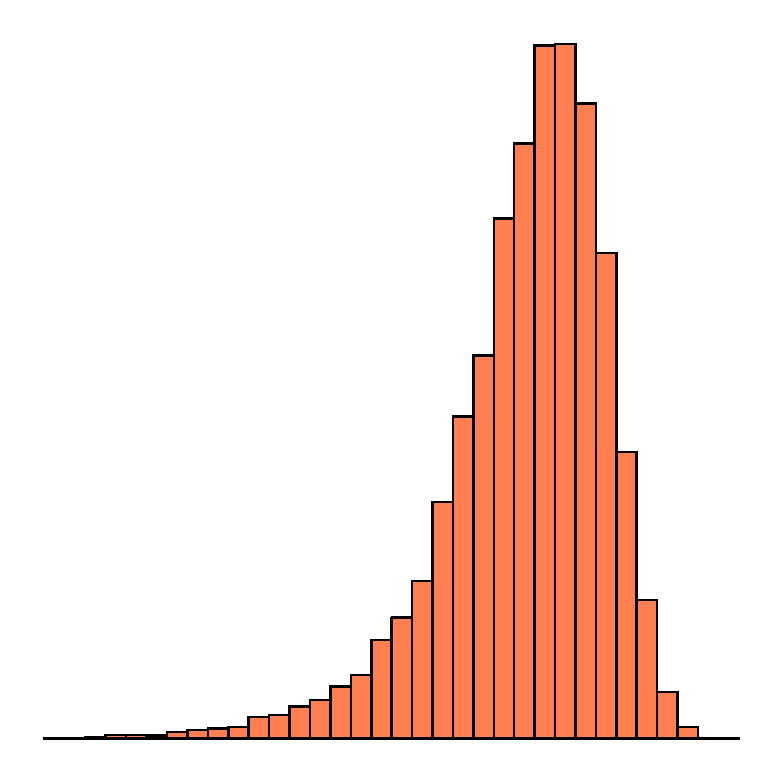
\includegraphics[scale=0.4]{img/descriptiva/histograma_asimetrico_izquierda.eps}}
\psline[linewidth=15pt,linecolor=royalblue1,arrowlength=1,arrowinset=0]{->}(5,3)(7,3)
\rput(6,3){$Y=X^2$}
\rput[l](7,3){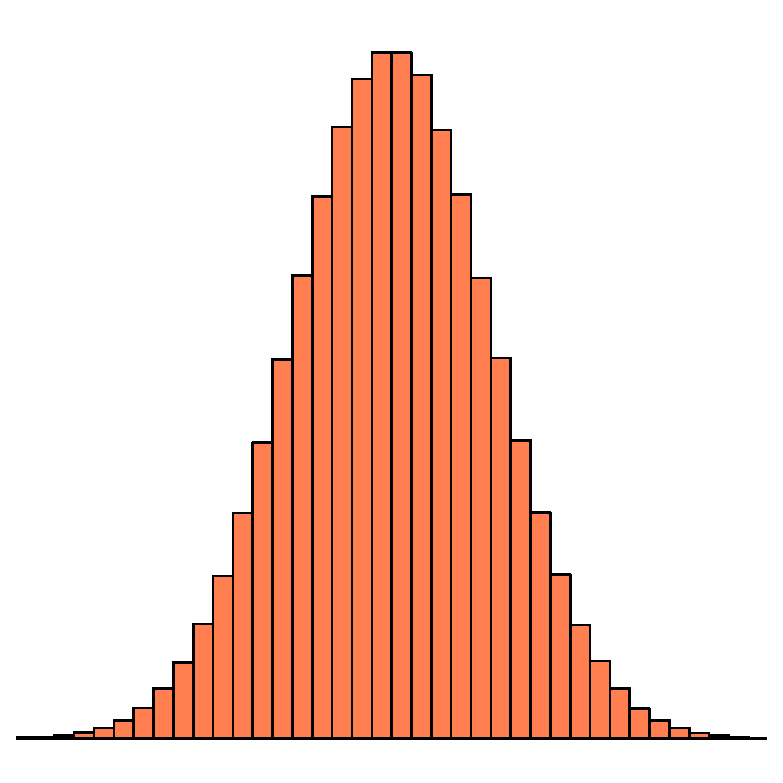
\includegraphics[scale=0.4]{img/descriptiva/histograma_simetrico.eps}}
\end{pspicture}}
\end{center}

\note{Otras transformaciones no lineales que son habituales para corregir anormalidades de la muestra son el cuadrado, que comprime la
escala para valores pequeños y la expande para valores altos, de manera que es muy útil para corregir asimetrías hacia la izquierda, tal y
como puede apreciarse en estos histogramas.
}
\end{frame}


%---------------------------------------------------------------------slide----
\begin{frame}
\frametitle{Transformaciones no lineales}
Las transformaciones $Y=\sqrt x$, $Y= \log X$ y $Y=1/X$ comprimen la escala para valores altos y la expanden para valores pequeños, de manera que son útiles para corregir asimetrías hacia la
derecha.
\begin{center}
\scalebox{1}{
\begin{pspicture}(0,0)(12,6)
\rput[l](0,3){\reflectbox{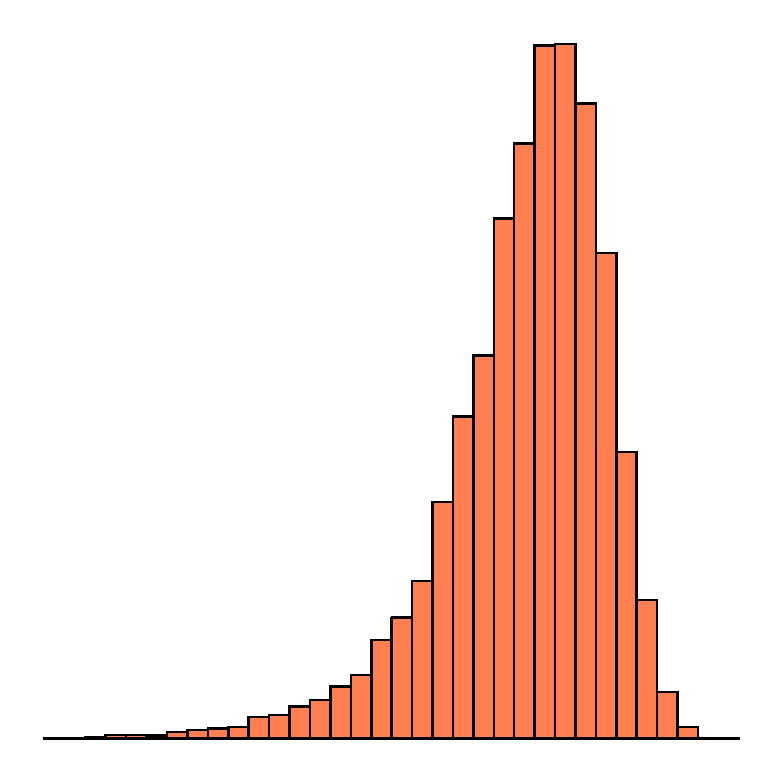
\includegraphics[scale=0.4]{img/descriptiva/histograma_asimetrico_izquierda.eps}}}
\psline[linewidth=15pt,linecolor=royalblue1,arrowlength=1,arrowinset=0]{->}(5,3)(7,3)
\rput(6,3){$Y=\sqrt{X}$}
\rput[l](7,3){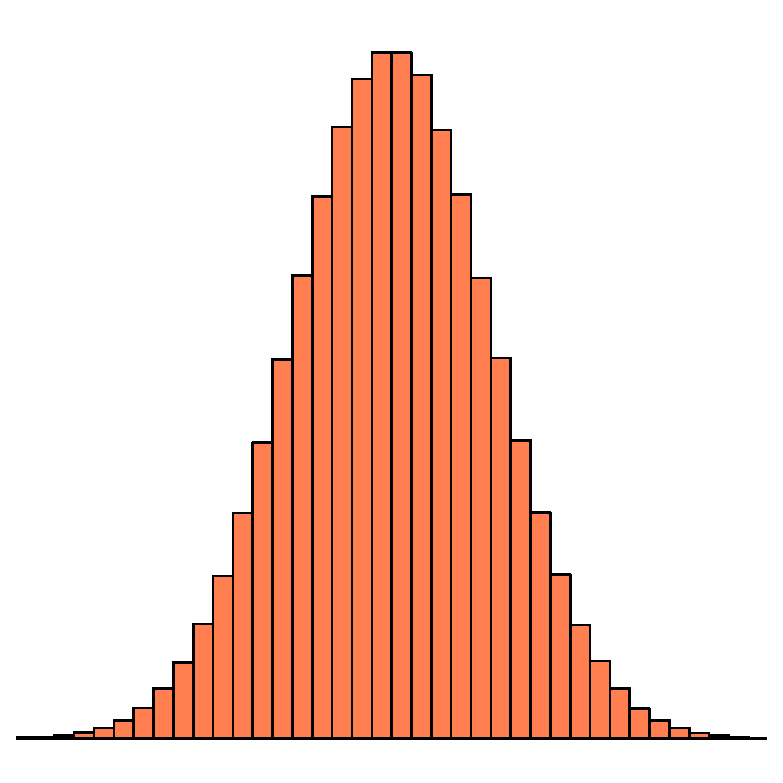
\includegraphics[scale=0.4]{img/descriptiva/histograma_simetrico.eps}}
\end{pspicture}}
\end{center}

\note{Mientras que para corregir asimetrías hacia la derecha se utilizan o bien la raíz cuadrada, la función logarítmica o la inversa, ya
que ambas comprimen la escala para valores altos y la expanden para valores pequeños.}
\end{frame}



%---------------------------------------------------------------------slide----
\begin{frame}
\frametitle{Variables clasificadoras o factores}
En ocasiones interesa describir el comportamiento de una variable, no para toda la muestra, sino para distintos grupos de individuos, como por ejemplo, estudiar las estaturas en hombres y mujeres por separado. 

En tal caso se utiliza una nueva variable, llamada \structure{\textbf{variable clasificadora}} o \structure{\textbf{factor discriminante}}, para dividir la muestra en grupos y posteriormente se realiza el estudio descriptivo de la variable principal en cada grupo.
\note{En ocasiones interesa describir el comportamiento de una variable, no para toda la muestra, sino para distintos grupos de individuos,
como por ejemplo, estudiar las estaturas en hombres y mujeres por separado.

En tal caso se utiliza una nueva variable, llamada \structure{\textbf{variable clasificadora}} o \structure{\textbf{factor discriminante}},
para dividir la muestra en grupos y posteriormente se realiza el estudio descriptivo de la variable principal en cada grupo. }
\end{frame}


%---------------------------------------------------------------------slide----
\begin{frame}
\frametitle{Variables clasificadoras}
Usando la misma muestra de estaturas, pero teniendo en cuenta el sexo, tenemos:
\begin{center}
\begin{tabular}{lll}
\hline
\multirow{2}{*}{Mujeres} &
173, 158, 174, 166, 162, 177, 165, 154, 166, 182, \\
& 169, 172, 170, 168. \\
\hline
\multirow{2}{*}{Hombres} &
179, 181, 172, 194, 185, 187, 198, 178, 188, 171,\\ 
& 175, 167, 186, 172, 176, 187. \\
\hline
\end{tabular}
\end{center}
\begin{center}
\scalebox{0.5}{%% Input file name: histograma_estatura_sexo.fig
%% FIG version: 3.2
%% Orientation: Landscape
%% Justification: Flush Left
%% Units: Inches
%% Paper size: A4
%% Magnification: 100.0
%% Resolution: 1200ppi

\begin{pspicture}(6.06cm,3.48cm)(16.82cm,13.45cm)
\psset{unit=0.8cm}
%%
%% Depth: 2147483647
%%
\newgray{mycolor0}{0.74}\definecolor{mycolor0}{gray}{0.74}
\newrgbcolor{mycolor1}{1.00 0.50 0.31}\definecolor{mycolor1}{rgb}{1.00,0.50,0.31}
\newrgbcolor{mycolor2}{0.28 0.46 1.00}\definecolor{mycolor2}{rgb}{0.28,0.46,1.00}
%%
%% Depth: 100
%%
\psset{linestyle=solid,linewidth=0.03175,linecolor=black,fillstyle=none}
\pspolygon(15.27,6.80)(15.27,8.43)(15.27,8.43)(15.27,6.80)(15.27,6.80)
\pspolygon(15.27,8.43)(15.27,10.06)(14.26,10.06)(14.26,8.43)(15.27,8.43)
\pspolygon(15.27,10.06)(15.27,11.69)(11.75,11.69)(11.75,10.06)(15.27,10.06)
\pspolygon(15.27,11.69)(15.27,13.32)(12.25,13.32)(12.25,11.69)(15.27,11.69)
\pspolygon(15.27,13.32)(15.27,14.95)(14.26,14.95)(14.26,13.32)(15.27,13.32)
\rput(15.27,15.99){\textbf{Histograma de estaturas por sexo}}
\psline(10.23,6.47)(20.31,6.47)
\psline(10.23,6.47)(10.23,6.30)
\psline(12.75,6.47)(12.75,6.30)
\psline(15.27,6.47)(15.27,6.30)
\psline(17.79,6.47)(17.79,6.30)
\psline(20.31,6.47)(20.31,6.30)
\rput(10.23,5.84){10}
\rput(12.75,5.84){5}
\rput(15.27,5.84){0}
\rput(17.79,5.84){5}
\rput(20.31,5.84){10}
\psline(10.23,6.80)(10.23,14.95)
\psline(10.23,6.80)(10.06,6.80)
\psline(10.23,8.43)(10.06,8.43)
\psline(10.23,10.06)(10.06,10.06)
\psline(10.23,11.69)(10.06,11.69)
\psline(10.23,13.32)(10.06,13.32)
\psline(10.23,14.95)(10.06,14.95)
\rput{90}(9.85,6.80){150.0}
\rput{90}(9.85,8.43){160.0}
\rput{90}(9.85,10.06){170.0}
\rput{90}(9.85,11.69){180.0}
\rput{90}(9.85,13.32){190.0}
\rput{90}(9.85,14.95){200.0}
\rput(13.18,4.86){Hombres}
\rput[r](18.17,4.86){Mujeres}
\rput{90}(8.88,10.88){Estatura}
\psline(15.27,6.47)(15.27,15.28)
\psline(10.23,6.47)(20.31,6.47)(20.31,15.28)(10.23,15.28)(10.23,6.47)
\psset{linestyle=dotted,linecolor=mycolor0}
\psline(10.23,6.47)(10.23,15.28)
\psline(11.24,6.47)(11.24,15.28)
\psline(12.25,6.47)(12.25,15.28)
\psline(13.26,6.47)(13.26,15.28)
\psline(14.26,6.47)(14.26,15.28)
\psline(15.27,6.47)(15.27,15.28)
\psline(16.28,6.47)(16.28,15.28)
\psline(17.29,6.47)(17.29,15.28)
\psline(18.29,6.47)(18.29,15.28)
\psline(19.30,6.47)(19.30,15.28)
\psset{linestyle=solid,linecolor=black,fillstyle=solid,fillcolor=mycolor1}
\pspolygon(15.27,6.80)(15.27,8.43)(15.27,8.43)(15.27,6.80)(15.27,6.80)
\pspolygon(15.27,8.43)(15.27,10.06)(14.26,10.06)(14.26,8.43)(15.27,8.43)
\pspolygon(15.27,10.06)(15.27,11.69)(11.75,11.69)(11.75,10.06)(15.27,10.06)
\pspolygon(15.27,11.69)(15.27,13.32)(12.25,13.32)(12.25,11.69)(15.27,11.69)
\pspolygon(15.27,13.32)(15.27,14.95)(14.26,14.95)(14.26,13.32)(15.27,13.32)
\psset{fillcolor=mycolor2}
\pspolygon(15.27,6.80)(15.27,8.43)(16.28,8.43)(16.28,6.80)(15.27,6.80)
\pspolygon(15.27,8.43)(15.27,10.06)(18.29,10.06)(18.29,8.43)(15.27,8.43)
\pspolygon(15.27,10.06)(15.27,11.69)(17.29,11.69)(17.29,10.06)(15.27,10.06)
\pspolygon(15.27,11.69)(15.27,13.32)(15.78,13.32)(15.78,11.69)(15.27,11.69)
\pspolygon(15.27,13.32)(15.27,14.95)(15.27,14.95)(15.27,13.32)(15.27,13.32)
\end{pspicture}
%% End
}
\quad
\scalebox{0.5}{%% Input file name: diagrama_cajas_estatura_sexo.fig
%% FIG version: 3.2
%% Orientation: Landscape
%% Justification: Flush Left
%% Units: Inches
%% Paper size: A4
%% Magnification: 100.0
%% Resolution: 1200ppi

\begin{pspicture}(6.06cm,3.48cm)(16.66cm,13.45cm)
\psset{unit=0.8cm}
%%
%% Depth: 2147483647
%%
\newrgbcolor{mycolor0}{1.00 0.50 0.31}\definecolor{mycolor0}{rgb}{1.00,0.50,0.31}
\newrgbcolor{mycolor1}{0.28 0.46 1.00}\definecolor{mycolor1}{rgb}{0.28,0.46,1.00}
%%
%% Depth: 100
%%
\psset{linestyle=solid,linewidth=0.0635,linecolor=black,fillstyle=none}
\psline(11.07,11.53)(14.81,11.53)
\psset{linestyle=dashed,linewidth=0.03175}
\psline(12.94,9.57)(12.94,10.39)
\psline(12.94,14.63)(12.94,12.83)
\psset{linestyle=solid}
\psline(12.01,9.57)(13.87,9.57)
\psline(12.01,14.63)(13.87,14.63)
\psline(11.07,10.39)(14.81,10.39)(14.81,12.83)(11.07,12.83)(11.07,10.39)
\psset{linewidth=0.0635}
\psline(15.74,9.73)(19.47,9.73)
\psset{linestyle=dashed,linewidth=0.03175}
\psline(17.60,7.45)(17.60,9.25)
\psline(17.60,12.02)(17.60,10.55)
\psset{linestyle=solid}
\psline(16.67,7.45)(18.54,7.45)
\psline(16.67,12.02)(18.54,12.02)
\psline(15.74,9.25)(19.47,9.25)(19.47,10.55)(15.74,10.55)(15.74,9.25)
\psline(12.94,6.47)(17.60,6.47)
\psline(12.94,6.47)(12.94,6.26)
\psline(17.60,6.47)(17.60,6.26)
\rput(12.94,5.71){hombre}
\rput(17.60,5.71){mujer}
\psline(10.23,6.80)(10.23,14.95)
\psline(10.23,6.80)(10.02,6.80)
\psline(10.23,8.43)(10.02,8.43)
\psline(10.23,10.06)(10.02,10.06)
\psline(10.23,11.69)(10.02,11.69)
\psline(10.23,13.32)(10.02,13.32)
\psline(10.23,14.95)(10.02,14.95)
\rput{90}(9.73,6.80){150}
\rput{90}(9.73,8.43){160}
\rput{90}(9.73,10.06){170}
\rput{90}(9.73,11.69){180}
\rput{90}(9.73,13.32){190}
\rput{90}(9.73,14.95){200}
\rput(15.27,15.99){\textbf{Diagrama de caja y bigotes de estaturas por sexo}}
\rput(15.27,4.86){Sexo}
\rput{90}(8.88,10.88){Estatura}
\psline(10.23,6.47)(20.31,6.47)(20.31,15.28)(10.23,15.28)(10.23,6.47)
\end{pspicture}
%% End
}
\end{center}

\note{Si en el ejemplo de las estaturas hubiesemos tomado el sexo como factor, la muestra quedaría dividida en dos grupos, los hombres y
las mujeres, y podríamos hacer un estudio descriptivo por separado de cada grupo para luego compararlos.}
\end{frame}
\end{document}
